\documentclass[a4paper, 8pt]{extarticle}
\setcounter{page}{0}


\usepackage[pdfencoding=auto, psdextra]{hyperref}

\usepackage[landscape]{geometry}
\geometry{
     %total={210mm,297mm},
     left=2mm,
     right=2mm,
     top=15mm,
     bottom=0mm,
 }
\usepackage[utf8]{inputenc}
\usepackage[normalem]{ulem}

\usepackage{amssymb}
\usepackage{amsmath}
\usepackage{amsfonts}

\usepackage{mathtools}
\usepackage[ngerman]{babel}

\usepackage{multicol} %multiple columns

%get rid of spacing between lists
% \usepackage{enumitem} 
    % \setlist{nolistsep}

%imagepackage
\usepackage{float}
\usepackage{graphicx} 
    \graphicspath{ {./images/} }

\usepackage{parskip} %Einzug aus, Absatzabstand ein
    \tolerance=2000 %Toleranz für Wortzwischenräume
    \setlength{\emergencystretch}{20pt} %Zusätzliche Zeilendehnbarkeit in Notfällen
    \setlength\parindent{0pt}
    \setlength{\columnseprule}{1px} %thickness of column seperator

%New Titles
\usepackage{tcolorbox}
    \definecolor{seccol}{RGB}{7, 61, 50}
    \definecolor{subseccol}{RGB}{29, 120, 116}
    \definecolor{subsubseccol}{RGB}{103, 146, 137}

\usepackage[explicit]{titlesec}

\titleformat{\section}
  {\normalfont\bfseries}
  {}
  {0em}
  {\pgfsetfillopacity{1}
    \colorbox{seccol}{
        \parbox{\dimexpr\linewidth-4.5\fboxsep\relax}{
            \textcolor{white}{\thesection\quad#1}}}
    \pgfsetfillopacity{1}}
  
\titleformat{\subsection}
  {\normalfont\bfseries}
  {}
  {0em}
  {\pgfsetfillopacity{1}
    \colorbox{subseccol}{
        \parbox{\dimexpr\linewidth-4.5\fboxsep\relax}{
            \textcolor{white}{\thesubsection\quad#1:}}}
    \pgfsetfillopacity{1}}

\titleformat{\subsubsection}
  {\normalfont\bfseries}
  {}
  {0em}
  {\pgfsetfillopacity{1}
    \colorbox{subsubseccol}{
        \parbox{\dimexpr\linewidth-4.5\fboxsep\relax}
            {\textcolor{white}{\thesubsubsection\quad#1:}}}
    \pgfsetfillopacity{1}}
    
\titlespacing{\section}{0pt}{\parskip}{-0.75\parskip}    
\titlespacing{\subsection}{0pt}{\parskip}{-0.75\parskip}
\titlespacing{\subsubsection}{0pt}{\parskip}{-0.75\parskip}

%custom header with title & authors
\usepackage{fancyhdr} 
    \pagestyle{fancy}
    \fancyhf{}
    \rhead{Joshua Näf and Franz Büelmä \textit{naefjo@ethz.ch, franzbu@ethz.ch}}
    \chead{\textbf{\thepage}}
    \lhead{\textbf{Control Systems II Spring 20 Prof. Dr. L. Guzzella}}
    \setlength{\headsep}{1mm}


%colourful boxes for math mode
% Syntax: \colorboxed[<color model>]{<color specification>}{<math formula>}
\usepackage{xcolor}
\newcommand*{\colorboxed}{}
\def\colorboxed#1#{%
  \colorboxedAux{#1}%
}
\newcommand*{\colorboxedAux}[3]{%
  % #1: optional argument for color model
  % #2: color specification
  % #3: formula
  \begingroup
    \colorlet{cb@saved}{.}%
    \color#1{#2}%
    \boxed{%
      \color{cb@saved}%
      #3%
    }%
  \endgroup
}    


%TODO command    
\newcommand{\TODO}[1]{\large\textcolor{red}{\textbf{TODO: #1\\}}\normalsize}

%New commands
\newcommand{\jw}{j\omega}
    
    
\title{Control Systems II}
\author{Joshua Näf \& Franz Büelmä}
\date{}

\begin{document}

\maketitle
\begin{center}
    \parbox{0.5\linewidth}{\begin{center}
        This summary has been written based on the Lecture 151-0590-00L Regelungstechnik II by Prof. Dr. Guzzella (FS20) and the weekly theory sheets provided by C. Küttel. There is no guarantee for completeness and/or correctness regarding the content of this summary. Use it at your own discretion.
        
        Source Code: \url{https://github.com/franzbu-png/control-systems-2}
    \end{center}}
\end{center}
\newpage

\begin{center}
    \begin{multicols*}{3}
        \tableofcontents
    \end{multicols*}
\end{center}

\begin{multicols*}{2}
\section{MATLAB Cheat Sheet}
        \begin{center}
    {\def\arraystretch{1.4}
    \begin{tabular}{p{5cm}|p{8.5cm}}
        \textbf{Command}    &   \textbf{Description}\\
        \hline
        \texttt{bode(SYS)}  &  Draws the Bode plot of the dynamic system SYS.\\
        
        \texttt{[MAG,PHASE] = bode(SYS,W) [MAG,PHASE,W] = bode(SYS)} & Return the response magnitudes and phases in degrees (along with the frequency vector W if unspecified).  No plot is drawn on the screen. \\
        
        \texttt{W = logspace(-2,3,1e3)} & $10^{-2} < w < 10^3$ mit 1000 log-Werten\\
        
        \texttt{nyquist(SYS)}  &  Draws the Nyquist plot of the dynamic system SYS. \\
        
        \texttt{[RE,IM] = nyquist(SYS,W) [RE,IM,W] = nyquist(SYS)} & Return the real parts RE and imaginary parts IM of the frequency response (along with the frequency vector W if unspecified).\\
        
        \texttt{sys = ss(A,B,C,D)}  & Creates an object SYS representing the continuous-time state-space model \\
        
        \texttt{(E =) [V,D] = eig(A)}  &  Produces a diag matrix D of eigenvalues and a matrix V whose columns are eigenvectors so that A*V = V*D. (Column vector E containing the Eigval of a matrix A.)\\
        
        \texttt{co = ctrb(A,B) (= ctrb(SYS))}  & Returns the controllability matrix $[B AB A^2B ...]$.  \\
        
        \texttt{ob = obsv(A,C) (= obsv(SYS))}  & Returns the observability matrix $[C; CA; CA^2 ...]$ \\
        
        \texttt{s = tf('s')}  & Specifies the transfer function H(s) = s (Laplace variable). \\
        
        \texttt{SYS = tf(NUM,DEN, \textcolor{blue}{Ts}, 'InputDelay', T)} & Creates a continuous-time transfer function SYS with numerator NUM and denominator DEN and optinal time delay $T$. (For discrete-time models add a sample time $T_s$)\\
        
        \texttt{P = tf(sys)}  & Converts any dynamic system SYS to the transfer function representation. \\
        
        \texttt{MSYS = minreal(SYS)}  &  Produces, for a given LTI model SYS, an equivalent model MSYS where all cancelling pole/zero pairs or non minimal state dynamics are eliminated.  For state-space models, minreal produces a minimal realization MSYS of SYS where all uncontrollable or unobservable modes have been removed.\\
        
        \texttt{X = fminsearch(FUN,X0)}  &  Starts at X0 and attempts to find a local minimizer X of the function FUN.  FUN is a function handle.  FUN accepts input X and returns a scalar function value F evaluated at X. X0 can be a scalar, vector or matrix.\\
        
        \texttt{P = pole(SYS))}  & Returns poles P of the dynamic system SYS as a column vector. For state-space models, the poles are the eigenvalues of the A matrix. (Bei MIMO System die Pole der SISO-Elemente) \\
        
        \texttt{[Z,G] = zero(SYS)} & Computes the zeros Z and gain G of the single-input, single-output dynamic system SYS.\\
        
        \texttt{Z = tzero(SYS,TOL)}  &  Computes invariant zeros of the dynamic system SYS. For state-space models with matrices A,B,C,D,E (= I), the invariant zeros are the complex values s for which the rank of the matrix $\begin{bmatrix} A -sE & B\\ C & D\end{bmatrix}$ drops below its normal value. For minimal realizations, this coincides with the transmission zeros of SYS (values of s for which its transfer function drops rank).\\ 
        
        \texttt{Ydb = mag2db(Y)} & Converts magnitude data Y into dB values. (db2mag analog)\\
 
        \texttt{[NUM,DEN] = tfdata(SYS)} & Returns the num. and denom. of the transfer function SYS.
        
        
    \end{tabular}

    \begin{tabular}{p{5cm}|p{8.5cm}}
        \textbf{Command}    &   \textbf{Description}\\
        \hline
        \texttt{[Z,P,K] = tf2zp(NUM,DEN)} & Finds the zeros, poles, and gains from a transferfunction in the form of $\displaystyle H(s) = K\cdot\frac{(s-z1)(s-z2)\dots(s-zn)}{(s-p1)(s-p2)\dots(s-pn)}$\\
        
        \texttt{[Z,P,K] = zpkdata(SYS)} & Returns the zeros, poles, and gain for each I/O channel of the dynamic system SYS.\\
        
        \texttt{K = dcgain(SYS)} & Computes the steady-state (D.C. or low frequency) gain of the dynamic system SYS \big($P(j\cdot0)$\big)\\
        
        \texttt{eye(M)/ eye(M,N)/ eye(size(A))}  &  M-by-M/M-by-N/siz(A) matrix with 1's on the diagonal and zeros elsewhere. \\
        
        \texttt{zeros(M)/ zeros(M,N)/ zeros(size(A))}  &  M-by-M/M-by-N/size(A) matrix of zeros.\\
        
        \texttt{rga = P.*inv(P')}  &  MATLAB code to compute the RGA matrix of P\\
        
        \texttt{bodemag(SYS)}  &  Plots the magnitude of the frequency response of the linear system SYS (useful for RGA/\textbf{Bode plot without the phase diagram}). \\
        
        \texttt{sigma(SYS)}  &  Produces a singular value (SV) plot of the frequency response of the dynamic system SYS.\\
        
        \texttt{[U,S,V] = svd(X)}  &  Produces a diagonal matrix S, of the same dimension as X and with nonnegative diagonal elements in decreasing order, and unitary matrices U and V so that $X = U\cdot S\cdot V^\top$.\\
        
        \texttt{FRESP = evalfr(SYS,X)}  & Evaluates the transfer function of the continuous- or discrete-time linear model SYS at the complex number S=X or Z=X. \textbf{X = j$\cdot$omega} (Eval System, then plug it into svd)\\
        
        \texttt{SimOut = sim('MODEL', PARAMETERS)}  & Simulates your Simulink model, where 'PARAMETERS' represents a list of parameter name-value pairs. \\
        
        \texttt{L = series(C,P)}  & Connects the input/ouput models $C$ and $P$ in series. \\
        
        \texttt{M = feedback(M1,M2)}  & $(M1,M2) = (1,L) \Rightarrow S(s)$ and  $(M1,M2) = (L,1) \Rightarrow T(s)$. Computes a closed-loop model M (assumes negative feedback: for positive add ",+1")\\
        
        $\mathtt{\mu_{\textnormal{min}} = min( abs(bode(1 + L)))}$ &  Computes the minimum return difference of a given open loop gain $L$\\
        
        \texttt{[Gm,Pm,Wcg,Wcp] = margin(SYS)}  & Computes the gain margin Gm, the phase margin Pm, and the associated frequencies Wcg and Wcp, for the SISO open-loop model SYS. The gain margin Gm is defined as 1/G where G is the gain at the -180 phase crossing. The phase margin Pm is in degrees. $\mathbf{k_p^* = Gm, \, T^* = \frac{2\pi}{Wcg}}$\\
        
        \texttt{margin(SYS)} & Creates a Bode plot of the open loop and marks the gain and phase margins in the plot. \\
        
        \texttt{B = squeeze(A)}  &  Returns an array B with the same elements as A but with all the singleton dimensions removed.\\
        
        \texttt{SYSD = c2d(SYSC,TS,METHOD)}  &  Computes a discrete-time model SYSD with sample time TS that approximates the continuous-time model SYSC (method = zoh, foh, impulse, tustin,...)\\
        
        \texttt{SYSC = d2c(SYSD,METHOD)} & Computes a continuous-time model SYSC that approximates the discrete-time model SYSD. (method = as above)\\
        
        \texttt{[K,S,CLP] = lqr(SYS,Q,R) = lqr(A,B,Q,R)} & Calculates the optimal gain matrix K for the continuous or discrete state-space model SYS. lqr also returns the solution S of the associated algebraic Riccati equation and the closed-loop poles \texttt{CLP = eig(A-B*K)}.\\
        
        \texttt{Ki\_lqri = -K\_tilde(:,n+1:end)} & Extraction of $K_I$ from $\Tilde{K}$
    \end{tabular}
}
\end{center}


\newpage

        
\end{multicols*}
\begin{multicols*}{3}

\section{Recap}
        \subsection{Umrechnung zwischen Dezimal und Dezibel}
    \begin{equation*}
        |\Sigma(s)|_{dB} = 20 \cdot \textrm{log}_{10}|\Sigma(s)| =             20\cdot\frac{\textrm{ln}(|\Sigma(s)|)}{\textrm{ln}(10)}
    \end{equation*}
    \begin{equation*}
        |\Sigma(s)| = 10^{\frac{|\Sigma(s)|_{dB}}{20}}
    \end{equation*}
    \begin{center}
    {\renewcommand{\arraystretch}{1.4}
        \begin{tabular}{c|c}
        Dezimalskala    &   Dezibelskala [dB]\\
        \hline
        100 &   40  \\
        10  &   20  \\
        5   &   13.97..\\
        3.16.. & 10\\
        2   &   6.02..\\
        1   &   0   \\
        $\frac{1}{\sqrt{2}}$  &   -3.0103\\
        0.316.. & -10\\
        0.1 &   -20 \\
        0.01    &   -40\\
        0       &   $-\infty$
        \end{tabular}}
    \end{center}
    \begin{equation*}
        |\Sigma(j\omega)|_{dB} = |\Sigma_1(j\omega)|_{dB}+|\Sigma_2(j\omega)|_{dB}
    \end{equation*}
    \begin{equation*}
        \angle\Sigma= \angle\Sigma_{1}+ \angle\Sigma_{2}
    \end{equation*}
    \begin{equation*}
        \angle\Sigma(j\omega)=
        \begin{cases}
            \arctan(\frac{x}{y}) & x > 0\\
            \arctan(\frac{x}{y})+\pi & x<0
        \end{cases}
    \end{equation*}
    
\subsection{Übertragungsfunktionen}
    Matrix mit den herkömmlichen Übertragungsfunktionen.
    \begin{equation*}
        \begin{bmatrix}
            U(s)\\Y(s)\\E(s)
        \end{bmatrix}
        =
        \begin{bmatrix}
            S(s)    &   -S(s)\cdot C(s) &   S(s)\cdot C(s)\\
            S(s)\cdot P(s)  &   S(s)    &   T(s)\\
            -S(s)\cdot P(s) &   -S(s)   &   S(s)
        \end{bmatrix}
        \cdot
        \begin{bmatrix}
            W(s)\\D(s)\\R(s)
        \end{bmatrix}
    \end{equation*}
    
\subsection{Nyquist Theorem/Nominelles Stabilitätskriterium von Nyquist}
    Bestimmung der Stabilität von $T(s)$ durch $L(s)$ (ohne Modellunsicherheit).
            
    Der geschlossene Regelkreis mit Übertragungsfunktion $T(s)$ ist asymptotisch stabil, falls für $L(s)$ gilt:
        \begin{equation*}
            n_c\overset{!}{=}\frac{n_0}{2}+n_+
        \end{equation*}
        \begin{tabular}{l l}
            $n_c$:  & Anzahl Umrundungen um den kritischen Punkt (-1,0)  \\
                    & Positiv falls Umrundung gegen Uhrzeigersinn.\\
            $n_0$:  & Anzahl Pole von $L(s)$ mit Realteil = 0\\
            $n_+$:  & Anzahl Pole von $L(s)$ mit Realteil $>$ 0
        \end{tabular}
  
 \subsection{Beschränkung der Durchtrittsfrequenz}
    \begin{equation*}
        \boxed{\omega_c = 
        \begin{cases}
        \omega_c > \textrm{max}\{10\cdot\omega_d, 2\cdot\omega_{\pi^+}\}\\
        \omega_c < \textrm{min}\{\frac{1}{10}\cdot\omega_n, \frac{1}{10}\cdot \omega_2, \frac{1}{2}\cdot \omega_\tau, \frac{1}{2}\cdot \omega_{\zeta^+}\}
        \end{cases}
        }
    \end{equation*} 
    
\subsection{PID - Recap}
    Der PID-Regler hat folgende Form:
    \begin{equation*}
        C_{\textnormal{PID}}(s) = k_p\cdot\left(1 + \frac{1}{T_i\cdot s} + T_d\cdot s\right) = k_p\left(\frac{T_d\cdot T_i\cdot s^2 + T_i\cdot s + 1}{T_i\cdot s}\right)
    \end{equation*}
    
    \subsubsection{Ziegler-Nichols}
    \begin{equation*}
        P(s) \approx \frac{k}{\tau\cdot s + 1}\cdot e^{-T\cdot s}, \quad \frac{T}{T+\tau} < 0.3
    \end{equation*}
        \begin{equation*}
            \boxed{|k_p^* \cdot P(j\omega^*)| \overset{!}{=} 1} \hspace{3mm}
            \boxed{\angle k_p^* \cdot P(j\omega^*)\overset{!}{=}-\pi} \hspace{3mm}
            \boxed{T^* =\frac{2\pi}{\omega^*}}
        \end{equation*}
        \begin{center}
        {\renewcommand{\arraystretch}{1.2}
            \begin{tabular}{l r r r}
            Regler & $k_p$ & $T_i$ & $T_d$ \\
                 \hline
                P & $0.5\cdot k_p^*$ & $\infty \cdot T^*$ & $0 \cdot T^*$ \\
                PI & $0.45\cdot k_p^*$ & $0.85\cdot T^*$ & $0 \cdot T^*$\\
                PD & $0.55 \cdot k_p^* $& $\infty \cdot T^*$ &  $0.15\cdot T^*$\\
                PID & $0.6\cdot k_p^*$ & $0.5 \cdot T^*$ & $0.125 \cdot T^*$\\
            \end{tabular}}
        \end{center}

\subsection{Inverse einer 2x2-Matrix}
    \begin{equation*}
        A = \begin{bmatrix} a & b \\ c & d \end{bmatrix}\quad
        A^{-1} = \frac{1}{a\cdot d - c\cdot b}\begin{bmatrix} d & -b \\ -c & a \end{bmatrix}\quad
    \end{equation*}
\subsection{Nützliche Ableitungen}
    \begin{align*}
        arctan(a \cdot x) &\xrightarrow{\frac{\partial}{\partial x}} \frac{a}{1+(ax)^2}\\ 
    \end{align*}
        
\vfill\null\newpage        
\section{PID}
    
\subsection{PID - Tuning}
    \subsubsection{\r{A}ström-Hägglund Verfahren}
        Spezifikation des Reglers anhand von $\{k_p^*, T^*, |P(0)|\}$. Zusätzliche Auswahl zwischen agressiven/robusten Regler ($\mu_{\textnormal{min}} \approx 0.5$/ $\mu_{\textnormal{min}} \approx 0.7$)
        % Man spezifiziert seinen Regler anhand $k_p^*, T^*, |P(0)|$. Zusätzlich kann man zwischen einem aggressiven Regler ($\mu_{\textnormal{min}} \approx 0.5$) oder einem robusten Regler ($\mu_{\textnormal{min}} \approx 0.7$) auswählen.
        \[\{k_p^*,\ T^*,\ |P(0)|,\ \mu_{\textnormal{min}}\} \rightarrow \{k_p,\ T_i,\ T_d\}\]
            \begin{center}
            \begin{tabular}{c|c c c|c c c}
                & & $\mu_{\textnormal{min}} = 0.7$ & & &  $\mu_{\textnormal{min}} = 0.5$ & \\ 
                x & $\alpha_{0,x}$ & $\alpha_{1,x}$ & $\alpha_{2,x}$ & $\alpha_{0,x}$ & $\alpha_{1,x}$ & $\alpha_{2,x}$ \\ \hline
                $k_p/k_p^*$  & 0.053 & 2.90 & -2.60 & 0.13 & 1.90 & -1.30 \\
                $Ti/T^*$ & 0.90 & -4.40 & 2.70 & 0.90 & -4.40 & 2.70\\ 
                $a$  &  1.10  &  -0.0061  &  1.8  &   0.48  &  0.40  &  -0.17\\
            \end{tabular}
            \r{A}ström-Hägglund Koeffizienten für PI-Regler

        
            \begin{tabular}{c|c c c|c c c}
                & & $\mu_{\textnormal{min}} = 0.7$ & & &  $\mu_{\textnormal{min}} = 0.5$ & \\ 
                x &
                $\alpha_{0,x}$ & $\alpha_{1,x}$ & $\alpha_{2,x}$ & $\alpha_{0,x}$ & $\alpha_{1,x}$ & $\alpha_{2,x}$ \\ \hline
                $k_p/k_p^*$  & 0.33 & -0.31 & -1.00 & 0.72 & -1.60 & 1.20 \\
                $Ti/T^*$ & 0.76 & -1.60 & -0.36 & 0.59 & -1.30 & 0.38 \\
                $T_d/T^*$ & 0.17 & -0.46 & -2.10 & 0.15 & -1.40 & 0.56\\
                $a$  &  0.58  &  -1.3000  &  3.5  &   0.25  &  0.56  &  -1.20\\
            \end{tabular}    
            \r{A}ström-Hägglund Koeffizienten für PID-Regler 
            
            \end{center}
            
            mit diesen Parametern können wir $\square \in \{a, k_p,\, T_i,\, T_d\}$ bestimmen.
            \[ \square = \square^* \cdot \alpha_{0,x} \cdot e^{\alpha_{1,x} \cdot \kappa + \alpha_{2,x} \cdot \kappa^2}
            \ \textnormal{mit} \ \kappa = \frac{1}{|P(0)| \cdot k_p^*} \]
            \textbf{Note:}
            \begin{itemize}
                \item $T^* = T_i^*,\  T_d^*$ oftmals gibt \r{A}ström-Hägglund Verfahren bessere Resultate als Ziegler-Nichols. Dies ist jedoch nicht immer der Fall. 
                \item Beim set point weight $a$ wählt man für $a^* = 1$ 
                \item Das Design ist nicht garantiert gut oder stabil, dementsprechend soll ein a postepriori Test der closed-loop Stabilität, Frequenz Antwort der Kreisverstärkung, Simulation der Störrungsunterdrückung des closed-loop System durchgeführt werden.
            \end{itemize}
            
    \subsubsection{Direktspezifikationen} 
        Ziel der Direktspezifikation ist die PID- parameter so zu wählen, dass die Kreisverstärkung $L(s)$ die gewünschte \textbf{Übergangsfrequenz $\omega_c$}, \textbf{Phasenereserve} $\varphi$ und \textbf{Steigung} $\psi$ erzielt. Zusätzlich brauchen wir noch 
        \begin{align*}
        r_P &= |P(j\omega_c)|   &   \varphi_P &= \angle P(j\omega_c)\\
        r'_P &= \frac{\partial r_P(\omega)}{\partial\omega}\Bigg|_{\omega=\omega_c} & \varphi'_P &= \frac{\partial \varphi_P(\omega)}{\partial\omega}\Bigg |_{\omega=\omega_c}
        \end{align*}
        Mit diesen Werten können wir nun die PID-Parameter bestimmen:
        \[k_P = - \frac{1}{r_P}\cos(\varphi-\varphi_P)\]
        \begin{multline*}
        T_d =\frac{1}{2}\cdot\Bigg(\tan(\psi-\varphi_P)\Bigg(\frac{r'_P}{r_P}-\varphi'_P\tan(\varphi-\varphi_P)\Bigg)\\ + \tan(\varphi-\varphi_P) \Bigg(\frac{1}{\omega_c}-\frac{r'_P}{r_P}\Bigg)- \varphi'_P\Bigg)
        \end{multline*}
        \[T_i = (T_d\cdot \omega_c^2 - \tan(\varphi-\varphi_P)\cdot \omega_c)^{-1}\]
        \textbf{Note:}
        
        Die Stabilität ist mit diesem Verfahren nicht garantiert. Phase muss in der Formel in Radiant angegeben werden. 
\subsection{Prädikative PI Regler}
    für Regelstrecken mit wesentlicher Totzeit, das heisst falls 
    \[\frac{T}{T+\tau}>0.3\]
    kann man nicht einfach einen PID-Regler auslegen. Stattdessen legt man einen Controller aus der mit der Totzeit umgehen kann. 

    
    \subsubsection{Prädikative PI Regler für einfache Regelstrecken}
        Annahme: Regelstrecke erster Ordnung 
        \[P(s)\approx \frac{k}{\tau s + 1}\cdot e^{-Ts}\]
        man wählt die gewünschte \textbf{Sensitivität} 
        \[S(s) = 1- \frac{1}{s\cdot\sigma\cdot \tau + 1 \cdot e^{-Ts}} = 1 - T(s) \]
        mit $\sigma = $ Tuning-Parameter
        Der Kontroller der die gewünschte Kreisverstärkung erfüllt hat folgende Form 
        \[C(s) =\frac{1-S(s)}{S(s)\cdot P(s)}= \frac{\tau\cdot s+1}{k\cdot(\sigma\cdot\tau\cdot s+ 1-e^{-Ts})}\]
        Somit lautet die Eingangsgrösse: 
        \[U(s)=\underbrace{\frac{1}{\sigma k}\Bigg(1+\frac{1}{\tau\cdot s}\Bigg)E(s)}_{\textnormal{PI-Regler}} - \underbrace{\frac{1}{\sigma\tau s}(1-e^-{Ts})\cdot U(s)}_{\textnormal{Prädikitve Korrektur}}\] 
        \textbf{Note:} Falls T = 0 wird die prädikative Korrektur 0 und der resultierende Eingang wird zu einem einfachen PI - Regler.
    
    \subsubsection{Smith Predictor}
        Annahme: System hat einen rationalen Teil und eine Totzeit
        
        \[P(s) = P_r(S)\cdot e^{-Ts}\]
        \begin{figure}[H]
            \centering
            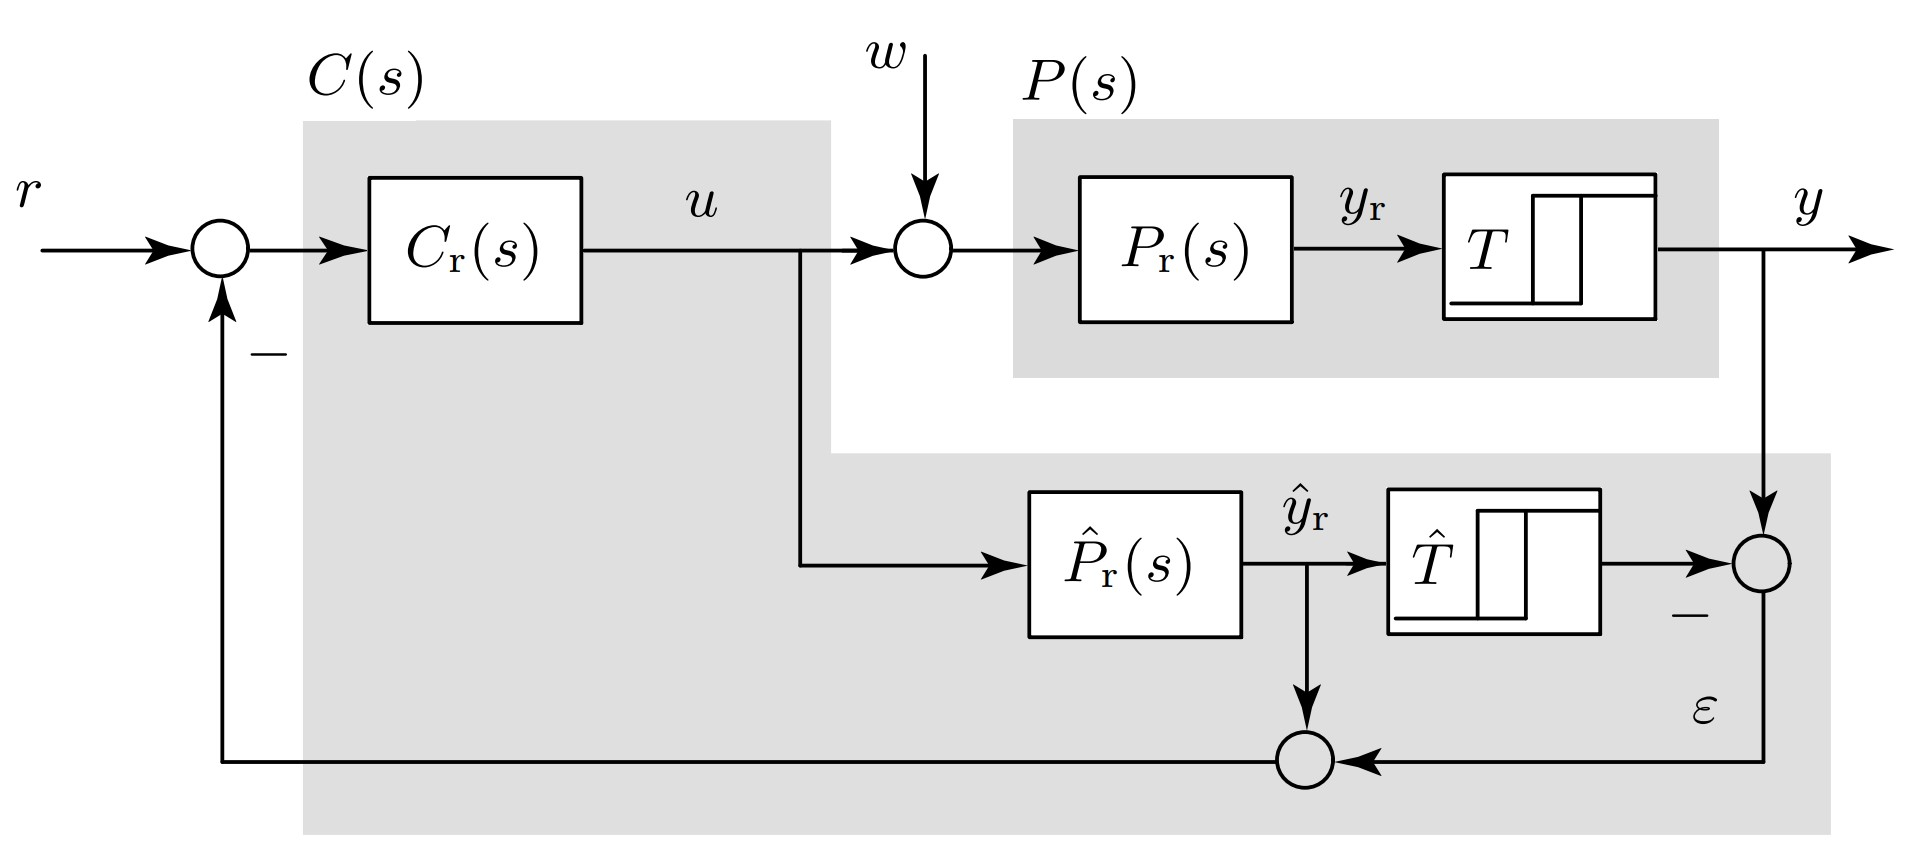
\includegraphics[width = 0.6\linewidth]{02/Smithpredictor.jpg}
            \caption{Regelstruktur eines Smith Predictors}
        \end{figure}
        \begin{figure}[H]
            \centering
            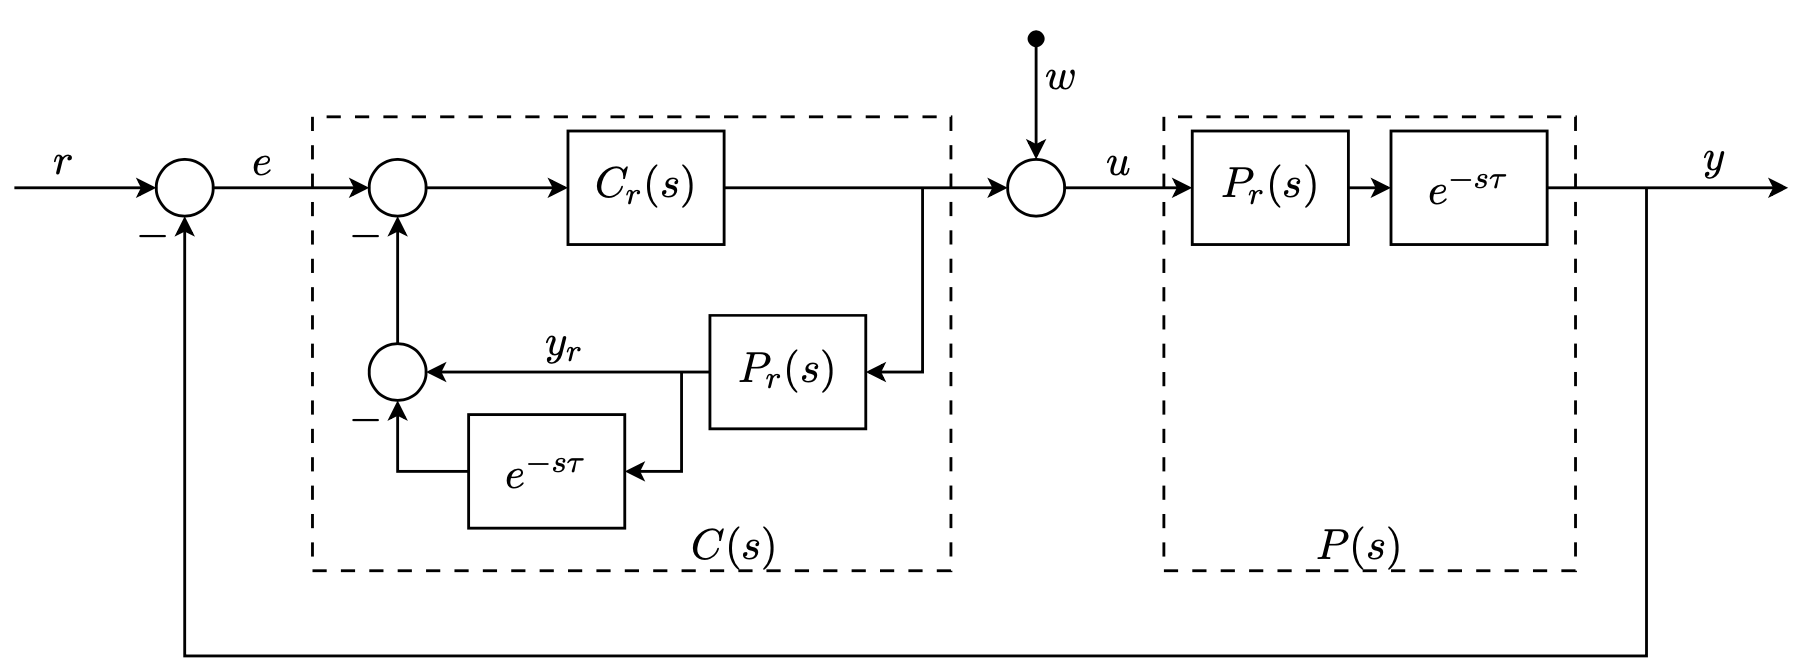
\includegraphics[width = 0.8\linewidth]{02/smithpred_alt.png}
            \caption{Alternative Darstellung des Smith Predictors}
        \end{figure}
        
        wenn es keine Modellfehler gibt ($P_r(s) = \hat P_r(s),\ T = \hat T$) und keine Störung ($\omega = 0$)($\Rightarrow \epsilon = 0$), resultiert folgende komplementäre Sensitivität:
        \begin{align*}
            L_{\textnormal{pred}} &= \underbrace{\frac{C_r(s)}{1 + C_r(s)\cdot\hat{P}_r(s)\cdot\big(1 - e^{-s\hat{T}}\big)}}_{C(s)}\cdot P_r(s)\cdot e^{-sT}\\
            \frac{Y(s)}{R(s)} &= e^{-Ts}\cdot\frac{P_r(s)C_r(S)}{1+P_r(S)C_r(s)} = e^{-Ts}\cdot T_r(S)
        \end{align*}
        Auflösen der obigen Gleichung nach $C(s)$ liefert
        \begin{equation*}
            C_r(s) = \frac{T_{\textnormal{ref}}(s)}{P_r(s)\cdot(1-T_{\textnormal{ref}}(s))}
        \end{equation*}
        wobei $T_\textnormal{ref}(s)$ die gewünschte TF von $r\rightarrow y$ ist.
        
        \textbf{Note:} 
        \begin{itemize}
            \item Falls Modellfehler und Störungen vorhanden sind wird die Gleichung für die komplementäre Sensitivität wesentlich komplizierter!
            
            \item Nicht minimalphasige NST von $P(s)$ werden zu instabilen Polen 
        \end{itemize}
        
        Schätzungsfehler von der Totzeit $T$ kann grosse Auswirkungen auf das Systemverhalten haben. Bei einem Schätzfehler von $\pm 20\%$ kann immer noch eine schnelle und robuste Systemantwort ohne übermässige Abweichungen vom Referenzsystem erzielt werden.
        \begin{figure}[H]
            \centering
            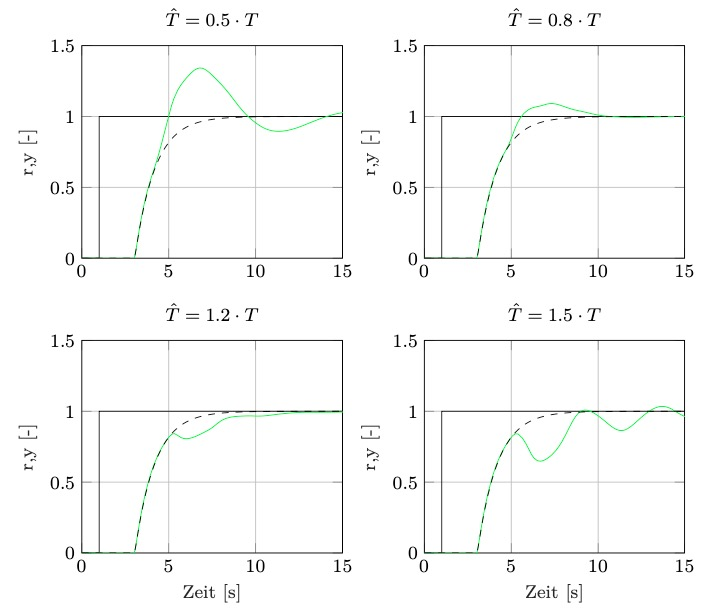
\includegraphics[width = 0.7\linewidth]{images/02/est_error_hat_T.jpg}
            \caption{Auswirkung Schätzungsfehler von $\hat{T}$ auf die Sprungantwort}
        \end{figure}
        


\vfill\null\newpage        
\section{Spezifikation der Sensitivität}
    \subsection{Multiplikative Unsicherheit von \textit{T(s)}}
    Modellunsicherheit $W_2(s)$ ist multiplikativ für die komplementäre Sensitivität eingeführt. Dies führt zum \textit{robusten Nyquist Theorem:}
    \begin{equation*}
        |T(\jw)\cdot W_2(\jw)| < 1 \Rightarrow |L(\jw)\cdot W_2(\jw)| < |1+L(\jw)|
    \end{equation*}
    Im Bode-Plot kann man das relativ einfach überprüfen, indem man schaut ob folgende Ungleichung erfüllt ist.
    \begin{equation*}
        |T(\jw)| <  |W_2^{-1}(\jw)|
    \end{equation*}
    
    Man kann das wie folgt geometrisch interpretiern:
    \begin{figure}[H]
        \centering
        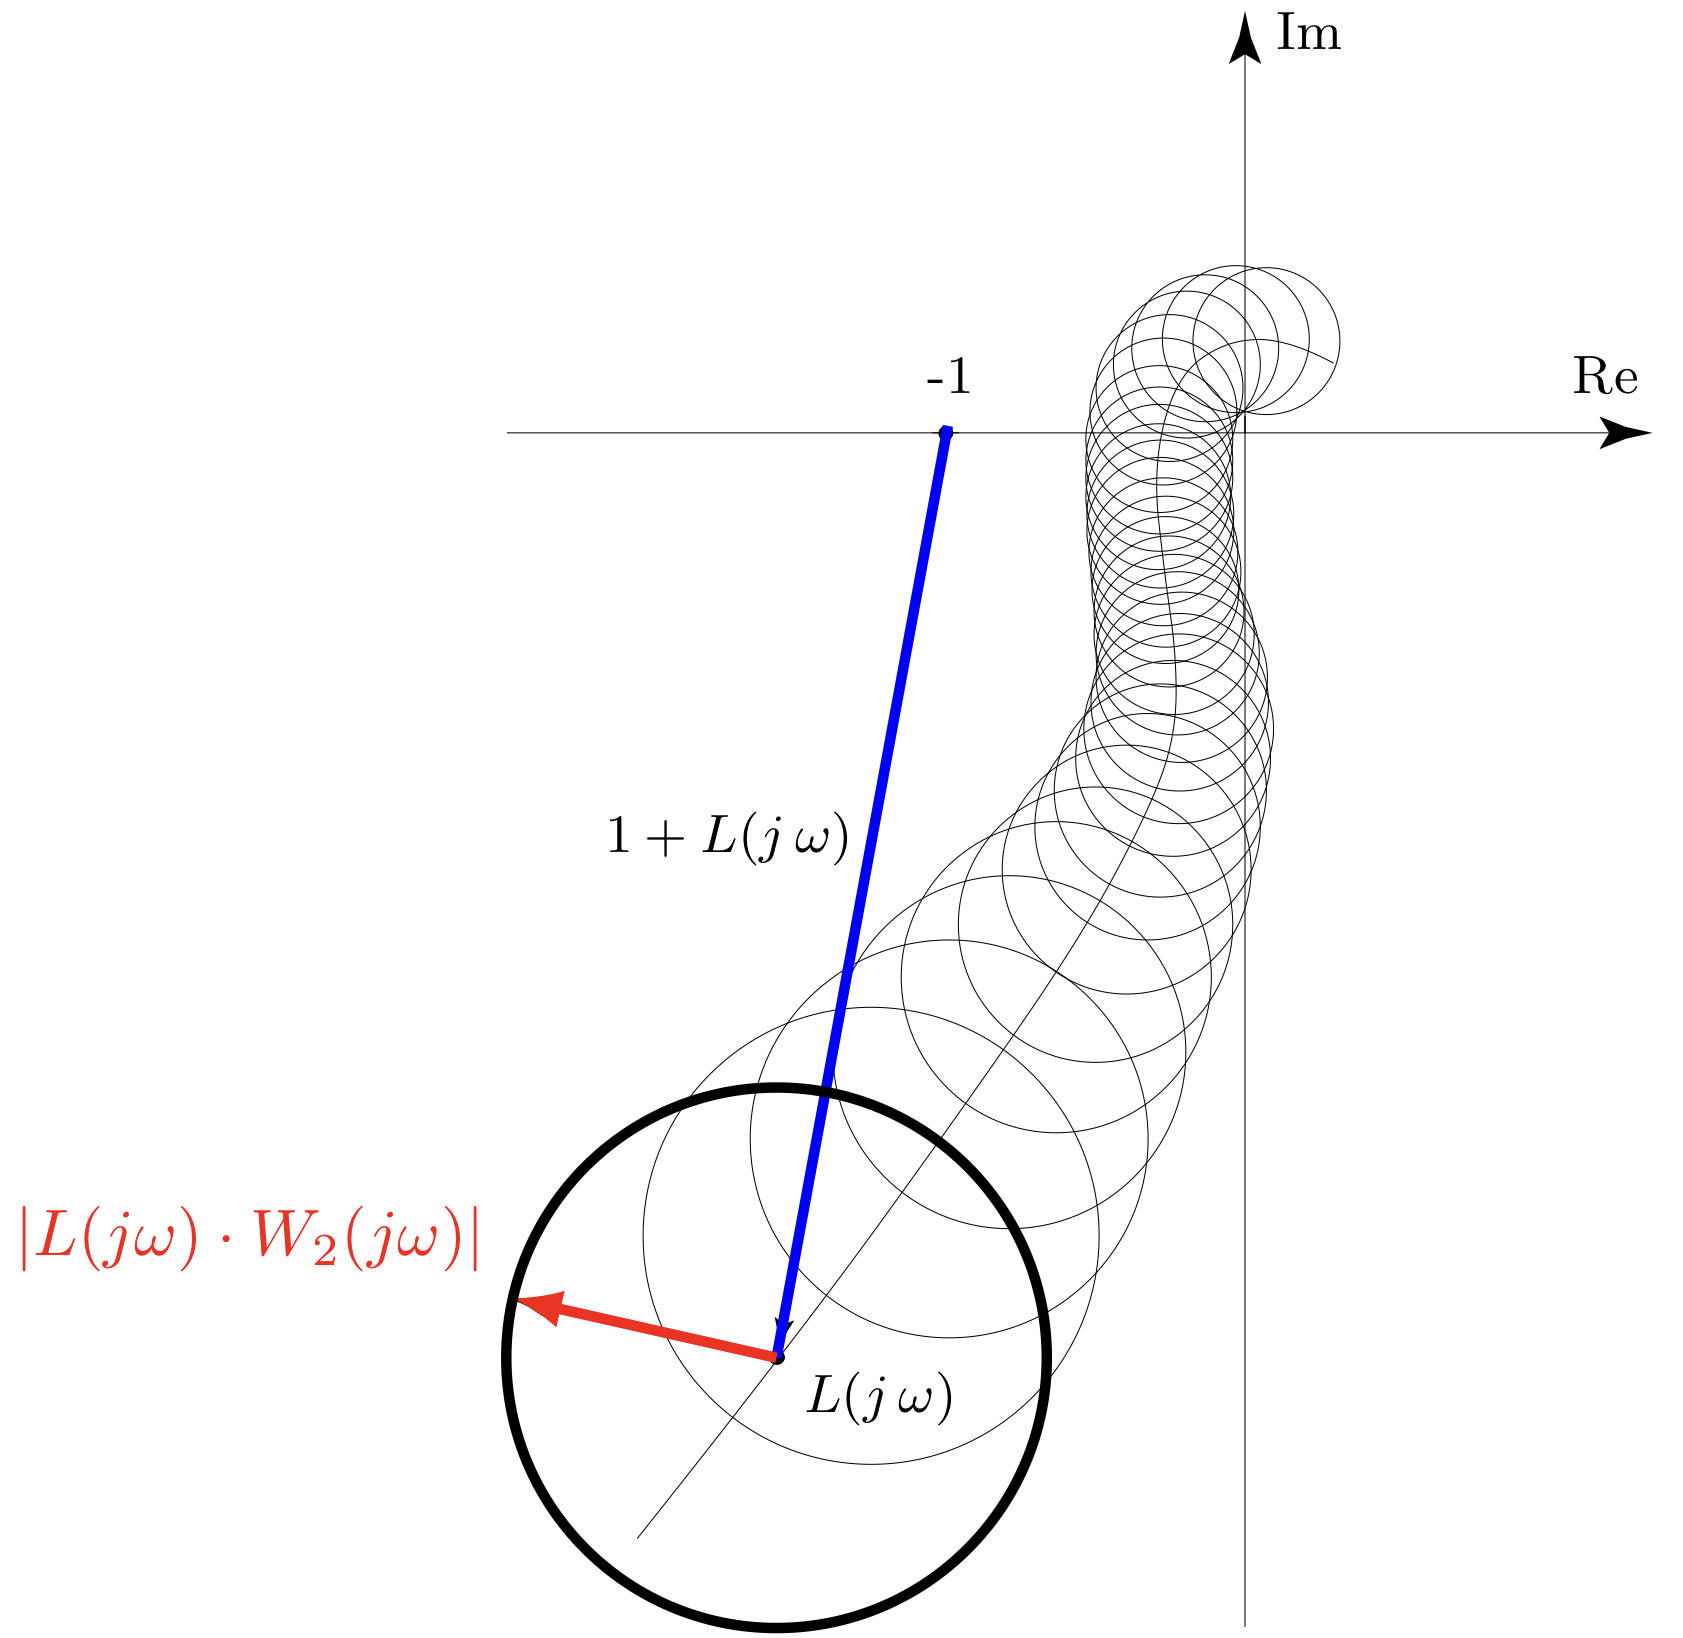
\includegraphics[width= 0.5\linewidth]{03/rob_nyquist.jpeg}
    \end{figure}
    
    Der rote Radius darf nicht grösser werden als der blaue Abstand vom Punkt $(-1 + j0)$ um zusätzliche Umrundungen vom krit. Punkt zu verhindern.
    
\subsection{Multiplikative Spezifikation von \textit{S(s)}}
    Wir wünschen eine betragsmässig kleine Sensitivität um Störungsunterdrückung und gutes reference tracking zu garantieren. Es ist daher sinnvoll den Betrag $|S(s)|$ frequenzabhängig zu limitieren (Disturbances nicht bei allen Frequenzen gleich relevant).
    
    \subsubsection{Nominelle Regelgüte}
        Um die Sensitivität zu Betragsmässig zu begrenzen wird eine rationale TF $W_1(s)$ eingeführt, wobei gelten muss:
        \begin{equation*}
        \colorboxed{red}{
        \begin{aligned}
            \| S(s)\cdot W_1(s)\|_{\textcolor{red}{\infty}} < 1 &\Rightarrow |S(\jw)| < |W_1^{-1}(\jw)|\\
            |W_1(\jw)| &< |1 + L(\jw)|
        \end{aligned}
        }
        \end{equation*}
        
        Die geometrische Interpretation von $W_1(s)$ ist, dass $L(\jw)$ nicht in einen um $(-1 + j0)$ zentrieren Kreis mit Radius $|W_1(\jw)|$ eintreten darf.
    
    \subsubsection{Konstruktion der nominellen Regelgüte}
        $W_1(s)$ kann als Lowpass-Filter konstruiert werden:
        \begin{align*}
            W_1(s) &= k\cdot\frac{\tau\cdot s + 1}{\alpha\cdot\tau\cdot s + 1}, \quad k > 1,\, \alpha > k\\
            \tau^2 &= \frac{k^2 - 1}{\omega_1^2\cdot(\alpha^2-k^2)}, \quad |W_1(\jw_1)| = 1
        \end{align*}
        
        \begin{figure}[H]
            \centering
            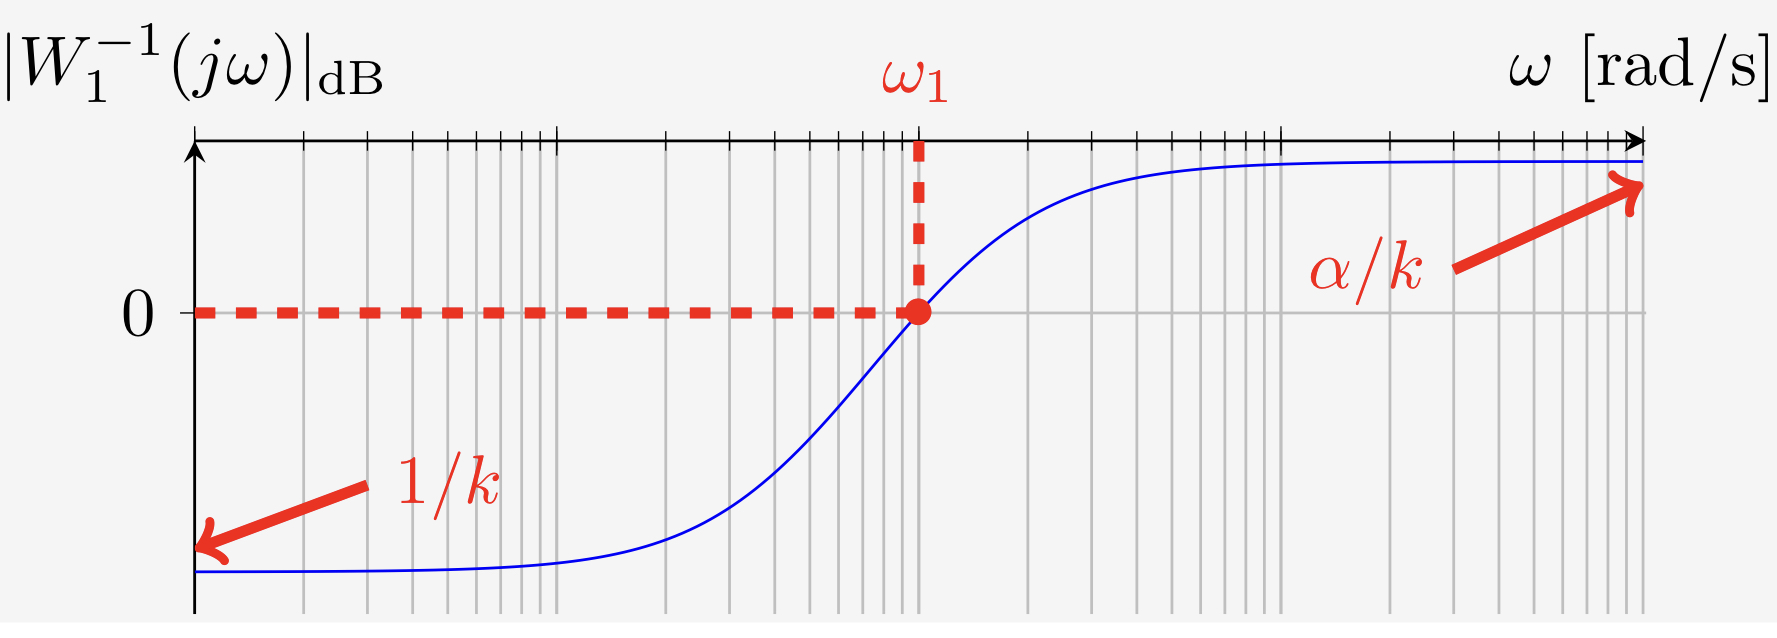
\includegraphics[width = 0.8\linewidth]{images/03/W_1.jpeg}
            \caption{$|W_1^{-1}|_\textnormal{dB}$ in blau. Einstellbare Grössen in rot.}
        \end{figure}


    \input{03_Sensitivity/03_Robuste_Regelgüte}

% \vfill\null\columnbreak    
\section{Kaskadierte Systeme}
    \subsection{Kaskadierte Regelsysteme}
    Kaskadierte Regelsysteme eignen sich für SIMO Systeme mit einer schnellen und einer langsamen Teildynamik. Um die olle Bandbreite der schnellen Dynamik auszunützen werden verschiedene Regler für das schnelle und das langsame Teilsystem ausgelegt.
    
    \begin{figure}[H]
        \centering
        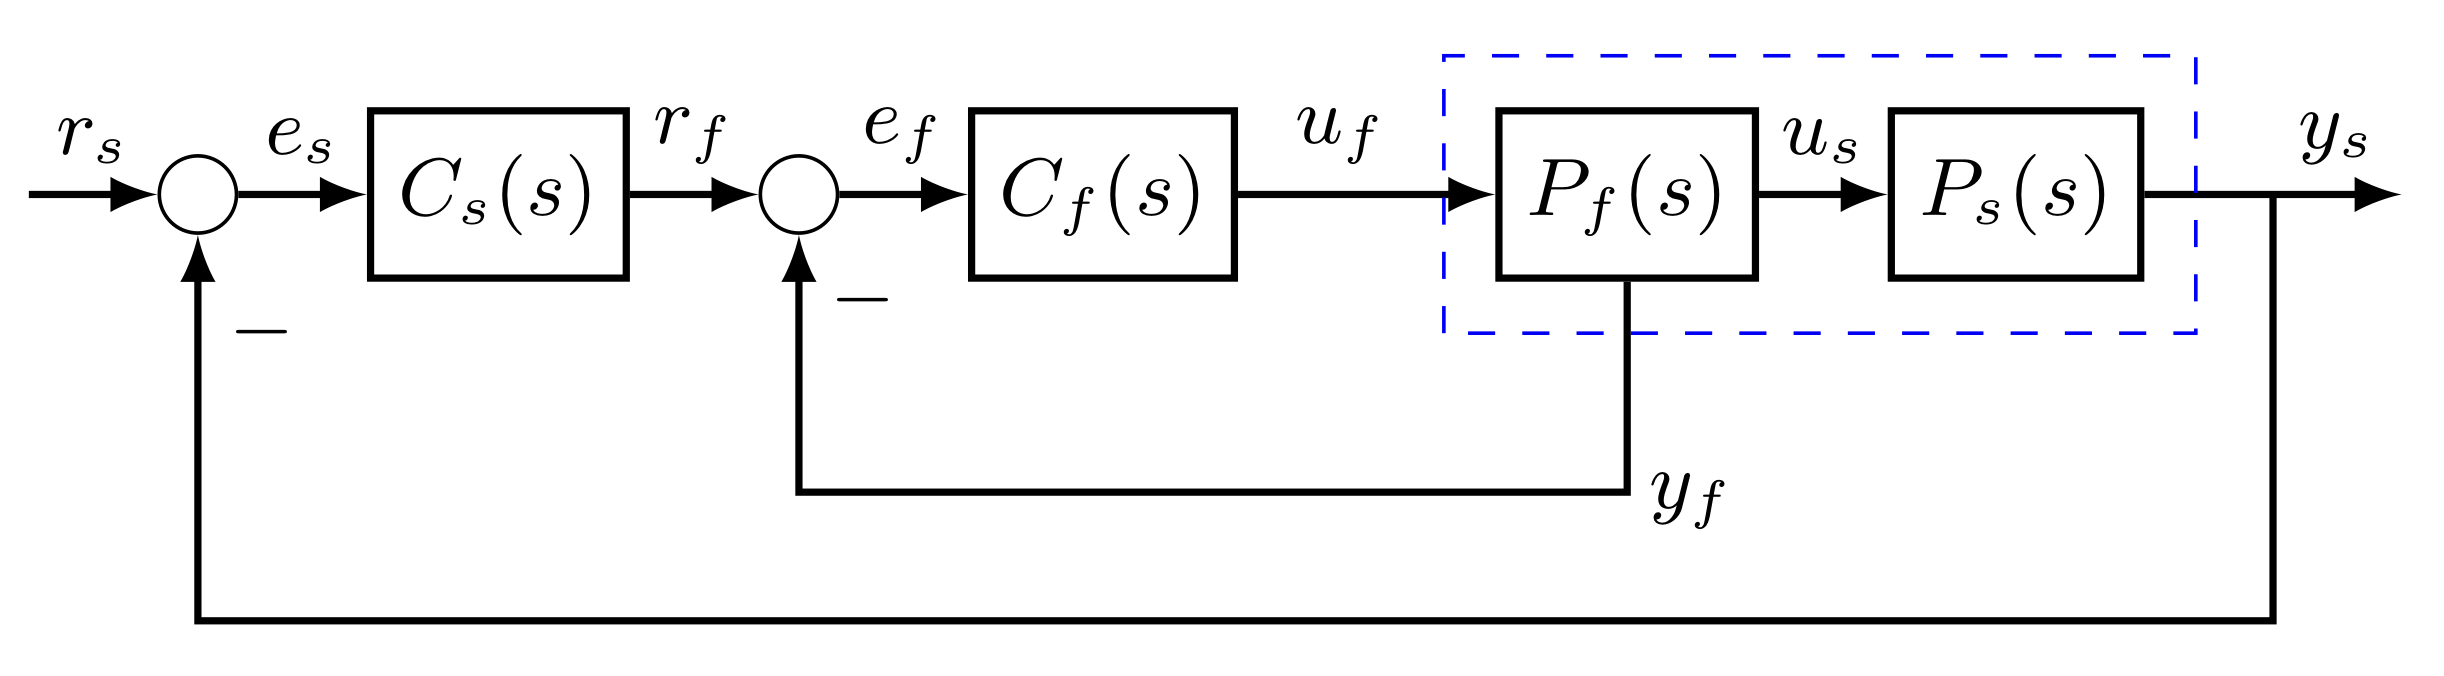
\includegraphics[width = 0.7\linewidth]{images/04/kaskad_sys.jpeg}
        \caption{Kaskadiere Regelstruktur. index $s$ für slow und $f$ für schnell.}
    \end{figure}
    \begin{align*}
        T_{f}(s) &= \frac{L_f(s)}{1 + L_f(s)} = \frac{C_f(s)\cdot P_f(s)}{1 + C_f(s)\cdot P_f(s)}\\
        T_{s}(s) &= \frac{L_s(s)}{1 + L_s(s)} = \frac{C_s(s)\cdot T_{f}(s)\cdot P_s(s)}{1 + C_s(s)\cdot T_f(s) \cdot P_s(s)}
    \end{align*}
    Um die Bandbreite des schnellen Systems auszunutzen wird für $C_f(s)$ oftmals kein Integrator verwendet (verlangsamt). Der Integrator wird in $C_s(s)$ integriert um einen statischen Nachlauffehler zu eliminieren.
    
    \subsubsection{Bsp}
        Masse auf einem Wagen mit einem Feder Dämpfer System an der Wand befestigt.
        \begin{figure}[H]
            \centering
            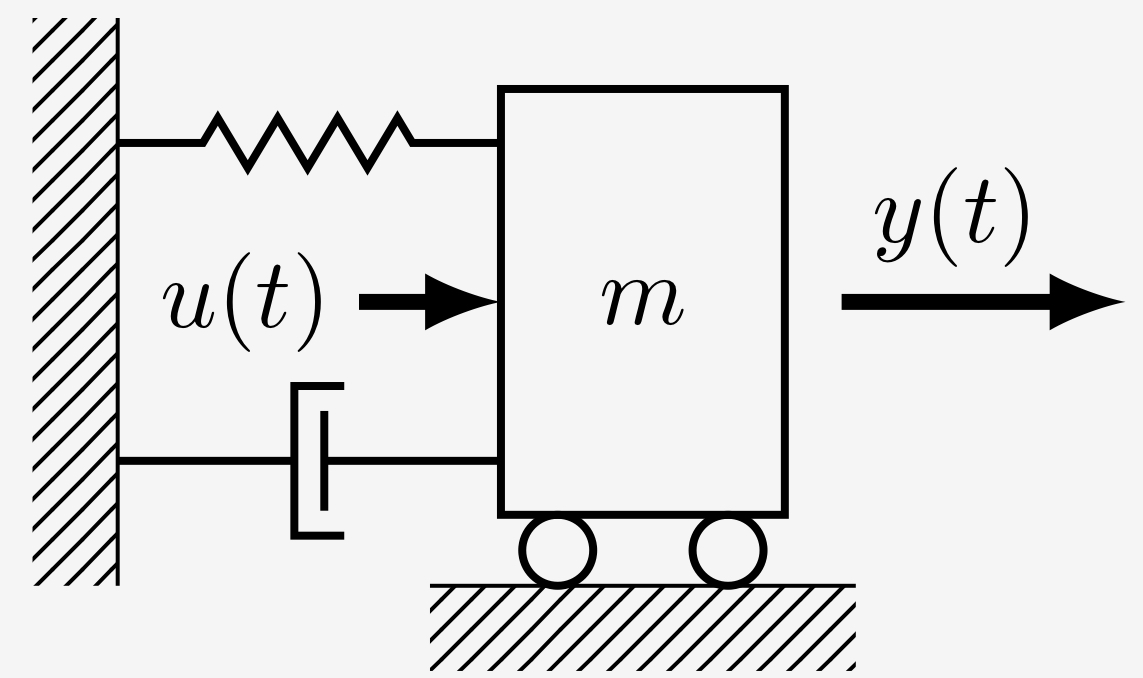
\includegraphics[width = 0.25\linewidth]{images/04/kask_bsp.jpeg}
        \end{figure}
        Man will die Position regeln. Man stellt jedoch fest, dass $u(t)$ direkt auf $v(t)$ wirkt und nur auf indirekt die Position $x(t)$.
        \begin{align*}
            u\rightarrow v: \qquad &P_f(s) = \frac{s}{s^2+s+1}\\
            v\rightarrow x: \qquad &P_s(s) = \frac{1}{s}\\
            u\rightarrow x: \qquad &P(s) = \frac{1}{s^2+s+1}
        \end{align*}
        Auch stellt man fest, dass die Pole von $P_f(s)$ $\pi(P_f(s) = -\frac{1}{2}\pm j\frac{\sqrt{3}}{2}$ einen negativeren Realteil haben als der Pol von $P_s(s)$. \textbf{Pole mit grösserem negativen Realteil klingen schneller ab.}
        
        $P_f$ ist definitiv schneller als $P_s$. Obwohl $\pi(P) =\pi(P_f)$ wird $P_f$ schneller sein, da das System $P$ durch den zusätzlichen offenen Integrator einen grösseren Phasenverlust hat.
        
        Es bietet sich an für $C_f$ einen P-Regler und für $C_s$ einen PI-Regler zu verwenden.

% \vfill\null\columnbreak 
\section{Wurzelortskurven/Root Locus}
    \subsection{Wurzelortskurven/Root locus}
    Mit diesem Verfahren kann man die Pole des geschlossenen Regelkreises setzen wo man will. Man bezeichnet dabei $C(s)$ als Kompensator. Dabei betrachtet man diese Regelstruktur:
    \begin{figure}[H]
        \centering
        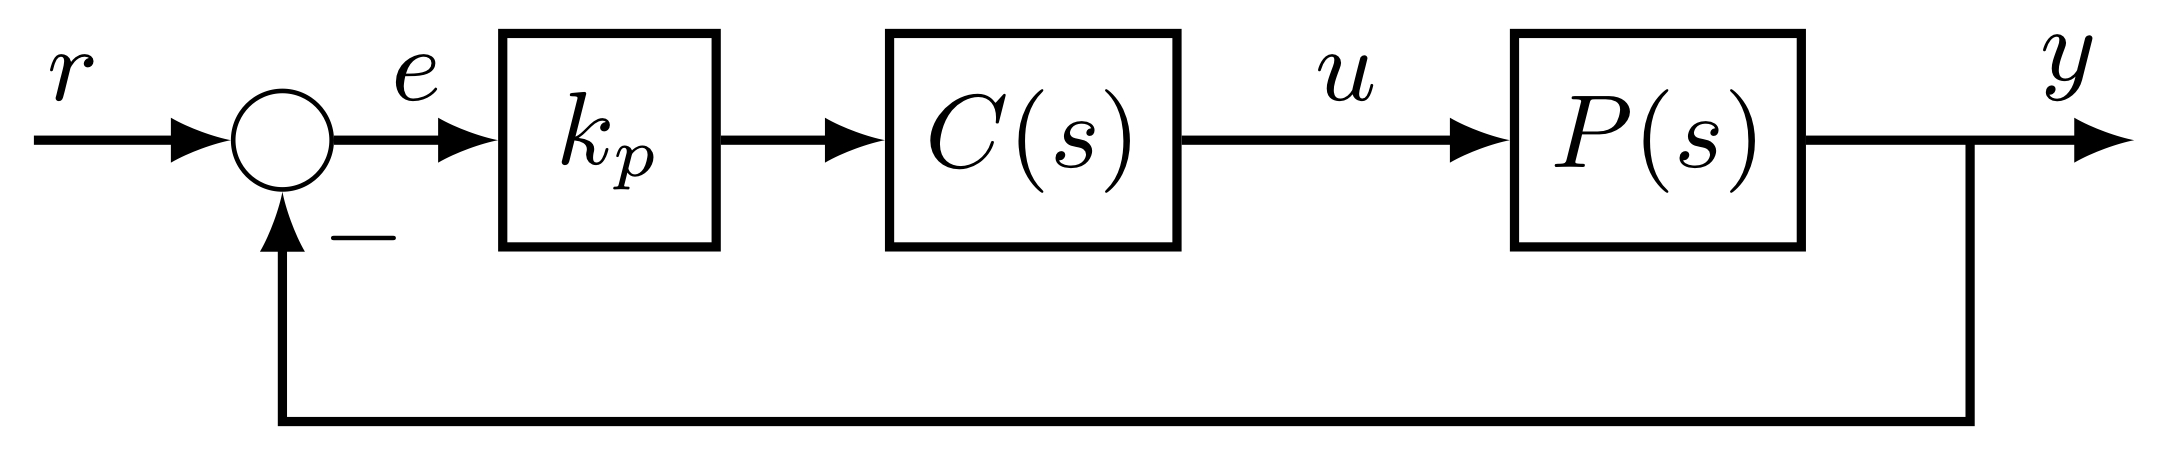
\includegraphics[width = 0.5\linewidth]{images/04/RL_sys.jpeg}
        \caption{Grundstruktur des Root Locus verfahren}
    \end{figure}
    
    $k_p$ wird aus $C(s)$ herausgenommen, da es zu einem freien Parameter wird. Zeichnet man die Pole des geschlossenen Regelkreises für alle $k_p \in(0,\infty)$ erhält man die Wurzelortskurven.
    
    \textbf{Vorsicht!} Wir gehen von einem stabilen, miniphasigen $L(s)$ aus.
    
\subsection{Regeln des Wurzelortskuven-Verfahren}
    Der geschlossene Regelkreis hat folgende TF:
    \begin{equation*}
        T(s) = \frac{k_p\cdot C(s)\cdot P(s)}{1 + k_p\cdot C(s)\cdot P(s)}
    \end{equation*}
    Die Pole von $T(s)$ sind also
    \begin{equation*}
        1 + k_p\cdot L(s) = 0 \quad\textnormal{mit } L(s) = \frac{b(s)}{a(s)} 
    \end{equation*}
    Also gilt:
    \begin{equation*}
        a(s) + k_p\cdot b(s) =: p(s,k_p)
    \end{equation*}
    Die Schar der NST von $p(s,k_p)$ repräsentiert die Wurzelortskurven. Das polynom $p(s,k_p)$ hat Ordnung $n$.
    
    In den Extremfällen gilt:
    
    $\boxed{k_p \rightarrow 0 \Rightarrow p(s,k_p) \approx a(s)}$ Für kleine $k_p$ sind die $n$ NST von $p(s,k_p)$ die $n$ NST von $a(s)$ $\Rightarrow$ die Pole von $T(s)$ nähern sich den Polen von $L(s)$.
    
    $\boxed{k_p \rightarrow \infty \Rightarrow p(s,k_p) \approx k_p\cdot b(s)}$ Für sehr grosse $k_p$ konvergieren $m$ NST von $p(s,k_p)$ zu den $m$ endlichen NST von von $b(s)$. $\Rightarrow$ Die Pole von $T(s)$ nähern sich den NST von $L(s)$. Jedoch hat $p(s,k_p)$ Ordnung $n$. Dh. es bleiben $n-m$ NST von $p(s,k_p)$ übrig. Diese divergieren zu $\infty$. (Reminder: NST im unendlichen beeinflussen Systemdynamik nicht)
    
    \subsubsection{Vorgehen}
        \begin{enumerate}
            \item Ursprung der Asymptoten berechnen:
                \begin{equation*}
                    \sigma_a = \frac{1}{n-m}\left( \sum_{i=1}^n \operatorname{Re}(\pi_i) - \sum_{i=1}^m \operatorname{Re}(\zeta_i) \right)
                \end{equation*}
                die Asymptoten verlassen den  Punkt $(\sigma_a + j\cdot 0)$.
                
            \item Winkel der Asymptoten bestimmen:
                \begin{equation*}
                    \delta_i = \frac{\pi}{n-m}\cdot(2\cdot(i-1)+1)[\textnormal{rad}],\quad i = 1,\dots,n-m
                \end{equation*}
        \end{enumerate}
        
        Man kann testen ob ein Punkt $z\in\mathbb{C}$ auf der Wurzelortskurven liegt, indem man ihn in diese Gleichung einsetzt:
        \begin{equation*}
        \colorboxed{red}{
            \sum_{i=1}^m \angle(z-\zeta_i) - \sum_{i=1}^n \angle (z-\pi_i) \overset{!}{=} -\pi \pm 2\pi \cdot k,\quad k\in\mathbb{N}
            }
        \end{equation*}
    
    \subsubsection{Skizzierhilfen}
        \begin{itemize}
            \item Root Locus ist Symmetrisch zur Re-Achse.
            \item Treffen sich 2 Pole, dann drehen beide sich um $90^\circ$ in der komplexen Ebene.
            \item Alle Pkte auf der Re-Achse links von einer ungerade Anzahl $\pi\, \&\, \zeta$ sind mögliche $\pi_{T(s)}$.
            \item $r=n-m$ Pole divergieren entlang gerader Asymptoten ins unendliche.
        \end{itemize}
    
    \subsubsection{Bsp}
        \begin{equation*}
            L(s) = \frac{s+4}{(s+1)(s+2)(s+3)}
        \end{equation*}
        $\rightarrow\, n=3,\, m=1,\, n-m=2$. Wir wissen also, dass 2 Pole sich für $k_p \rightarrow \infty$ den Asymptoten, welche bei $(\sigma_a +j\cdot 0)$ und steigung $\delta_i$ haben, annähern.
        \begin{align*}
            \sigma_a &= \frac{1}{2}\big(-1-2-3-(-4)\big) = -1\\
            \delta_1 &= \frac{\pi}{2}\big(2\cdot0 + 1\big) = \frac{\pi}{2}, \quad \delta_2 = \frac{\pi}{2}\big(2\cdot(2-1) + 1\big) = \frac{3\pi}{2}
        \end{align*}
        
        Die Wurzelortskurven sind also:
        \begin{figure}[H]
            \centering
            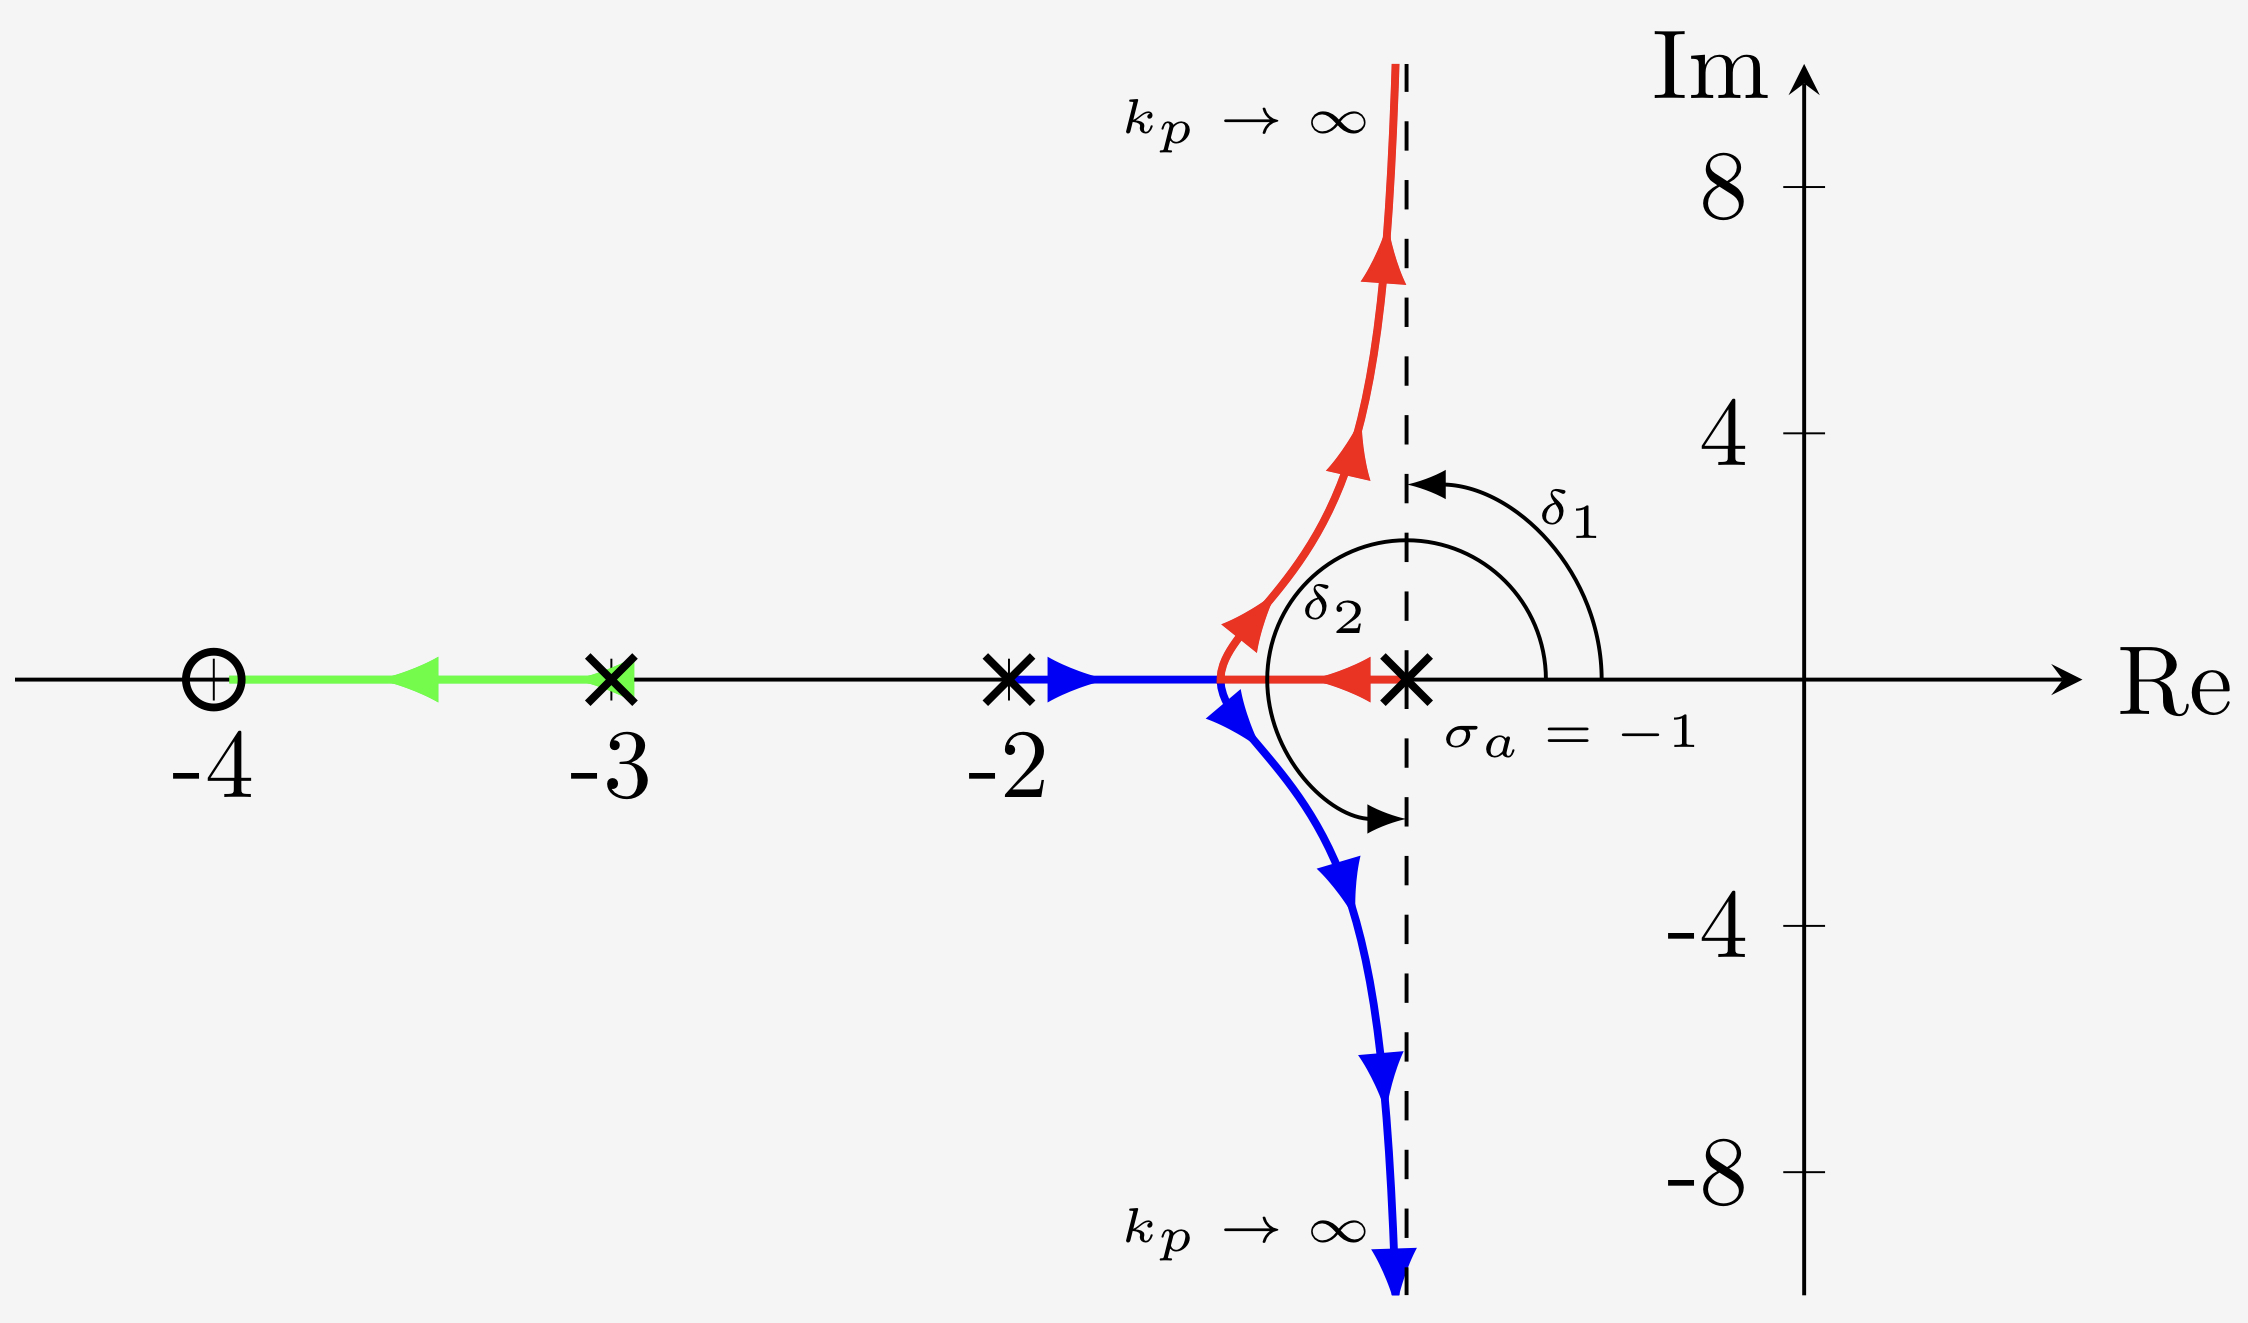
\includegraphics[width= 0.6\linewidth]{images/04/RL_bsp.jpeg}
        \end{figure}
       \textbf{Achtung: } Pole kennzeichnet man mit $\mbox{\Large$\times$}$ und NST mit $\bigcirc$ 
       
       Ist $(-3.5+j\cdot0)$ auf den WOK?
       \begin{gather*}
           \angle(-3.5+4) - \big(\angle(-3.5+1) + \angle(-3.5+2) + \angle(-3.5+3)\big)= 0 - 3\pi\\ \rightarrow k = 2 \in \mathbb{N} \quad\checkmark
       \end{gather*}
       
\subsection{Kompensierung mit Wurzelortskurven}    
    Man kann mit dem Zugehörigskeitstest einen Kompensator/Regler finden, den die Pole des geschlossenen Regelkreises an einen gewünschten Ort bringt.
    
    \subsubsection{Bsp}
        \begin{equation*}
            P(s) = \frac{1}{(s+1)(s+3)}
        \end{equation*}
        Wir wollen Pole von T(s) bein $s^*_{1,2} = -4 \pm j\cdot4$ rad/s. Wir testen zuerst einen einfachen Kompensator $C_1(s) = 1$, stellen aber fest, dass die gewünsten Pole (\Large$\textcolor{red}{\times}$\normalsize)  nicht auf den WOK liegen. Dh es existiert für $C_1(s)$ kein $k_p$ für dass die gewünschten Pole platziert werden.
        
        \begin{figure}[H]
            \centering
            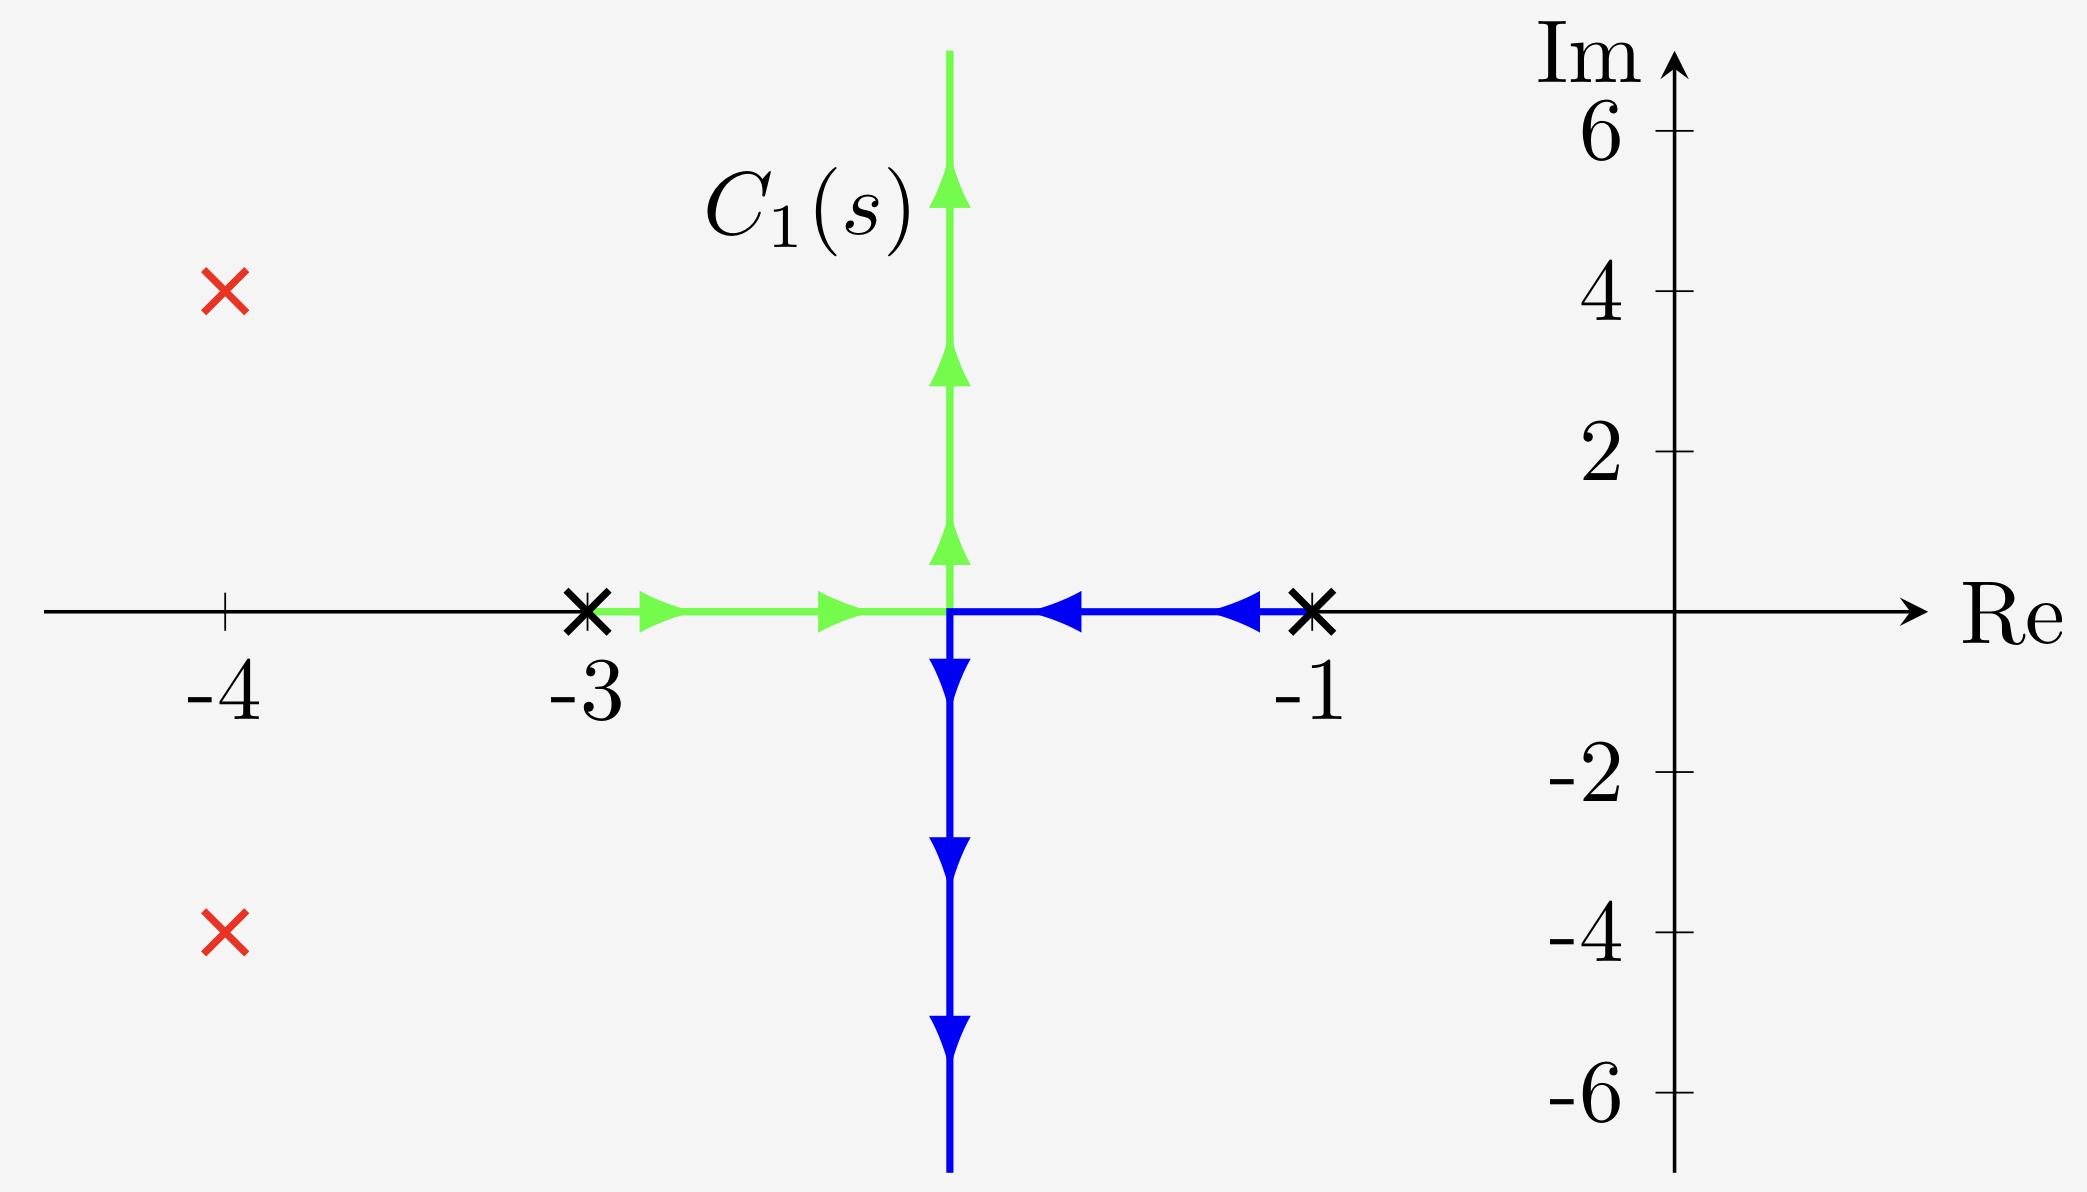
\includegraphics[width = 0.5\linewidth]{images/04/RL_kom_bsp1.jpeg}
            \caption{WOK von $C_1(s)=1$}
        \end{figure}
        
        Die Pole Liegen Links der WOK. Um die WOK nach links zu biegen nehmen wir mit $C_2(s) = s + \zeta$ eine parametrisierte NST als Kompensator.
        
        \begin{figure}[H]
            \centering
            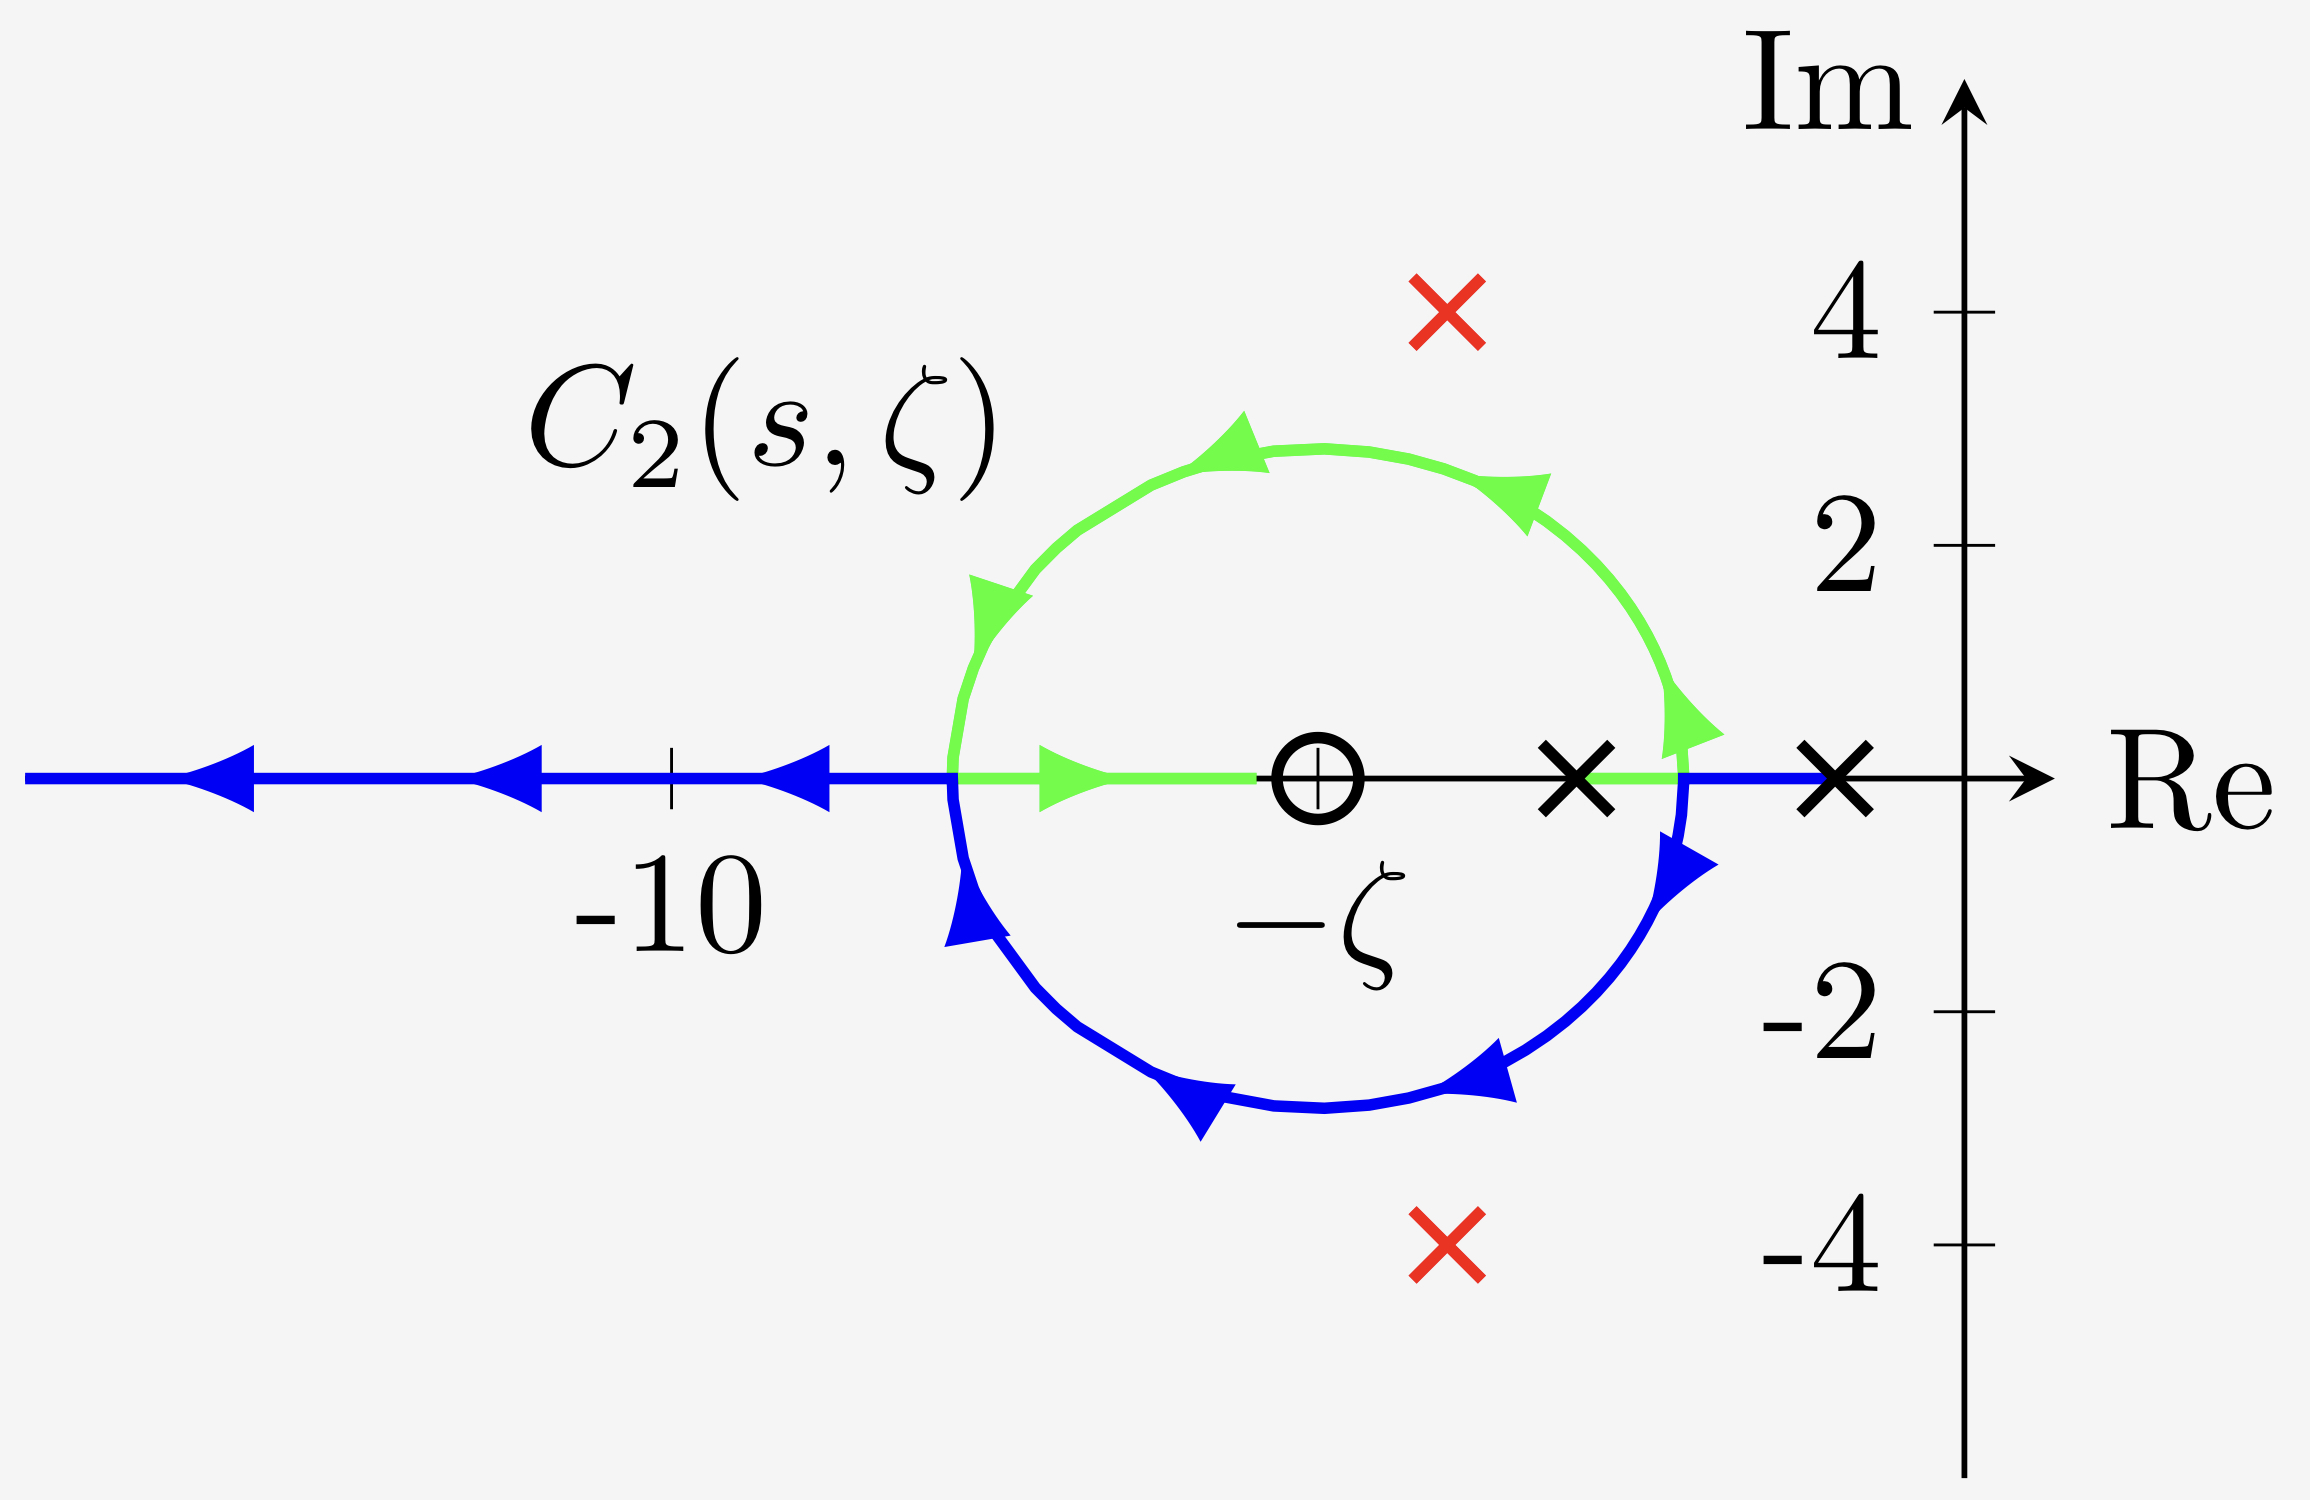
\includegraphics[width = 0.5\linewidth]{images/04/RL_kom_bsp2.jpeg}
            \caption{WOK von $C_2(s)=1$}
        \end{figure}
        
        Um $\zeta$ zu finden benutzen wir den Test ob ein Punkt auf den WOK ist:
        \begin{gather*}
            L(s) = \frac{s+\zeta}{(s+1)(s+3)} \angle L(s) = \angle(s+\zeta) -\angle(s+1)-\angle(s+3)\\
            \xrightarrow{s = s^*}  \angle(-4+4j+\zeta) -\angle(-4+4j+1)-\angle(-4+4j+3) = \\
            \underbrace{\arctan\left(\frac{4}{\zeta-4}\right)}_\gamma-\underbrace{\arctan\left(\frac{4}{-3}\right)}_\alpha - \underbrace{\arctan\left(\frac{4}{-1}\right)}_\beta \overset{!}{=} -\pi\\
            \Rightarrow \gamma = -\pi+\alpha+\beta \Leftrightarrow \zeta = 4 + \frac{4}{\tan\gamma} \approx 7.25\textnormal{ rad/s}
        \end{gather*}

\vfill\null\columnbreak 
\section{PID in der Praxis}
    \subsection{Set point Weights}
        Mit den set point weights kann das Regelverhalten verbessert werden. Dabei wird die Referenz $r(t)$ seperat mit einer Verstärkung ($a,\, b,\, c$) multipliziert.
        
        \begin{figure}[H]
            \centering
            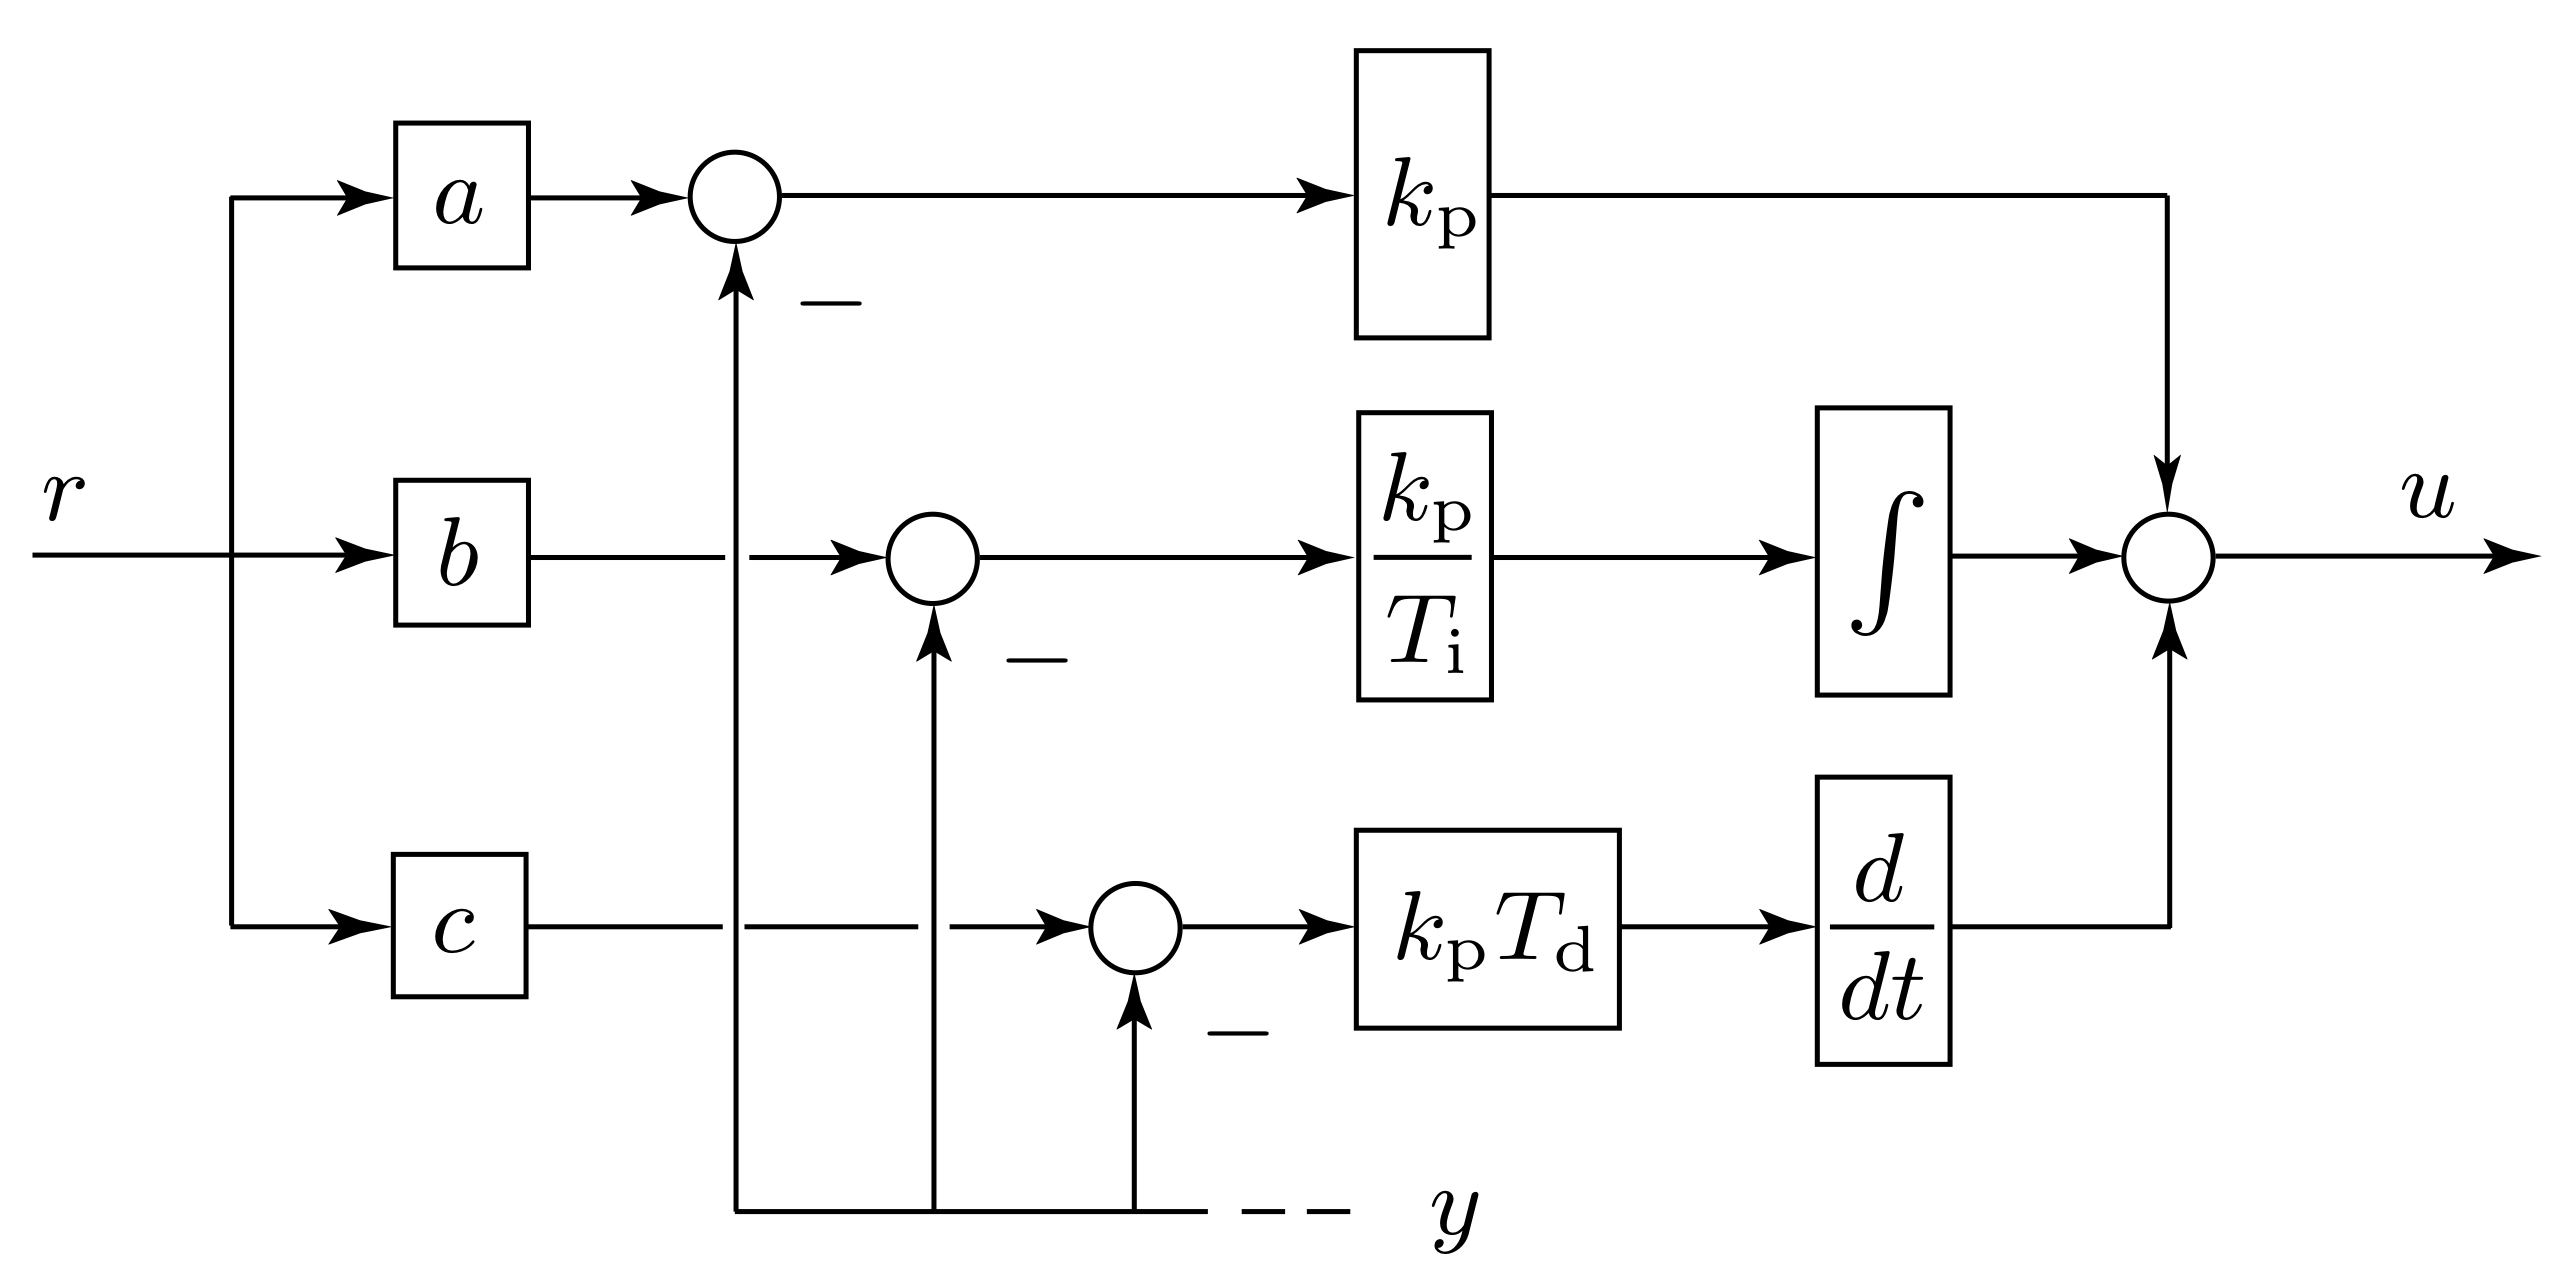
\includegraphics[width = 0.5\linewidth]{images/04/spw.jpeg}
        \end{figure}
        
        \begin{itemize}
            \item $b=1$ um einen statischen Nachlauffehler zu verhindern falls die Referenz möglichst konstant werden soll.
            
            \item $c=0$ Normalerweise will man nur Änderungen aufgrund des Ausgangssignals dämpfen. Ein Step in $r(t)$ würde auf dem Differential-Pfad zu einem Dirac-Stoss führen.
            
            \item $a$ wird mit \r{A}ström-Hägglund bestimmt. Typischerweise wählt man $a\in(0,1)$. Ein guter Wert für $a$ verbesert häufig das closed-loop Verhalten.
        \end{itemize}
        \textbf{Bemerkung:} Die Gewichtungen Beeinflussen die Stabilität des geschlossenen Reglekreises \textbf{nicht!}
        \begin{equation*}
            T(s) = \frac{Y(s)}{R(s)}\frac{P\cdot\overbrace{\Big(a\cdot k_p +b\cdot\frac{k_p}{T_i\cdot s} + c\cdot k_p\cdot T_d\cdot s\big)}^{C_{\textnormal{PID,weighted}}}}{1 + P\cdot\underbrace{\Big(k_p + \frac{k_p}{T_i\cdot s} + k_p\cdot T_d\cdot s\big)}_{C_{\textnormal{PID,unweighted}}}}
        \end{equation*}
    \subsection{Saturation und Anti Reset Windup (ARW)}
    Eine Saturation ist eine Nichtlinearität, die in allen technischen Systemen vorhanden ist, da Aktuatoren nie beliebig kleine/grosse Sollsignale $u(t)$ umsetzen können.
    \begin{equation*}
        \Bar{u}(t) = 
        \begin{cases}
        u_\textnormal{min}   &\textnormal{if } u(t) < u_{\textnormal{min}}\\
        u_\textnormal{max}   &\textnormal{if } u(t) > u_{\textnormal{max}}\\
        u(t)    &\textnormal{else}
        \end{cases}
    \end{equation*}
    % Falls der vom Regler $C(s)$ geforderte Ausgang $u(t)$ grösser ist als der maximal produzierbare Eingang $u_{\textnormal{max}}$ des Aktuators, saturiert der Eingang bei $\Bar{u}(t) = u_{\textnormal{max}}$. Analog für den minimalen Eingang.
    \begin{figure}[H]
        \centering
        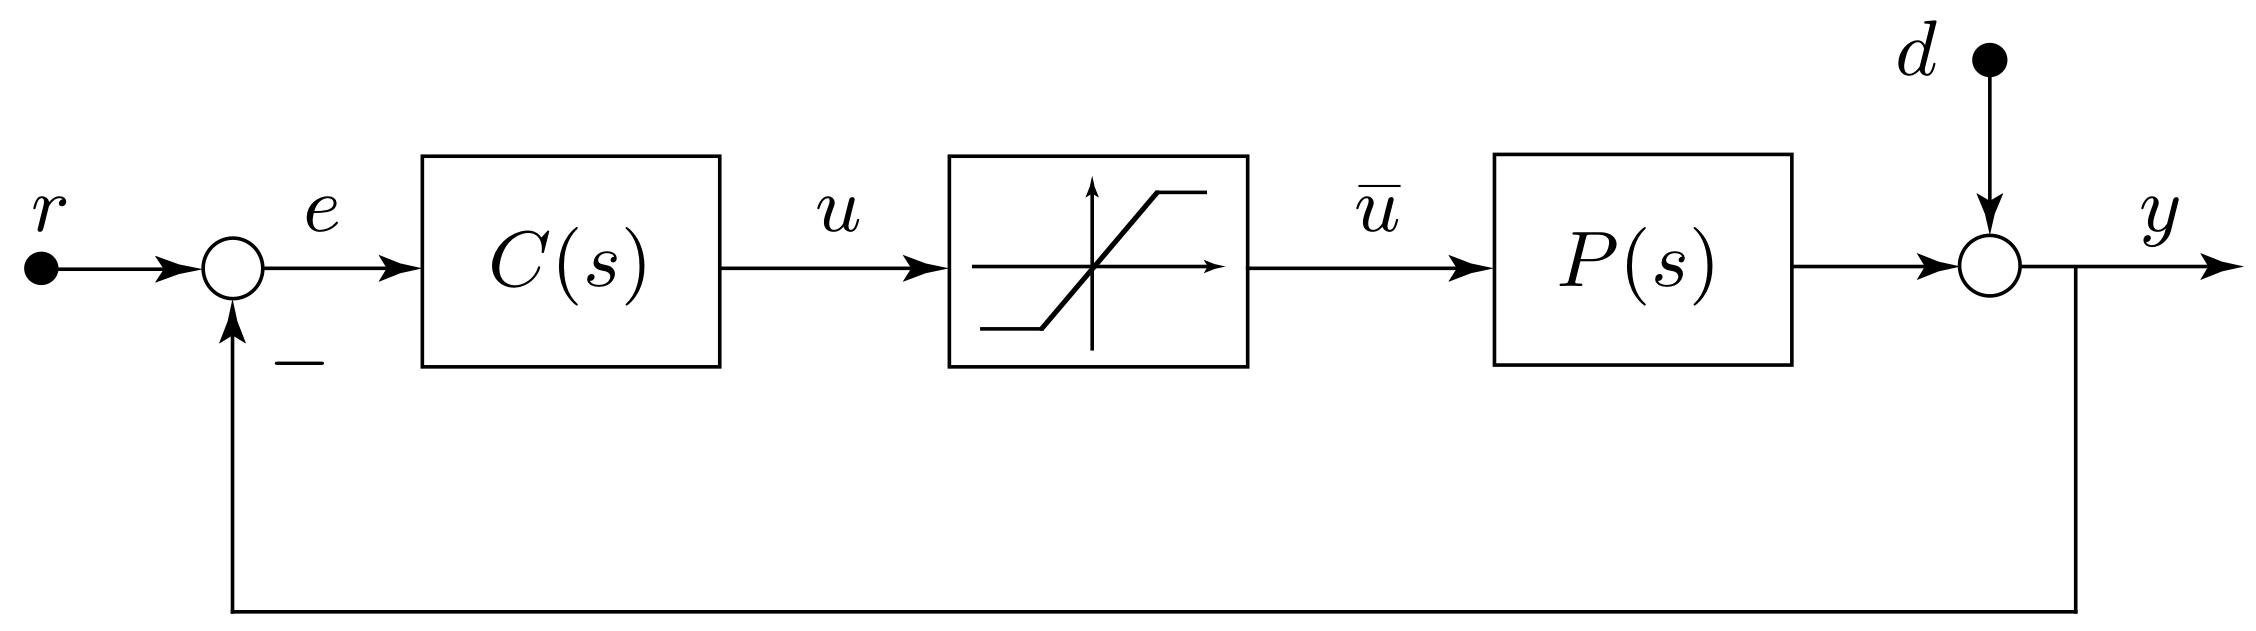
\includegraphics[width = 0.6\linewidth]{images/04/arw.jpeg}
    \end{figure}
    
    Wie kommt es zu Saturation? Da das System langsamer reagiert als man erwartet, haben Integratoren mehr Zeit um sich zu füllen. Sobald dann aber das Vorzeichen des Fehlers ändert Überschiesst der Regler zuerst das Ziel, da sich der Integrator zuerst wieder Entleeren muss um eine Änderung im Aktuatorsignal hervorzurufen. 
    
    \subsubsection{ARW/Bumpless Transfer}
        Um diese Saturation zu verhindern, wird der Integrator um ein \textit{Anti-Reset Windup} (ARW) erweitert, der das ``überfüllen" des Integrators verhindert. Dazu wird die differenz $q(t) = u(t) - \Bar{u}(t)$ vom Integrator abgezogen. Falls $u(t)$ nicht saturiert, ist $q(t)= 0$.
        
        Meist ist es sinvoll, nebst einem Automatischen Modus, einen Manuellen Modus für die Steuerung des Systems zu haben. Möchte man von einem Modus in den Anderen wechseln, so soll das so rebungslos/smooth wie möglich passieren, um Stösse auf das System zu verhindern. Dazu verwendet man den \textit{Bumpless Transfer}.
        
        \begin{figure}[H]
            \centering
            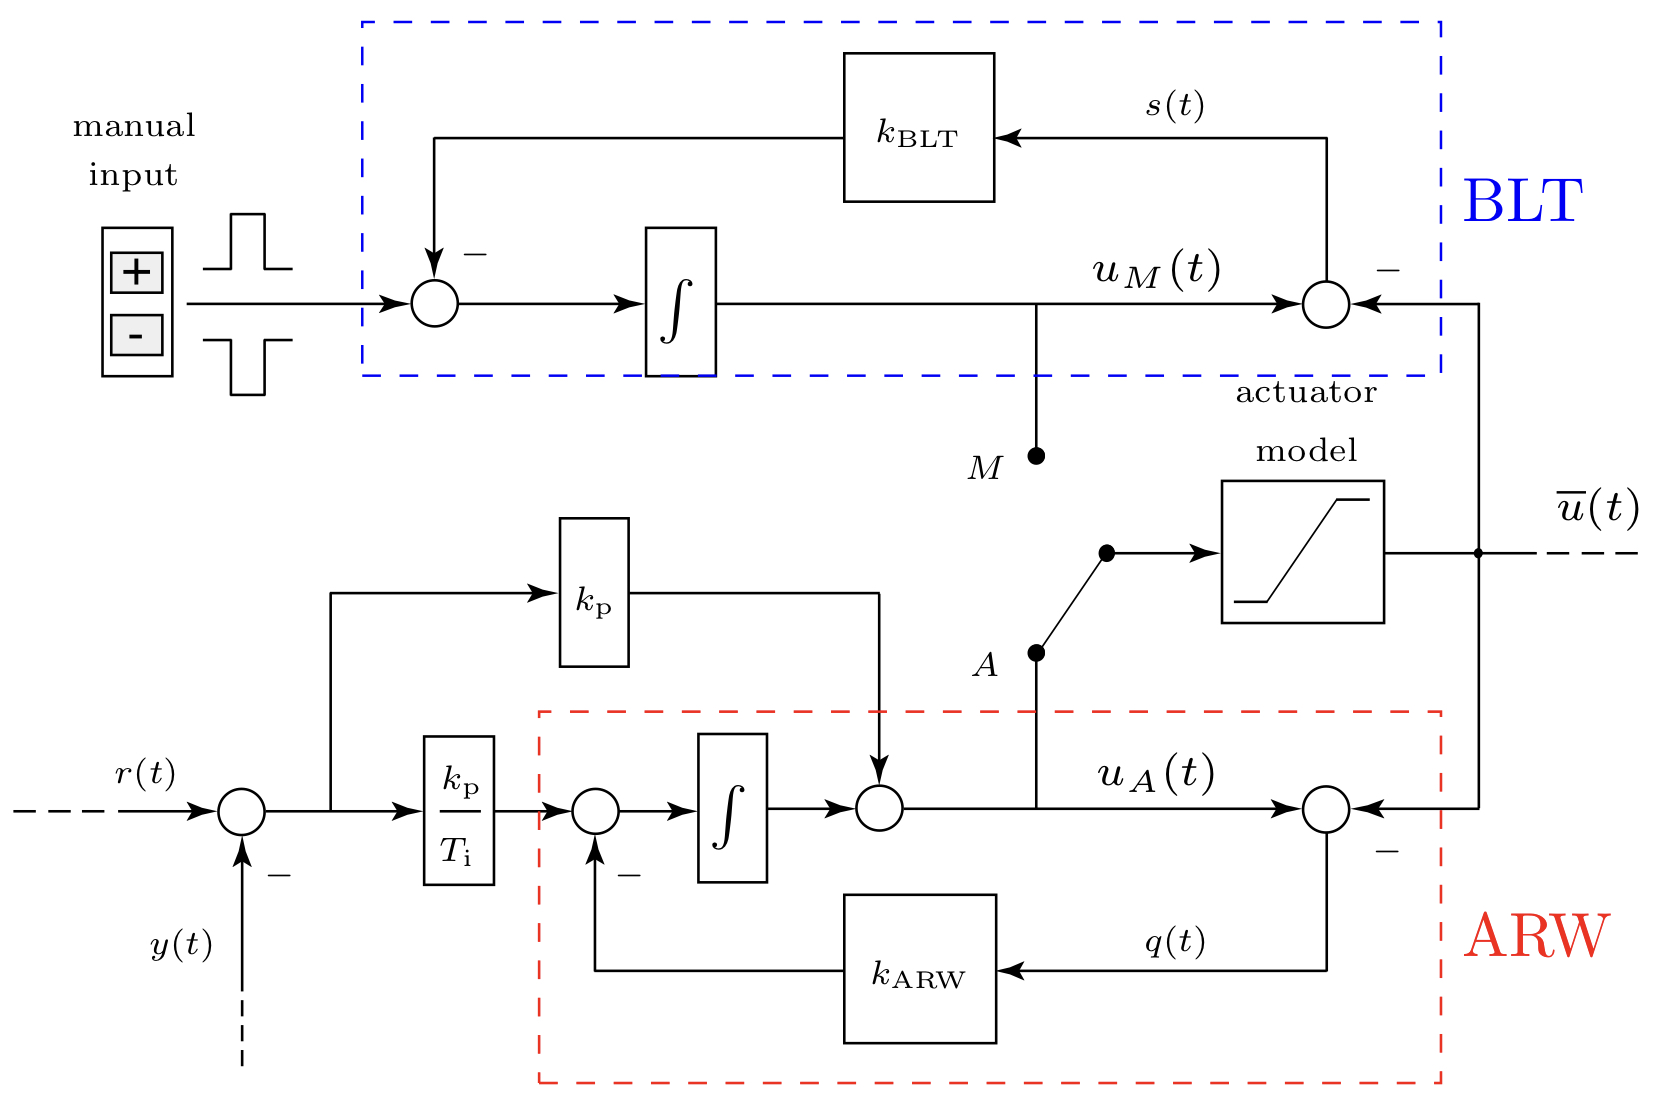
\includegraphics[width = 0.8\linewidth]{images/04/arw_bt.jpeg}
            \caption{Realisation von ARW und BLT}
        \end{figure}
        
    \subsubsection{Bsp}
        Für ein System wurde ein PI-Regler ausgelegt und das resultierende System wurde simuliert. Man stellt fest, dass die Perfomance ohne ARW schlechter ist, als mit ARW.
        
        \begin{figure}[H]
            \centering
            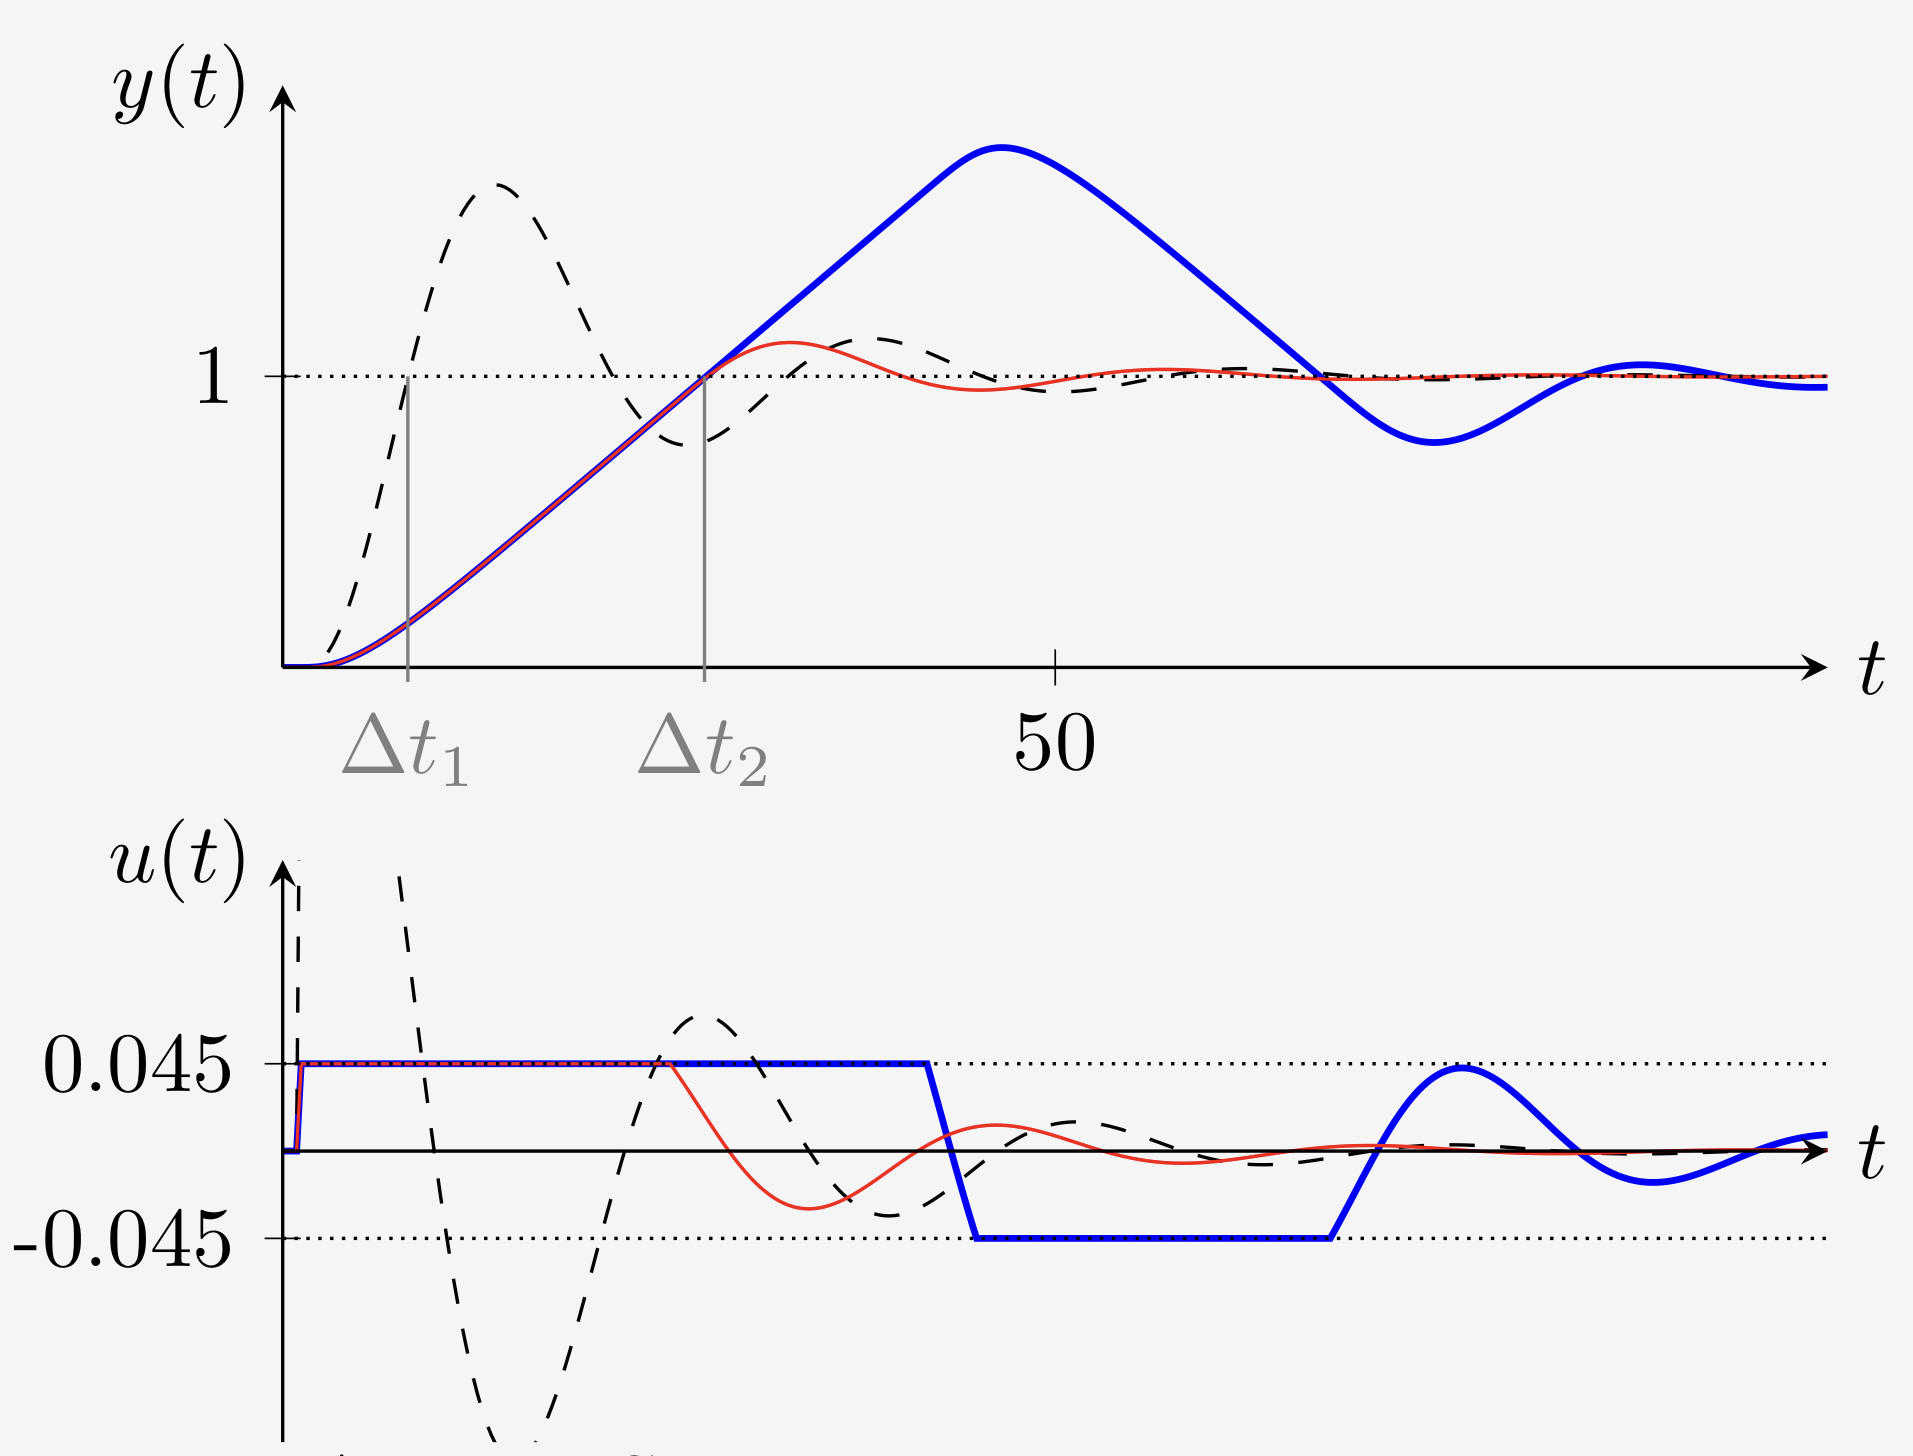
\includegraphics[width = 0.6\linewidth]{images/04/arw_bsp.jpeg}
            \caption{\textcolor{blue}{Blau: system ohne ARW}, \textcolor{red}{Rot: system mit ARW} und Dashed: Ideales System ohne Saturation}
        \end{figure}
    \subsection{Gain Scheduling}
    Bei nichtlinearen Systemen will man meist um verschiedene Betriebspunkte linearisieren. Dafür braucht es bei jedem Betriebspunkt einen anderen linearen Regler. Bei einem PI-Regler werden $k_p(o),\, T_i(o)$ zu Funktionen des Betriebspunktes $o$.
    
    \begin{figure}[H]
        \centering
        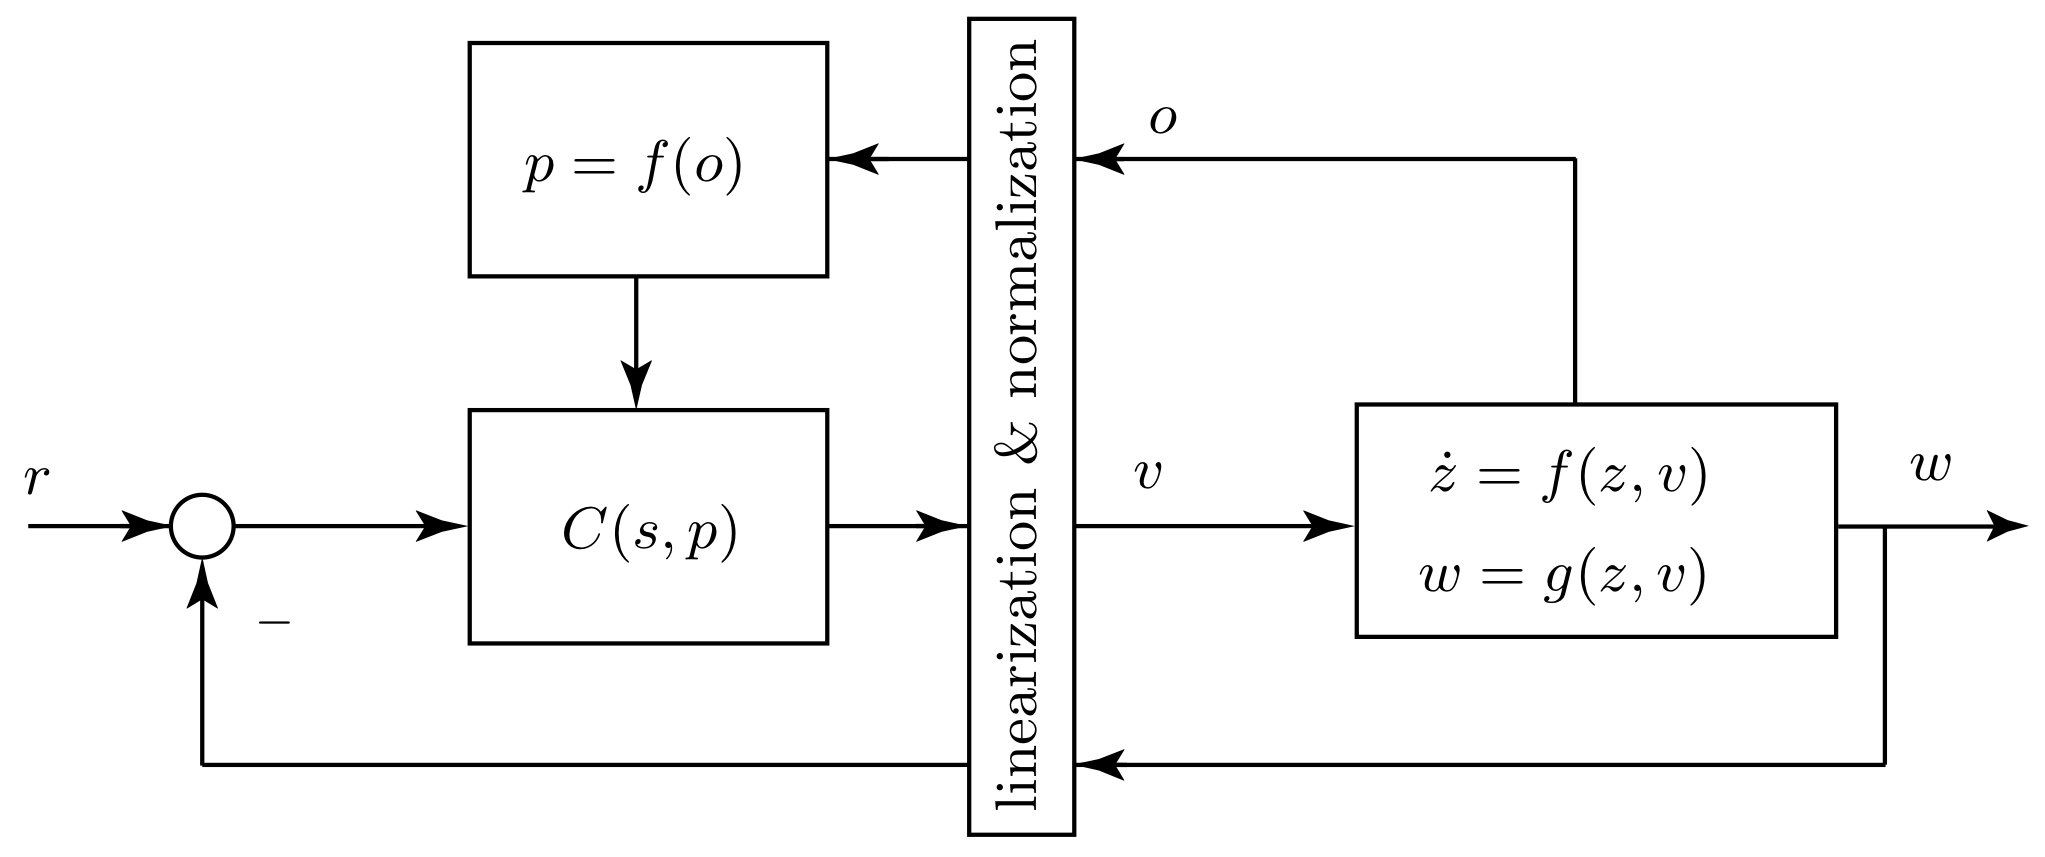
\includegraphics[width = 0.6\linewidth]{images/04/gain_sched.jpeg}
        \caption{Diagramm zu Gain scheduling}
    \end{figure}
    
\subsection{Analoge Realisierung}
    In manchen Anwendungen macht es Sinn, den Regler durch analoge Schaltungen anstatt durch Software zu realisieren. Mit diesen kann man eine Eingangsspannung $U_e$ in eine Ausgangsspannung $U_a$ umwandeln. Dabei kann man folgender Grundstruktur folgen:
    
    \begin{figure}[H]
        \centering
        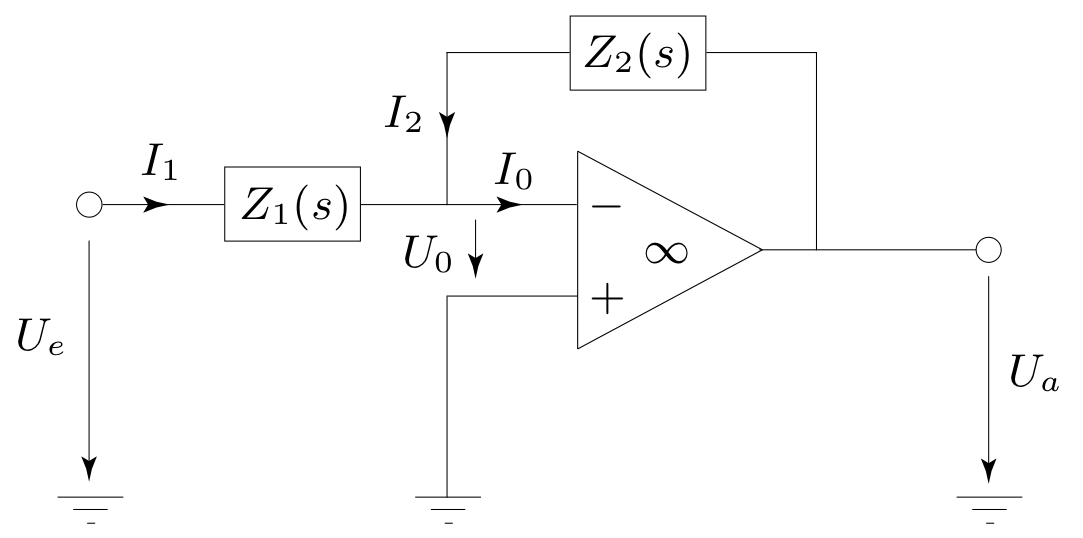
\includegraphics[width = 0.5\linewidth]{images/04/analog_real.jpeg}
        \caption{Grundstruktur analoge Realisierung mit einem idealen Op-Amp}
    \end{figure}
    
    Die Übertragungsfunktion lautet dabei
    \begin{equation*}
        \Sigma(s) = \frac{U_a(s)}{U_e(s)} = -\frac{Z_2(s)}{Z_1(s)}
    \end{equation*}
    
    Dabei konstruiert man $Z_1(s),\, Z_2(s)$ aus Widerständen ($R$), Induktoren ($L$) und Kapazitäten ($C$)
    \begin{equation*}
        Z_r(s) = R, \qquad Z_L(s) = s\cdot L, \qquad Z_c(s) = \frac{1}{s\cdot C}
    \end{equation*}
    
    Die Kirchhoffschen Reglen für Serie- und Parallelschaltungen von Elementen helfen bei der Realisierung der TF.
    
\subsection{Zeitdiskrete Realisierung}
    Da ein Regler, der auf Software basiert nur bei einer fixen Taktfrequenz $\mathit{f}_s$ an diskreten Stellen den Regel auswerten kann, muss man einen continuous-time Regler $C(s)$ ind einen discrete-time Regeler $C(z)$ umwandeln. Es können nur an fixen Zeitpunkten $t_n$ neue eingänge $u(n\cdot T_s):=u[k]$ berechnet werden:
    \begin{equation*}
        t_n = \frac{n}{\mathit{f}_s} = n\cdot T_s,\, n\in0,1,\dots
    \end{equation*}
    
    \begin{figure}[H]
        \centering
        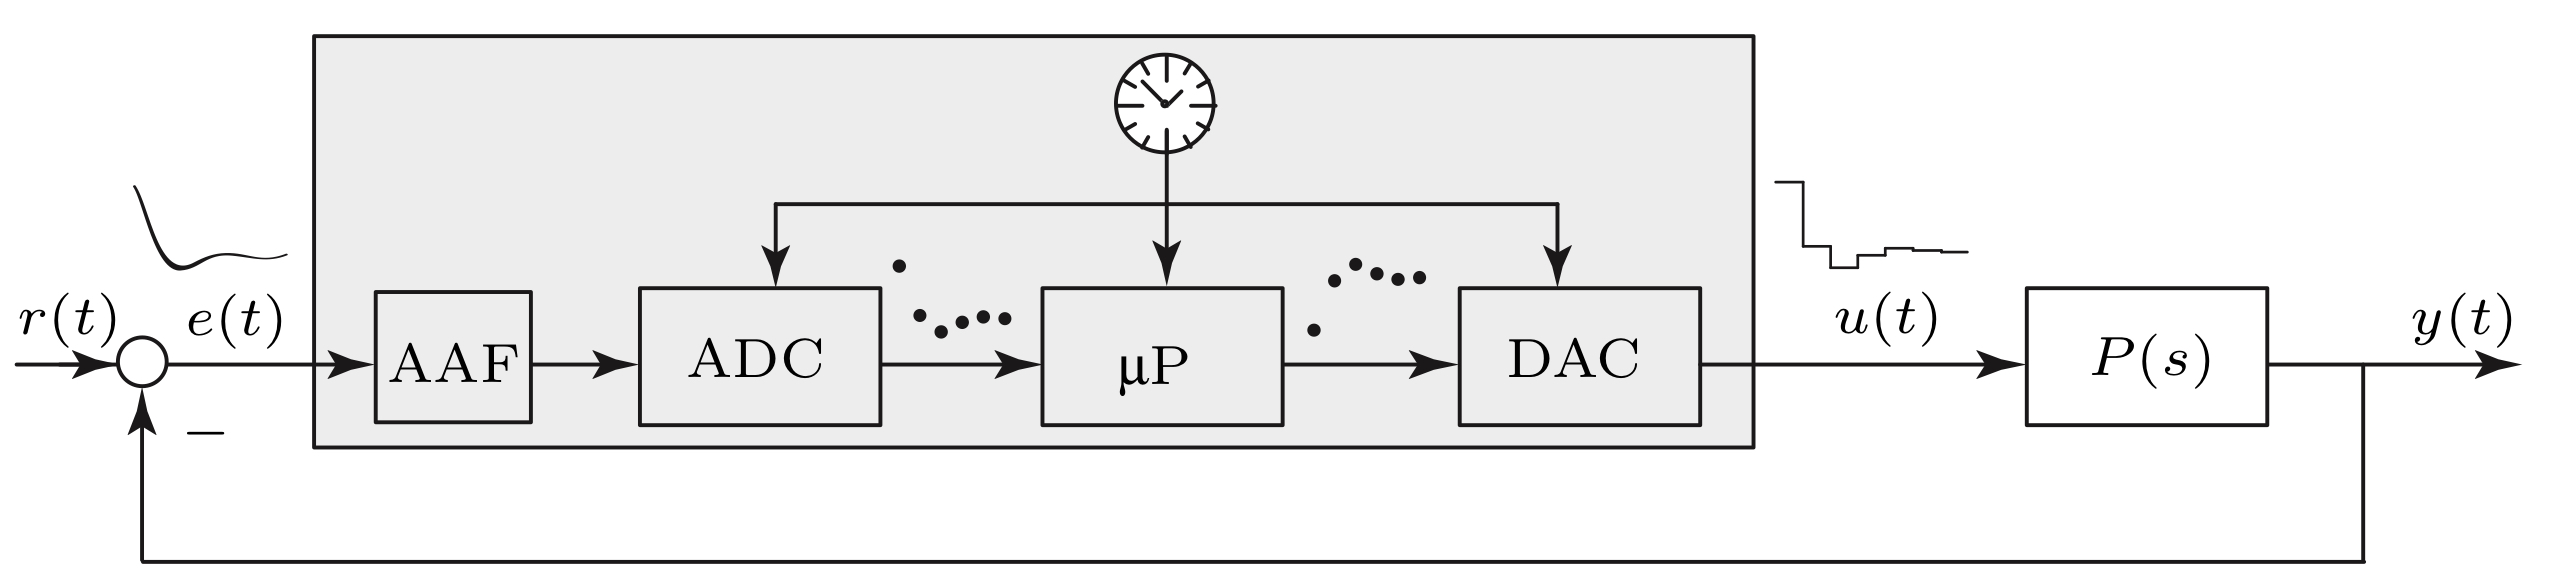
\includegraphics[width = 0.6\linewidth]{images/04/disc_time.jpeg}
        \caption{digitales Regelsystem}
    \end{figure}
    \begin{itemize}
        \item ADC: Analog-to-Digital Converter. Konvertiert zeit-kontinuierliche Signale in zeit-diskrete.
        
        \item $\mu$P: Mikroprozesser. Berechnet zeit-diskreten Eingang $u[k]$.
        
        \item DAC: Digital-to-Analog-Converter Konvertiert zeit-diskrete Signale in zeit-kontinuierliche (meistens ein \textit{Zero-order Hold}).
        \begin{equation*}
            u(t) = u[k] \quad \forall t\in [k\cdot T_s,(k+1)\cdot T_s]
        \end{equation*}
    \end{itemize}
    
    \begin{figure}[H]
        \centering
        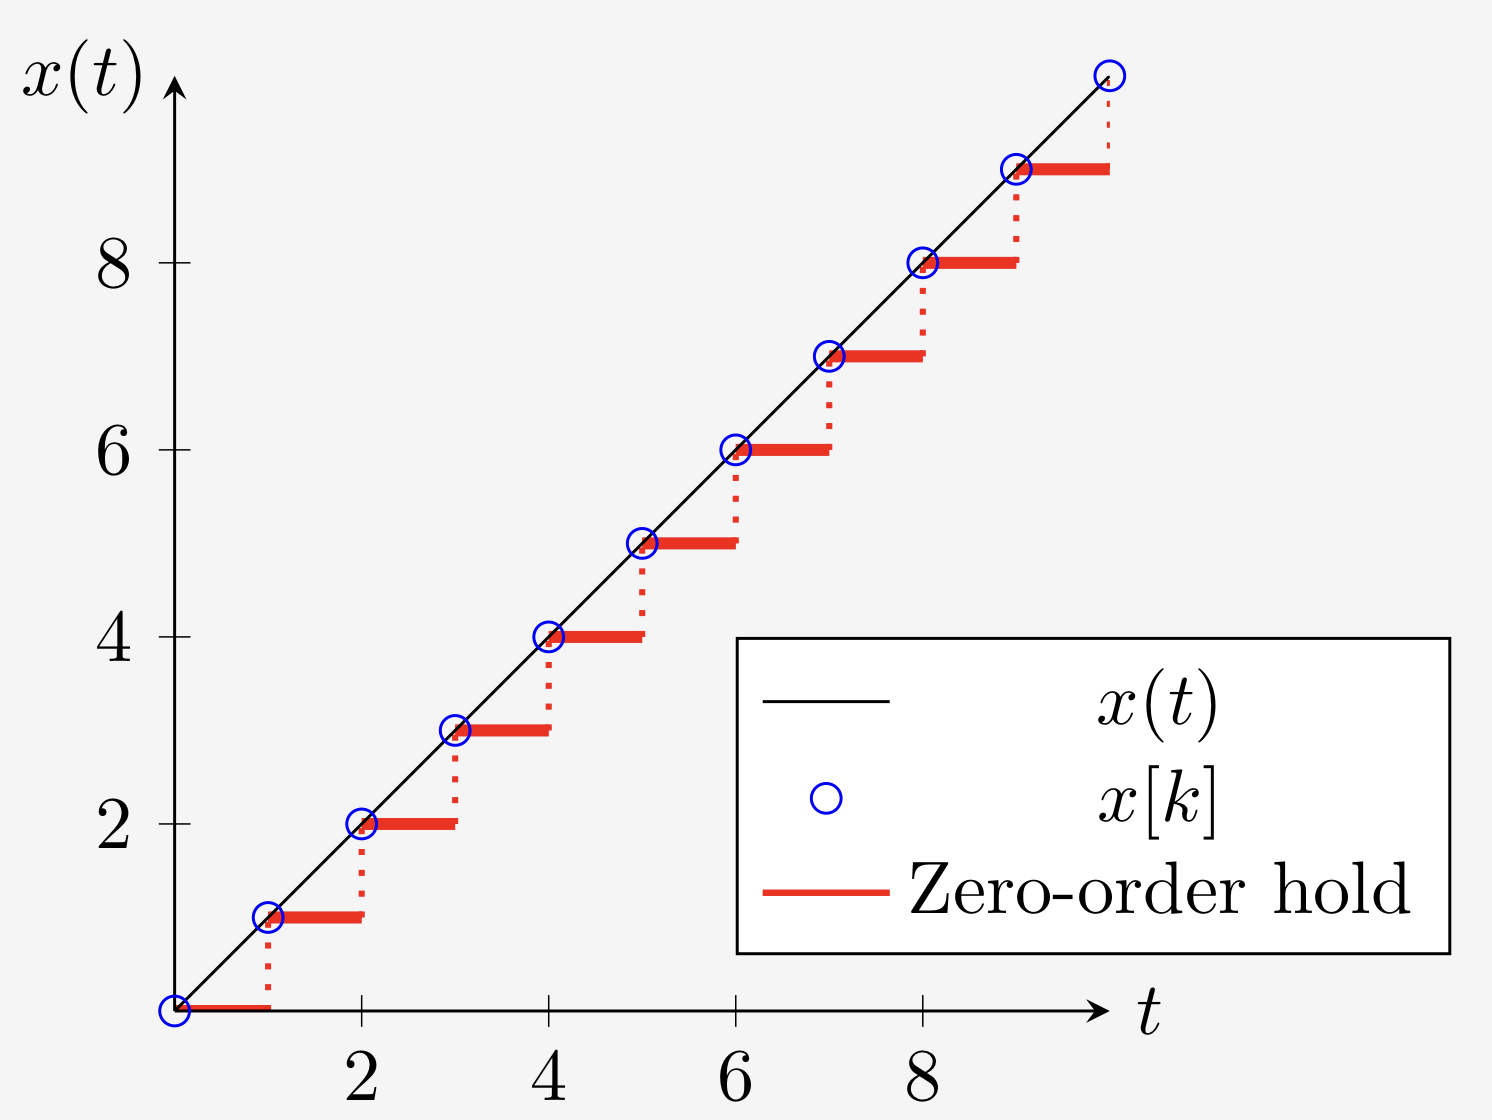
\includegraphics[width = 0.45\linewidth]{images/04/0order_hold.jpeg}
        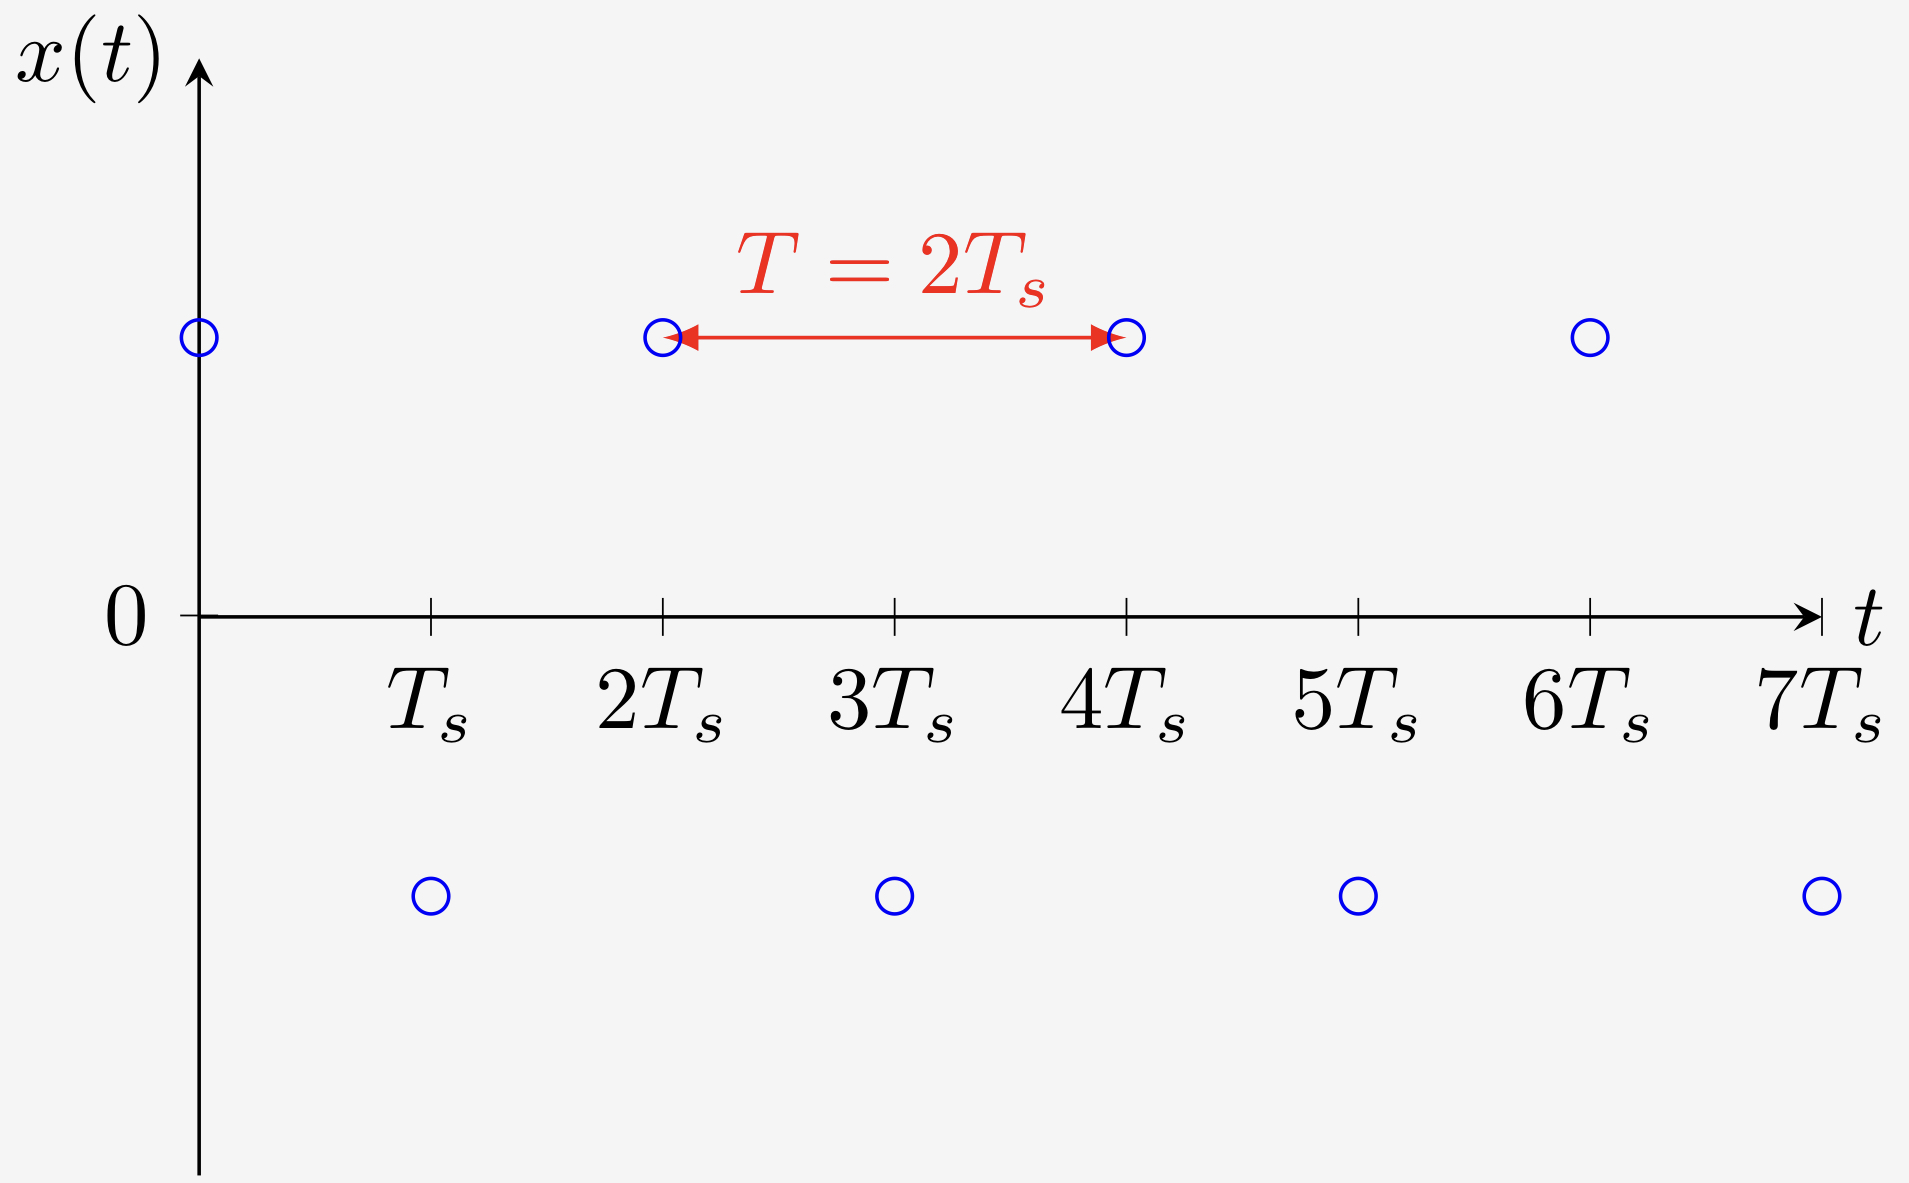
\includegraphics[width = 0.45\linewidth]{images/04/freq_disctime.jpeg}
    \end{figure}
    
    Für eine fixe Rate $\mathit{f}_s = \frac{1}{T_s}$ soll man ein Signal Zeichnen, welches die höchstmögliche Frequenz hat. Die höchstmögliche Frequenz, die man in das Zeitraster $\{0,T_s,\dots\}$ legen kann lautet:
    \begin{equation*}
        \mathit{f}_\textnormal{max} = \frac{1}{T} = \frac{1}{2T_s} \quad \textnormal{(Nyquist Frequenz)}
    \end{equation*}
    
    \subsubsection{Z-Transform}
        \begin{equation*}
            X(z) = \mathbb{Z}\{x(k)\} = \sum_{k=0}^\infty z^{-k}\cdot x(k)
        \end{equation*}
        Eigenschaften:
        \begin{gather*}
            x(k+1) = z\cdot X(z) - z\cdot x(0)\\
            x(k-1) = z^{-1}\cdot X(z)\\
            z = e^{sT_s}
        \end{gather*}
    
    \subsubsection{Emulation}
        Da $z(s)$ nichtlinear ist benutzt man approximationen um einen Regler zu emulieren. Emulationen sind dann sinnvoll, wenn die diskreten Zeitrschritte $T_s$ sehr klein sind im Vergleich zur Systemdynamik.
        \begin{align*}
            z &= e^{sT_s}    &   &\approx 1+sT_s    &   &\Rightarrow s\approx \frac{z-1}{T_s} &   &\textnormal{Euler Forward}\\
            z &= \frac{1}{e^{-sT_s}}    &   &\approx \frac{1}{1-sT_s}    &   &\Rightarrow s\approx \frac{z-1}{zT_s}  &   &\textnormal{Euler Backward}\\
            z &= \frac{e^{sT_s/2}}{e^{-sT_s/2}}    &   &\approx \frac{1+sT_s/2}{1-sT_s/2}    &   &\Rightarrow s\approx \frac{2(z-1)}{T_s(z+1)}  &   &\textnormal{Tustin Emulation}\\
        \end{align*}
        
        Die Tustin emulation ist die am häufigste verwendete emulation, insbesondere weil damit die ganze linke $s$-Halbebene in der $z$-Ebene in einen Kreis mit Radius kleiner eins ($|z|<1$) gemappt wird. D.h. ein stabiles kontinuierliches System resultiert in einem stabilen diskreten System (Stabil in $z \Leftrightarrow |z|<1$). Euler backward erfüllt diese Kriterium auch, Euler backward hingegen nicht. 
        

    
    
    
\section{Numerische Verfahren}
    Mit numerischen Verfahren kann man für fixe Regelstrukturen (z.B: PI) ein Optimierungsproblem lösen, um die Parameter $k_p,\, T_i$ zu bestimmen. Dazu stellt man eine Kostenfunktion $J(k_p,T_i)$ auf, welche man durch die Wahl der optimalen Pramater $k_p^\star$ und $T_i^\star$ minimieren will.

\textbf{Beispiele für Gütekriterien:}
\begin{itemize}
    \item kumulativer Fehler über den quadrieten Fehler:
        \begin{equation*}
            g_1 = \int_0^\infty e^2(t)dt
        \end{equation*}
    
    \item Der maximale Überchuss von $y(t)$:
        \begin{equation*}
            g_2 = \max_{t\in[0,\infty)}(y(t)-1)
        \end{equation*}
    
    \item Robustheit über Minimum return difference $\mu$\textsubscript{min}
        \begin{equation*}
            g_3 = 1 -\mu_{\textnormal{min}} = 1 - \max_{\omega\in[0,\infty)}|1 + L(\jw)|
        \end{equation*}
\end{itemize}

Die Kostenfunktion ist daher $J(k_p,T_i) = \kappa_1\cdot g_1 + \kappa_2\cdot g_2 + \kappa_3\cdot g_3$. Das resultierende Optimierungsproblem 
\begin{equation*}
    \min_{k_p,T_i}J(k_p,T_i)    
\end{equation*}
kann in MATLAB mit \texttt{fminsearch} gelöst werden, wobei $\kappa_{(\cdot)}$ ein Mass für die Wichtigkeit einer Grösse $g_{(\cdot)}$ sind. Je Grösser ein $\kappa_{(\cdot)}$ ist, desto mehr wird das dazugehörige $g_{(\cdot)}$ bestraft. Dadurch werden die anderen Kriterien, relativ zum höher gewichtetn Kriterium, weniger gewichtet.



    
\vfill\null\columnbreak
\section{Algebraishe Stabilität}
    Man möchte wissen, ob ein Polynom
\begin{equation*}
    a_n\cdot s^n + a_{n-1}\cdot s^{n-1} + \dots + a_1\cdot s + a_0,\quad a_n > 0
\end{equation*}
alle NST in der linken komplexen Halbebene hat. Bedingung $a_i>0\, \forall i$ ist notwendig aber nicht hinreichend \Big(alle  NST MMP $\underset{\not\Leftarrow}{\Rightarrow} a_i > 0$\Big).

\subsection{Hurwitz Kriterium}
    Koeffizienten $a_i$ bekannt. Falls alle Matrizen
    \begin{equation*}
        H_1 = a_{n-1}, \,
        H_2 =
        \begin{bmatrix}
            a_{n-1} & a_n\\
            a_{n-3} & a_{n-2}
        \end{bmatrix}, \,
        H_3 = 
        \begin{bmatrix}
            a_{n-1} & a_n   & 0\\
            a_{n-3} & a_{n-2} & a_{n-1}\\
            a_{n-5} & a_{n-4} & a_{n-3}
        \end{bmatrix}, \, \dots
    \end{equation*}
    positiv definit sind (alle EW grösser als 0), dann sind alls NST in der linken komplexen Halbebene.
    
\subsection{Kharitonov Kriterium}
    Die Koeffizienten $a_i$ seien nicht exakt bekannt, man weiss jedoch, dass sie in einer gewissen Region liegen:
    \begin{equation*}
        p(s,a) = [\underline{a}_n,\overline{a}_n]\cdot s^n +  [\underline{a}_{n-1},\overline{a}_{n-1}]\cdot s^{n-1} + \dots +  [\underline{a}_0,\overline{a}_0]
    \end{equation*}
    
    Das Problem reduziert sich auf die Ecken eines Rechtecks in der komplexen Ebene und es müssen nur folgende Polynome mit dem Hurwitz Kriterium getestet werden:
    \begin{align*}
        p_1(s) &= \overline{a}_0 + \underline{a}_1\cdot s +\underline{a}_2\cdot s^2 + \overline{a}_3\cdot s^3 + \dots\\
        p_2(s) &= \overline{a}_0 + \overline{a}_1\cdot s +\underline{a}_2\cdot s^2 + \underline{a}_3\cdot s^3 + \dots\\
        p_3(s) &= \underline{a}_0 + \overline{a}_1\cdot s +\overline{a}_2\cdot s^2 + \underline{a}_3\cdot s^3 + \dots\\
        p_3(s) &= \underline{a}_0 + \underline{a}_1\cdot s +\overline{a}_2\cdot s^2 + \overline{a}_3\cdot s^3 + \dots\\
    \end{align*}
    \subsection{Bsp}
    Wir wollen $k_{p,\textnormal{max}}$ bestimmen, für welches folgende Strecke noch stabil bleibt.
    \begin{equation*}
        P(s) = -42\frac{(2-6.8)(s+6.8)}{s(s+5.8)(s^2+22.2s+126.9)}
    \end{equation*}
    Mithilfe Nyquist-Stabilitätskriterium:
    \begin{itemize}
        \item $\hat{\omega}$ bestimmen, wo $\operatorname{Im}\big(P(j\hat{\omega})\big)=0$      wird.
            \begin{align*}
                P(\jw)  &= \frac{42\omega^2+1946}{\omega^4-j\cdot28\omega^3-255\omega^2+j\cdot731\omega}\\
                &= \frac{42\omega^2+1946}{\omega^4-255\omega^2+j\cdot(731\omega-28\omega^3)}\\
                &\Rightarrow 731\hat{\omega}-28\hat{\omega}^3 \overset{!}{=} 0 \Rightarrow \hat{\omega} = \sqrt{\frac{731}{28}}
            \end{align*}
        
        \item $|P(j\hat{\omega})|$ bestimmen.
            \begin{equation*}
                |P(j\hat{\omega})| = \left|\frac{42\hat{\omega}^2 + 1946}{\hat{\omega}^4-255\hat{\omega}^2}\right| \approx 0.51
            \end{equation*}
        
        \item $k_{p,\textnormal{max}}$ bestimmen.
            \begin{equation*}
                k_{p,\textnormal{max}} = \frac{1}{0.51} = 1.96
            \end{equation*}
    \end{itemize}
    Anhand Hurwitz-Kriterium:
    \begin{itemize}
        \item $T(s)$ als Funktion von $k_p$ bestimmen.
            \begin{align*}
                P(s) &= \frac{a(s)}{b(s)},\quad C(s) = k_p\\
                L(s) &=  k_p\frac{a(s)}{b(s)}\\
                T(s) &=  \frac{k_p\cdot a(s)}{b(s) + k_p\cdot a(s)}
            \end{align*}
            Für die Stabilität interessirt und also ob $b(s) + k_p\cdot a(s)$ alle NST in der linken Halbebene hat.
            \begin{equation*}
                b(s) + k_p\cdot a(s) = s^4 + 28s^3 + (255-42k_p)s^2 + 731s + 1946k_p
            \end{equation*}
        
        \item Nun prüfen wir das Hurwitz-Kriterium:
            \begin{align*}
                H_4 &= 
                \begin{bmatrix}
                a_{n-1} & a_n & 0 & 0\\
                a_{n-3} & a_{n-2} & a_{n-1} & a_n\\
                a_{n-5} & a_{n-4} & a_{n-3} & a_{n-2}\\
                a_{n-7} & a_{n-6} & a_{n-5} & a_{n-4}
                \end{bmatrix}\\
                &= 
                \begin{bmatrix}
                28 & 1 & 0 & 0\\
                731 & 255-42k_p & 28 & 1\\
                1946k_p &731 & 255-42k_p & 28\\
                0   &   0   &   0   &   1946k_p
                \end{bmatrix}
            \end{align*}
            Für die führenden Hauptminoren muss gelten: $d_i > 0$
            \begin{gather*}
                d_1 = 28 > 0,\quad  d_2 = (6409-1176k_p) > 0 \Rightarrow k_p < 5.45\\
                d_3 = 4684979-2385320k_p \Rightarrow k_p < 1.96,\quad d_4 = d_3\cdot1946k_p 
            \end{gather*}
            Somit muss für Stabilität gelten: $k_p\in(0,\,1.96)$
    \end{itemize}

\vfill\null\columnbreak 
\section{MIMO}
    \subsection{Systembeschreibung}
    MIMO systeme haben mehrere Ein- und Ausgänge, d.h. $u(t) \in \mathbb{R}^m$, $y(t) \in \mathbb{R}^p$ und $x(t) \in \mathbb{R}^n$ dementsprechend sind Matrizen $B,\ C,\ D$ auf die Dimensionen angepasst werden.
    dabei gilt für das I/O verhalten die selbe Herleitung, wie bei einem SISO System
    \[s\cdot X(s) = A \cdot X(s) + B\cdot U(s)\]
    \[\Rightarrow X(s) = (s\cdot I_{n\times n} - A) ^{-1}\cdot B \cdot U(s)\]
    \[\Rightarrow Y(s) = \underbrace{(C\cdot(s\cdot I_{n\times n} -A)^{-1}\cdot B+D)}_{\text{P(s)}}\cdot U(s)\]
    da $U(s)\in \mathbb{C}^m$ und $Y(s)\in \mathbb{C}^p$ wird $P(s)$ eine Matrix: 
    \[P(s) = \begin{bmatrix}
    P_{1,1}(s) & P_{1,2}(s) & \hdots & P_{1,m}(s) \\
    P_{2,1}(s) & P_{2,2}(s) & \hdots & P_{2,m}(s) \\
    \vdots & \vdots & \ddots & \vdots \\
    P_{p,1}(s) & P_{p,2}(s) & \hdots & P_{p,m}(s)
    \end{bmatrix}\]
    Wobei jede Übertragungsfunktion $P_{i,j}(s):\ u_j \rightarrow y_i$
    \[P_{i,j}(s) = \frac{b_{m,i,j}s^m+\dots + b_{1,i,j}s+ b_{0,i,j}}{s^n + a_{n-1,i.j}s^{n-1}+\dots + a_{1,i,j}s + a_{0,i,j}} = \frac{b_{i,j}(s)}{a_{i,j}(s)}\]
    eine gebrochenrationale Funktion darstellt. 
    Note: $P(s)$ beinhaltet nur steurbare und beobachtbare Teile des Systems.
    
\subsection{Sensitivitäten}
    Wie auch im SISO Fall können wir die Sensitivitäten für ein MIMO System beschreiben:
    \begin{equation*}
    \colorboxed{red}{
    \begin{aligned}
        L(s) &= \frac{Y(s)}{E(s)} = P(s)\cdot C(s)\\
        S(s) &= \frac{E(s)}{R(s)} =\big(I + L(s)\big)^{-1}\\
        T(s) &= \frac{Y(s)}{R(s)} = L(s)\cdot \big(I + L(s)\big)^{-1}
    \end{aligned}
    }
    \end{equation*}
    Es gilt die Identität: $G_1\big(I-G_2G_1\big)^{-1} = \big(I - G_1G_2\big)^{-1}G_1$
    
\subsection{Stabilität, Steuerbarkeit und Beobachtbarkeit}
    Die Analyse von MIMO Systemen ist identisch zu derjenigen von SISO Systemen. 
    \subsubsection{Stabilität nach Lyapunov}
    \textbf{asymptotisch stabil} nach Lyapunov: 
    Alle Eigenwerte von A haben negativen Realteil, $Re(\lambda_i) < 0$
    
    \textbf{stabil} nach Lyapunov:
    Mindestens ein Eigenwert $\lambda_k$ von $A$ hat Realteil $Re(\lambda_k) = 0$ und alle anderen Eigenwerte haben negative Realteile.
    
    \textbf{instabil}nach Lyapunov:
    Mindestens ein Eigenwert $\lambda_k$ von $A$ hat einen positiven Realteil $Re(\lambda_k) > 0$
    
    \subsubsection{Steuerbarkeit}
        Das System $\{A,\ B,\ C,\ D\}$ ist vollständig steuerbar, falls die Steuerbarkeitsmatrix $\mathcal{R}_n$ vollen Rang $n$ hat
    \[\mathcal{R}_n = [B,\ AB,\ \dots,\ A^{n-1}B]\in \mathbb{R}^{n\times(n\cdot m)}\]
    
    \subsubsection{Beobachtbarkeit}
        Das System $\{A,\ B,\ C,\ D\}$ ist vollständig steuerbar, falls die Beobachtbarkeitsmatrix $\mathcal{O}_n$ vollen Rang $n$ hat
        \[\mathcal{O}_n = \begin{bmatrix} C\\ CA\\ \vdots\\ CA^{n-1}\end{bmatrix}\in \mathbb{R}^{(n\cdot p)\times n}\]
    \subsubsection{System Minimalisierung}
        Zustandsraummodell ist nur dann eine Minimalerealisierung, wenn es vollständig Steuerbar und Beobachtbar ist.
        Minimale Systemordnung := \#Pole, Pole kann man bei MIMO-Systemen nur mit Nullstellen kürzen falls auf den selben Input-Output-Pfad wirken.
        
        
    \subsection{Pole und Nullstellen} 
    % Pole und Nullstellen sind im MIMO Fall etwas komplizierter.
\subsubsection{Definition Matrix Minoren}
        Minoren einer Matrix sind die Determinanten aller quadratischen Submatrizen. Die Submatrizen werden durch Streichen einzelner Zeilen und Spalten der Matrix gebildet.

    \subsubsection{Polstellen von MIMO Systemen}
        Die Pole von$P(s)$ sind die Nullstellen des kleinsten gemeinsamen Vielfachen (kgV) der Nennerpolynome aller Minoren von $P(S)$

    \subsubsection{Nullstellen von MIMO Systemen}
        Die Nullstellen von $P(s)$ sind die Nullstelle des grössten gemeinsamen Teilers (ggT) der Zähler der Minoren höchster Ordnung von $P(s)$ nach der Normalisierung, bei der alle Pole von $P(s)$ im Nenner stehen.
        
        Note: Nullstellen $s=\zeta_i$ sind nicht triviale Frequenzen, bei denen für ein spezifisches Eingangssignal $u(t)$ und spezifische Anfangsbedingungen $x(0)$ gilt: $y(t) = 0 \,\forall t$

        D.h. die folgende Laplace Transformation erfüllt
        \begin{align*}
            (sI_{n\times n} -A)\cdot x - B \cdot u &= 0\\
            C\cdot x + D \cdot u &= 0
        \end{align*}
        wobei nur eine nichttriviale Lösung besteht, falls die folgende Matrix singulär ist: 
        \begin{equation*}
            \det\begin{bmatrix}
                (sI_{n\times n}- A) & -B \\
                C& D
            \end{bmatrix} = 0
        \end{equation*}


        \subsubsection{Bsp}
        Wir wollen ein MIMO System mit einen P-Regler regeln. Dabei vernachlässigen wir die Kreuzkopplungen und gehen davon aus, dass $u_1 \rightarrow y_1$ und $u_2 \rightarrow y_2$ regelt.
        \begin{equation*}
            P(s) =
            \begin{bmatrix}
            \frac{2}{s+1}  &    \frac{3}{s+2}\\
            \frac{1}{s+1}  &    \frac{1}{s+1}
            \end{bmatrix}
            \qquad
            C(s) = 
            \begin{bmatrix}
            K_1 & 0\\
            0   & K_2
            \end{bmatrix}
        \end{equation*}
        \textit{Q: Wie gross können wir $K_i$ wählen, ohne die Stabilität zu gefährden?}
        
        A: 
        \begin{gather*}
            T_1(s) = \frac{K_1\frac{2}{s+1}}{1 + K_1\frac{2}{s+1}} = \frac{2K_1}{s +(2K_1 + 1)},\\
            T_2(s) = \frac{K_2\frac{1}{s+1}}{1 + K_2\frac{1}{s+1}} = \frac{K_2}{s + (K_2 + 1)}\\
            \Rightarrow 2K_1 + 1 > 0, \qquad K_2 + 1 > 0\\
            \Rightarrow K_1 > -\frac{1}{2},\, K_2 > -1,\, \textnormal{bzw:}\, K_i > 0
        \end{gather*}
        
    \subsubsection{Bsp}
        Bestimme die Pol- und Nullstellen von
        \begin{equation*}
            P(s) = 
            \begin{bmatrix}
            \frac{1}{s+1}   &   0   &   \frac{s-1}{(s+1)(s+2)}\\
            \frac{-1}{s-1}  &   \frac{1}{s+2} & \frac{1}{s+2}
            \end{bmatrix}
        \end{equation*}
        bestimmen.
        
        Für die Pole bestimmen wir zuerst die Minoren:
        \begin{gather*}
            \frac{1}{s+1},\qquad 0,\qquad \frac{s-1}{(s+1)(s+2)}\\
            \frac{-1}{s-1},\qquad \frac{1}{s+2},\qquad \frac{1}{s+2}\\
            \frac{1}{(s+1)(s+2)},\qquad \frac{2}{(s+1)(s+2)},\qquad \frac{(-1)(s-1)}{(s+1)(s+2)^2}
        \end{gather*}
        KGV\textsubscript{Nenner} ist daher:
        \begin{gather*}
            (s+1)(s+2)^2(s-1)\\
            \pi_1 = -1,\quad \pi_{2,3} = -2,\quad \pi_4 = 1
        \end{gather*}
        
        Um die (Übertragungs-)Nullstellen des Systems zu bestimmen erweitern wir die Minoren höchster Ordnung (Von den ``grössten" Determinanten):
        \begin{equation*}
            \frac{\textcolor{red}{(s+2)(s-1)}}{(s+1)(s+2)\textcolor{red}{^2(s-1)}},\quad \frac{2\textcolor{red}{(s+2)(s-1)}}{(s+1)(s+2)\textcolor{red}{^2(s-1)}},\quad \frac{(-1)(s-1)\textcolor{red}{^2}}{(s+1)(s+2)^2\textcolor{red}{(s-1)}}
        \end{equation*}
        
        GGT\textsubscript{Zähler} ist somit:
        \begin{equation*}
            (s-1) \Rightarrow \zeta_1 = 1
        \end{equation*}
        
        \textit{Q: Was ist die minimale Ordnung einer internen Beschreibung?}
        
        A: Es wurden 4 Pole gefunden, somit besitzt eine interne Beschreibung des Systems mindestens 4. Ordnung. \textbf{Bemerkung:} Ein Mehrgrössensystem kann Pole und NST bei den gleichen Frequenzen haben, ohne dass sich diese kürzen, da es darauf ankommt, ob die dieselbe Frequenz \textit{und} Richtung haben.
        

\vfill\null\columnbreak 
\section{RGA}
    RGA wird benutzt, um systematisch zu überprüfen, wie SISO ähnlich ein System ist. Das Ziel ist es zu bestimmen ob ein $m \times m$ MIMO-system auch mit einem $m$ SISO-Kontroller eine befriedigende Kreisverstärkung erzielen kann. 
Das RGA ist schlussendlich eine Matrix mit den Verhältnissen aller Übertragungsfunktionen bei einer gegebenen Frequenz $\omega$ 

Die Extremfälle für die Übertragungsfunktion $P_{11}$ werden illustrativ mit folgender Abbildung dargestellt: 
\begin{center}
    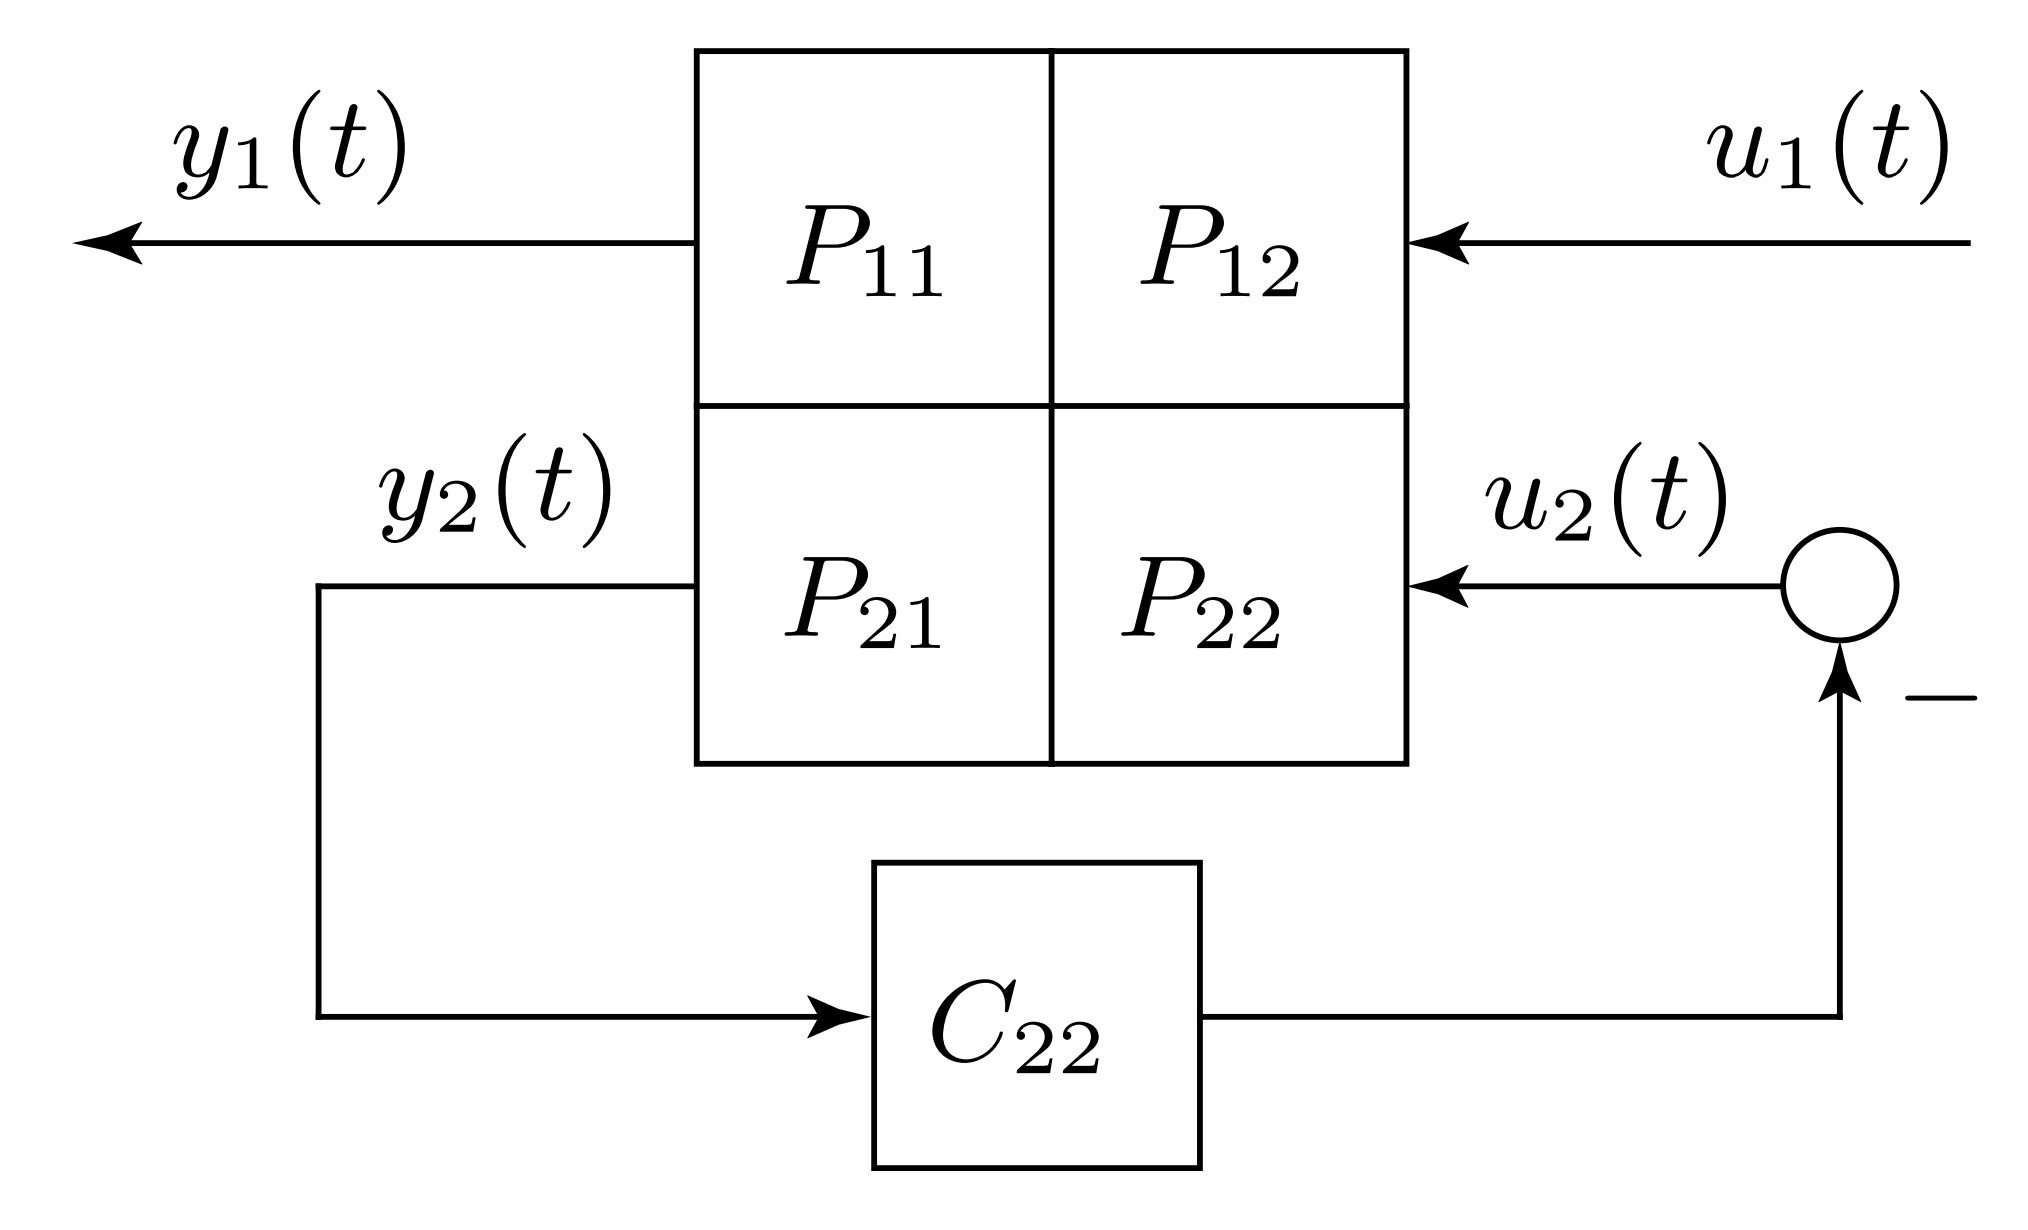
\includegraphics[width = 0.4\linewidth]{images/06/RGA.jpg}
\end{center}
Der Regler $C_{22}$ sollte dabei als eine Art hypothetische Grösse verstanden werden, mit der entweder $u_{2}(t) = 0$ oder $y_2(t)=0$ gesetzt werden kann.

\textbf{Extremfall 1: 'open-loop'} $\boxed{C_{22} = 0}$

Das System wird 'open-loop' betrachtet: Es wird angenommen dass der Regler $C_{22} = 0$ ist, d.h dass nur der Eingang $u_1$ den Ausgang $y_1$ beeinflusst. während im allgemeinen Fall alle anderen Eingänge null sind: $u_j=0 \forall j \setminus \{1\}$
in diesem Fall ist die Übertragungsfunktion von $u_1$ auf $y_1$: 
\[P_{u_1\rightarrow y_1}(s) = P_{11}(s)\]
\textbf{Extremfall 2: 'perfect closed-loop'} $\boxed{C_{22}= \infty}$

Es wird angenommen, dass im allgemeinen Fall alle Ausgänge ausser der betrachtete Ausgang $y_1$ perfekt auf null geregelt werden, d.h. $y_i = 0 \forall i \setminus \{1\}$. Im gegebenen Beispiel heisst das, dass $u_2(t)$ so gewählt ist, dass $y_2(t) = 0 \forall t$. Dies wird schematisch mit einem Regler unendlicher Verstärkung $C_{22} = \infty$ dargestellt. Dann ist die Übertragungsfunktion von $u_1$ auf $y_1$:
\[P_{u_1 \rightarrow y_1}(s) = \frac{P_{11}(s)\cdot P_{22}(s) - P_{12}(s)\cdot P_{21}(s)}{P_{22}}\]
\textbf{Der Relative Gain} ist das resultierende Verhältnis zwischen open-loop und closed-loop Verhalten:\[[\,RGA(s)]\,_{11} = \frac{P_{11}(s)\cdot P_{22}(s)}{P_{11}(s)\cdot P_{22}-P_{12}(s)\cdot P_{21}(s)}\]

Dieses Verhältnis hat eine sehr schöne Interpretation: Es wiederspiegelt die änderung der Verstärkung von Eingang $u_1$ auf Ausgang $y_1$ im Fall , dass alle anderen Regelkreise des MIMO Systems perfekt geschlossen werden. Der Relative Gain beantwortet also die Frage: \textit{Wenn ein Regler vom Eingang $u_1$ auf den Ausgang $y_1$ basierend auf dem open-loop System $P_{11}$ ausgelegt wird, welche veränderten Verhältnisse trifft dieser Regler an, wenn er schlussendlich im geregelten MIMO-System verwendet wird?}

\textbf{SISO-fähiges $P_{i,j}(s)$} $\boxed{[\,RGA(s)]\,_{ij}\approx 1}$  

Die Verstärkung von Eingang $u_j$ auf den Ausgang $y_i$ im MIMO-Sysgem ist identischzu Verstärkung der Übertragungsfunktion $P_{ij}(s)$Basierend auf $P_{ij}(s)$ kann also ein sinnvoller Regler entworfen werden, der den Ausgang $y_i$ mit dem Eingang $u_j$ regelt.

\textbf{Nicht SISO-fähiges $P_{ij}(s)$}$\boxed{[\,RGA(s)]\,_{ij}\approx 0}$  
Die Verstärkung der Übertragungsfunktion $P_{ij}(s)$ ist vernachlässigbar im Vergleich zur resultierenden Verstärkung von Eingang $u_j$ auf Ausgang $y_i$ im MIMO System. Basierend auf $P_{ij}(s)$ kann also \underline{kein} sinnvoller Regler werden der den Ausgang $y_i$ mit dem Eingajng $u_j$ regelt.

\textbf{Instabiles Verhalten für $P_{ij}(s)$} $\boxed{[\,RGA(s)]\,_{ij}<0}$
Das Vorzeichen der Verstärkung der Übertragungsfunktion von $u_j$ auf $y_i$ im MIMO System ist unterschiedlich vom Vorzeichen von $P_{ij}(s)$. D.h. ein SISO-Regler, ausgelegt basierend auf $P_{ij}(s)$, hat wenn er im MIMO-System verwendet wurd, eine entgegengesetzte Wirkung. Der Regler führt also z.B als Reaktion auf einen Sollsprung in $y_i$ dazu, dass die Variable $y_i$ nach unten anstatt nach oben gereglet wird, das MIMO System kann mit diesem Regler also destabilisert werden. 

\textbf{Das RGA} ist die Matrix mit den relativen gains aller Übertragungsfunktionen als Einträgen. 

Das RGA einer $2 \times 2$ Regelstrecke $P(s)$ ist: 
\begin{equation*}
\colorboxed{red}{
RGA(s) = 
{\renewcommand{\arraystretch}{2}
\begin{bmatrix}
\frac{P_{11}P_{22}}{P_{11}P_{22}-P_{12}P_{21}} & \frac{-P_{12}P_{21}}{P_{22}P_{11}-P_{21}P_{12}}\\
\frac{-P_{12}P_{21}}{P_{22}P_{11}-P_{21}P_{12}} & \frac{P_{11}P_{22}}{P_{11}P_{22}-P_{12}P_{21}}
\end{bmatrix}
}
}
\end{equation*}

das RGA eines allgemeinen MIMO-Systems $P(s)$ kann wie folgt berechnet werden: 
\[
\colorboxed{red}{
RGA(s) = P(s).\times P(s)^{-\top}
}
\] wobei $.\times$ eine elementweise Multiplikation beschreibt und $P(s)^{-T}$ die Inverse der Transponierten ist. 

\textbf{Eigenschaften des RGA:} 
\begin{itemize}
    \item Die Summe der Spalten und der Zeilen des RGA ergeben immer 1.
    
    \item Ist das RGA bei einer gegebenen Frequenz $\omega$ ungefähr eine Einheitsmatrix:
    \begin{equation*}
        \big[RGA(\jw)\big]\approx 
        {\renewcommand{\arraystretch}{1.5}
        \begin{bmatrix}
            1&0&0\\
            0&\ddots&0\\
            0&0&1
        \end{bmatrix}
        },
    \end{equation*}
    dann ist das betrachtete MIMO-System bei dieser Frequenz mit individuellen SISO-Reglern regelbar.
\end{itemize}
\textbf{Allgemein:} falls in jeder Zeile/Spalte ein Eintrag sehr nahe bei 1 ist und die anderen nahe bei 0, sind diese Kombinationen von Ein- und Ausgängen gut mit einem SISO-Regler regelbar.



\vfill\null\columnbreak 
\section{Singulärwerte}
    \subsection{Singulärwerte}
    Im folgenden werden Eigenschaften zur linearen Abbildung\[y= M \cdot u,\ u \in \mathbb{C}^m,\ y\in\mathbb{C}^p,\ M\in\mathbb{C}^{p\times m}\]
    beschrieben. Insbesondere erfüllt der Ausgang $y$ folgende wichtige Eigenschaft:\[\sigma_{\textnormal{min}}(M)\leq\frac{||y||}{||u||}\leq\sigma_{\textnormal{max}}(M),\]
    wobei $||.||$ die euklische Norm ist und 
    \[\sigma_i(M)=\sqrt{\lambda_i(\overline{M}^T\cdot M)}>0,\]

    Die Singulärwerte der Matrix $M$ sind.

    $\overline{M}^T$ sit die Transponierte der komplex-Konjugierten von M. Die Singulärwertzerlegung (SVD) der Matrix $M$ lautet:
    \[M = U\cdot\Sigma V^T,\]
    Wobei $\Sigma$ die \textbf{Singulärwerte $\sigma_i$ auf der Hauptdiagonale} hat.
    $U$ und $V^T$ sind unitäre (längenerhaltende) Transformationsmatrizen:
    \[U\cdot U^T = V\cdot V^T = I\]
    \subsubsection{Vorgehen:}
        \begin{enumerate}
            \item \textbf{Singulärwerte bestimmen:}
                \[\sigma_i =\sqrt{\lambda_i(M^TM)}=\sqrt{\lambda_i(MM^T)}\]
            \item \textbf{$\Sigma \in                    \mathbb{R}^{P\times m}$ konstruieren}
                \[\Sigma = \left[\begin{array}{c c c | c}
                \sigma_1 & 0 & \dots  & 0 \\
                0&\ddots & 0 & \vdots \\
                \vdots & 0 & \sigma_r & 0 \\ \hline
                0 & \dots & 0 & 0              \end{array}\right]\ \sigma_1 \geq \sigma_2 \geq \dots \geq \sigma_r \geq 0 \] 
            \item $v_i$: Normalisierte Eigenvektoren     von $M^TM \Rightarrow$                   input-Richtungen
            \item $u_i$: Normalisierete Eigenvektoren von $MM^T
                \Rightarrow $ output-Richtungen
        \end{enumerate}
note: Falls $\sigma_i \neq 0$ geht auch: $u_i = \frac{1}{\sigma_i}Mv_i$

  
\vfill\null\columnbreak  
\section{Frequenzantworten}
    \subsection{SISO - Recap}
    Ein lineares, asymptotisch stabiles System $P(s)$, welches mit einem harmonischen Eingang
    \begin{equation*}
        u(t) = \cos\left(\omega t\right) \cdot h(t)
    \end{equation*}
    bei einer fixen Frequenz $\omega$ angeregt wird, produziert im eingeschwungenen Zustand ein harmonisches Signal bei derselben Frequenz:
    \begin{equation*}
        y_\infty(t) = |P(\jw)|\cdot\cos\left(\omega t + \angle P(\jw)\right)
    \end{equation*}
    Dabei ist die Systemantwort um $\varphi(\omega) = \angle P(\jw)$ phasenverschoben und um $ m(\omega) = |P(\jw)|$ skaliert. Um die Frequenzantwort übersichtlich darzustellen, können $|P(\jw)|$ und $\angle P(\jw)$ im Nyquist- oder Bode-Plot dargestellt werden.
    \subsection{Frequenzantwort MIMO}
    Im MIMO Fall ist der Eingang $u(t)$ ein Vektor harmonischer Funktionen:
    \begin{equation*}
        u(t)=
        \begin{bmatrix}
        \mu_1\cdot\cos\left(\omega t + \varphi_1\right)\cdot h(t)\\
        \mu_2\cdot\cos\left(\omega t + \varphi_2\right)\cdot h(t)\\
        \dots\\
        \mu_m\cdot\cos\left(\omega t + \varphi_m\right)\cdot h(t)\\
        \end{bmatrix}
    \end{equation*}
    DieFrequenzanalyse beschränkt sich auf eine gemeinsame frei wählbare Anregungsfrequenz $\omega$ auf allen Kanälen. Die Anregungsmagnituden $\mu_i$ und -phasen $\varphi_i$ können separat gewählt werden. Laplace-Transformation von $u(t)$ führt zu:
    \begin{equation*}
        U(s)=
        \begin{bmatrix}
        e^{\varphi_1\cdot s/\omega} \cdot \mu_1 \cdot \frac{s}{s^2+\omega^2}\\
        e^{\varphi_2\cdot s/\omega} \cdot \mu_2 \cdot \frac{s}{s^2+\omega^2}\\
        \dots\\
        e^{\varphi_m\cdot s/\omega} \cdot \mu_m \cdot \frac{s}{s^2+\omega^2}\\
        \end{bmatrix}
        = e^{\Phi\cdot s/\omega}\cdot \mu\cdot\frac{s}{s^2+\omega^2}
    \end{equation*}
    mit $\Phi = \operatorname{diag}(\varphi_i)\in\mathbb{R}^{m\times m}$ und $\mu = [\mu_1,\dots,\mu_m]^\top \in\mathbb{R}^m$
    
    Damit ergibt sich für den Ausgang im eingeschwungenen Zustand:
    \begin{gather*}
        y_\infty(t) = 
        \begin{bmatrix}
            \nu_1\cdot\cos\left(\omega t +\psi_1\right)\\
            \nu_2\cdot\cos\left(\omega t +\psi_2\right)\\
            \dots\\
            \nu_m\cdot\cos\left(\omega t +\psi_m\right)
        \end{bmatrix}\\
        Y(s) = e^{\Psi\cdot s/\omega}\cdot\nu\cdot\frac{s}{s^2+\omega^2}
    \end{gather*}
     mit $\Psi = \operatorname{diag}(\psi_i)\in\mathbb{R}^{m\times m}$ und $\nu = [\nu_1,\dots,\nu_m]^\top \in\mathbb{R}^m$
     
     Da für $Y(\jw) = P(\jw)\cdot U(\jw)$ gilt ergibt sich:
     \begin{gather*}
        e^{\Psi}\cdot\nu = P(\jw) \cdot e^{\Phi}\cdot \mu\\
        \underbrace{y}_{e^{\Psi}\cdot\nu} = \underbrace{M}_{P(\jw)} \cdot \underbrace{u}_{e^{\Phi}\cdot \mu}
     \end{gather*}
     Wir stellen fest, dass der Ausgang $y$ eine lineare Abbildung von $u$ ist. Es gilt daher:
     \begin{equation*}
        \sigma_\textnormal{min}\big(P(\jw)\big) \leq \frac{\|\nu\|}{\|\mu\|} \leq \sigma_\textnormal{max}\big(P(\jw)\big)
     \end{equation*}
     Die Singulärwerte geben für den eingeschwungenen Zustand Schranken für den Betrag der Amplituden $\|\nu\|$. Sie sind ein Mass für den worst-case Amplitue die man bei der Anregung einer gegebenen Frequenz $\omega$ erwarten kann.
    
    \subsubsection{Bsp}
        Wir wollen das System
        \begin{equation*}
            P(s) = 
            \begin{bmatrix}
                \frac{1}{s^2+0.3s+1} &  \frac{0.2}{s^2+0.5s+1}\\
                \frac{0.2}{s^2+s+1} &   \frac{1}{s^2+s+1}
            \end{bmatrix}
        \end{equation*}
        für $\{\mu \,|\, \|\mu\|=1\}$ bei $\omega = 0.7$ rad/s so anregen, dass $\|\nu\| = \sigma_\textnormal{max}\big(P(j\cdot0.7)\big)$ gilt.
        
        \begin{figure}[H]
            \centering
            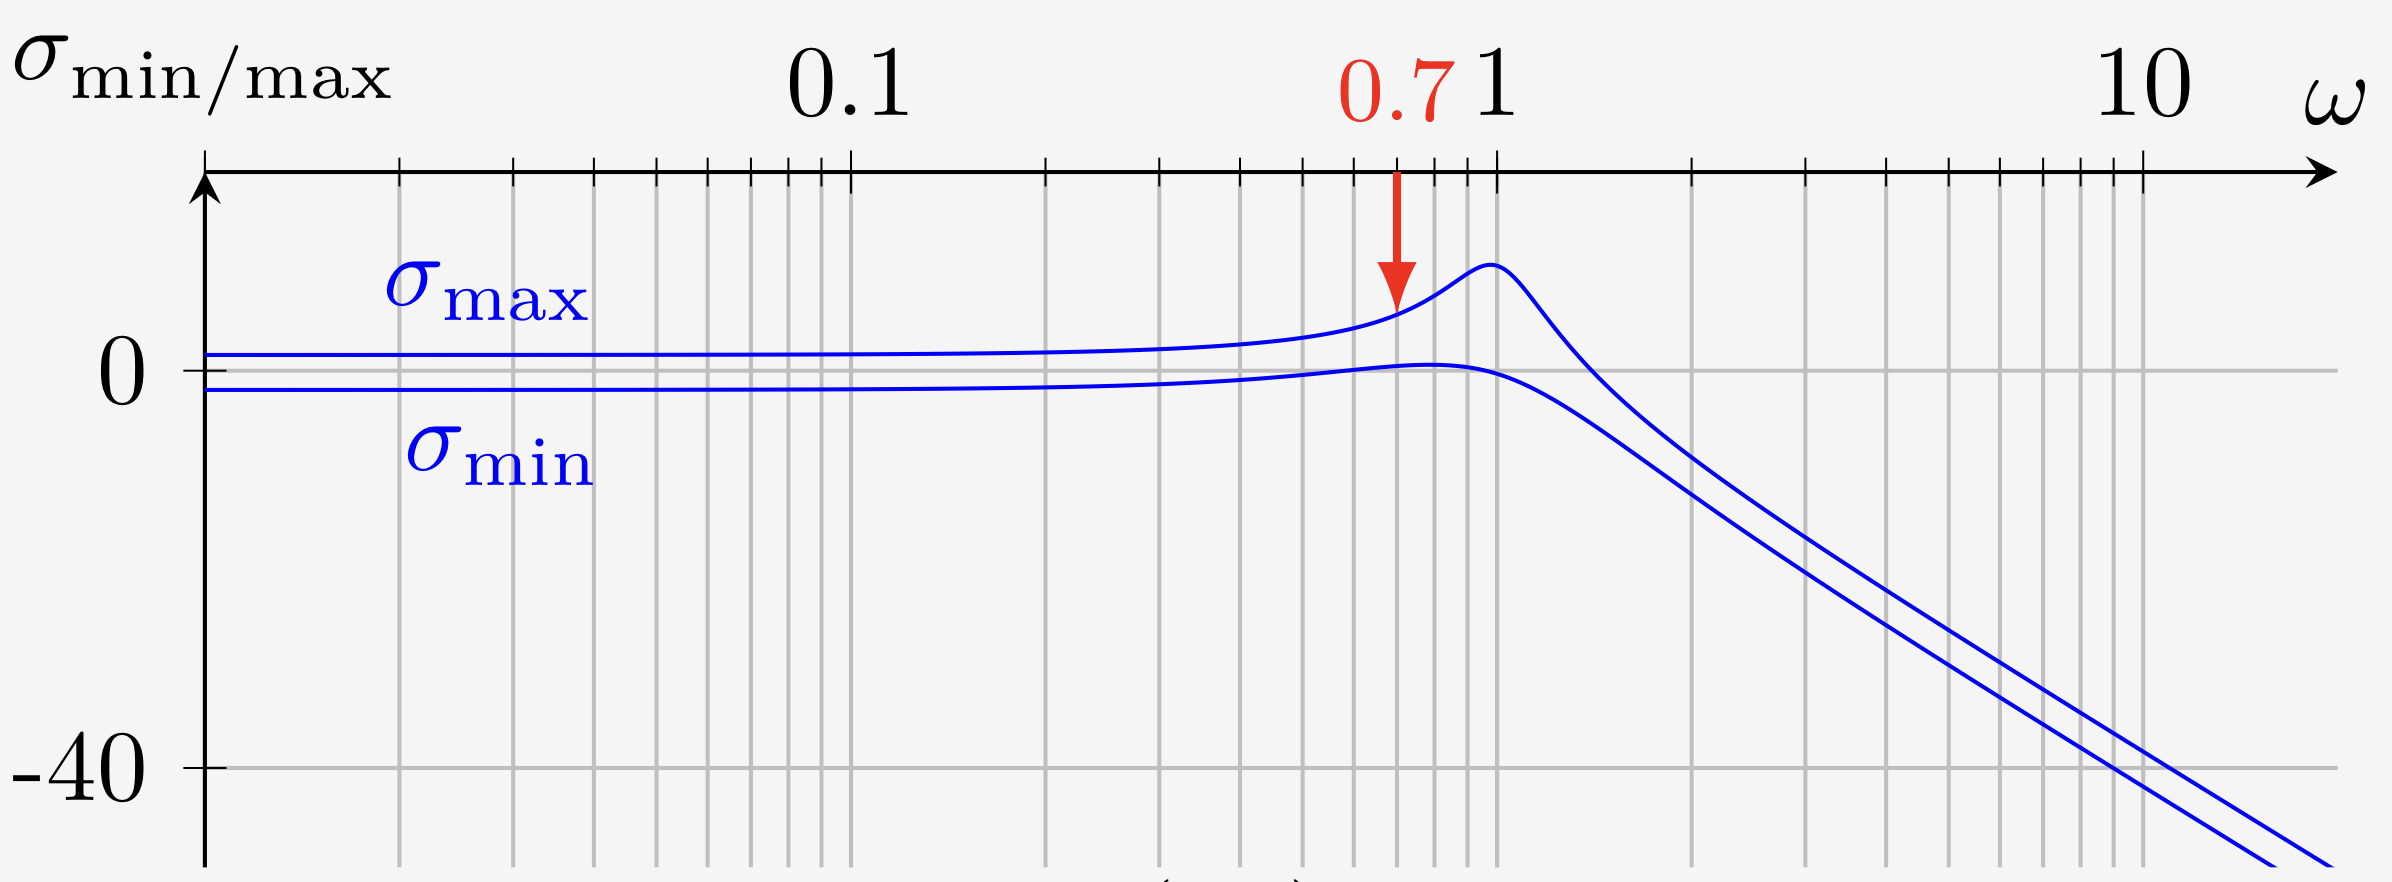
\includegraphics[width = 0.5\linewidth]{images/07/singular_val_plot.jpeg}
        \end{figure}
        
        Wir stellen fest, dass $\sigma_\textnormal{max}\big(P(j\cdot0.7)\big) = 1.914$. Die Ausgänge $y_1$ und $y_2$ werden je Amplituden $\nu_1$ und $\nu_2$ haben, die kleiner als 1.914 sind. Bei der maximalen Anregung wird die Norm  jedoch $\|\nu\| = 1.914$ sein.
        
        Um die Anregungsrichtung zu finden, bei der $\|\nu\|$ maxial wird, verwendet man die Singulärwertzerlegung der Matrix $P(j\cdot0.7)$:
        \begin{align*}
            P(j\cdot0.7) &= U\cdot\Sigma\cdot V^\top = \\ 
           &\begin{bmatrix}
           \textcolor{red}{-0.8724+0.3635j}  &   0.3089-0.1068j\\
           \textcolor{red}{-0.2167+0.2247j}  &   -0.6691+0.6675j
           \end{bmatrix}
           \cdot
           &\begin{bmatrix}
           \textcolor{blue}{1.914}    &   0\\
           0        &   1.056
           \end{bmatrix}
           \cdot\\
           &\begin{bmatrix}
           \textcolor{cyan}{-0.9344}  &   \textcolor{cyan}{-0.3525+0.0515j}\\
           0.3562   &   -0.9246+0.1351j
           \end{bmatrix}
        \end{align*}
        \textcolor{red}{Ausgangsrichtung der Maximalen Verstärkung} entspricht der ersten Spalte von $U$, die \textcolor{blue}{Maximale Verstärkung} entspricht dem höchsten Singulärwert, welcher an erster Stelle steht und die \textcolor{cyan}{Eingangsrichtung der maximalen Verstärkung} entspricht der ersten Zeile von $V^\top$. \big(MATLAB: \texttt{V(:,1)\big)}
        
        Die Maximale Richtung ist somit:
        \begin{gather*}
            \zeta_\textnormal{max} = 
            \begin{bmatrix}
            -0.9344\\ -0.3525+0.0515j
            \end{bmatrix}
            =
            \begin{bmatrix}
            e^{j\pi} & 0\\
            0 & e^{j2.9965}
            \end{bmatrix}
            \cdot
            \begin{bmatrix}
            0.9344\\ 0.3562
            \end{bmatrix}\\
            \Rightarrow u(t) = 
            \begin{bmatrix}
            0.9344\cdot\cos\left(0.7\cdot t + \pi\right)\\
            0.3562\cdot\cos\left(0.7\cdot t + 2.9965\right)
            \end{bmatrix}
        \end{gather*}
        
        \begin{figure}[H]
            \centering
            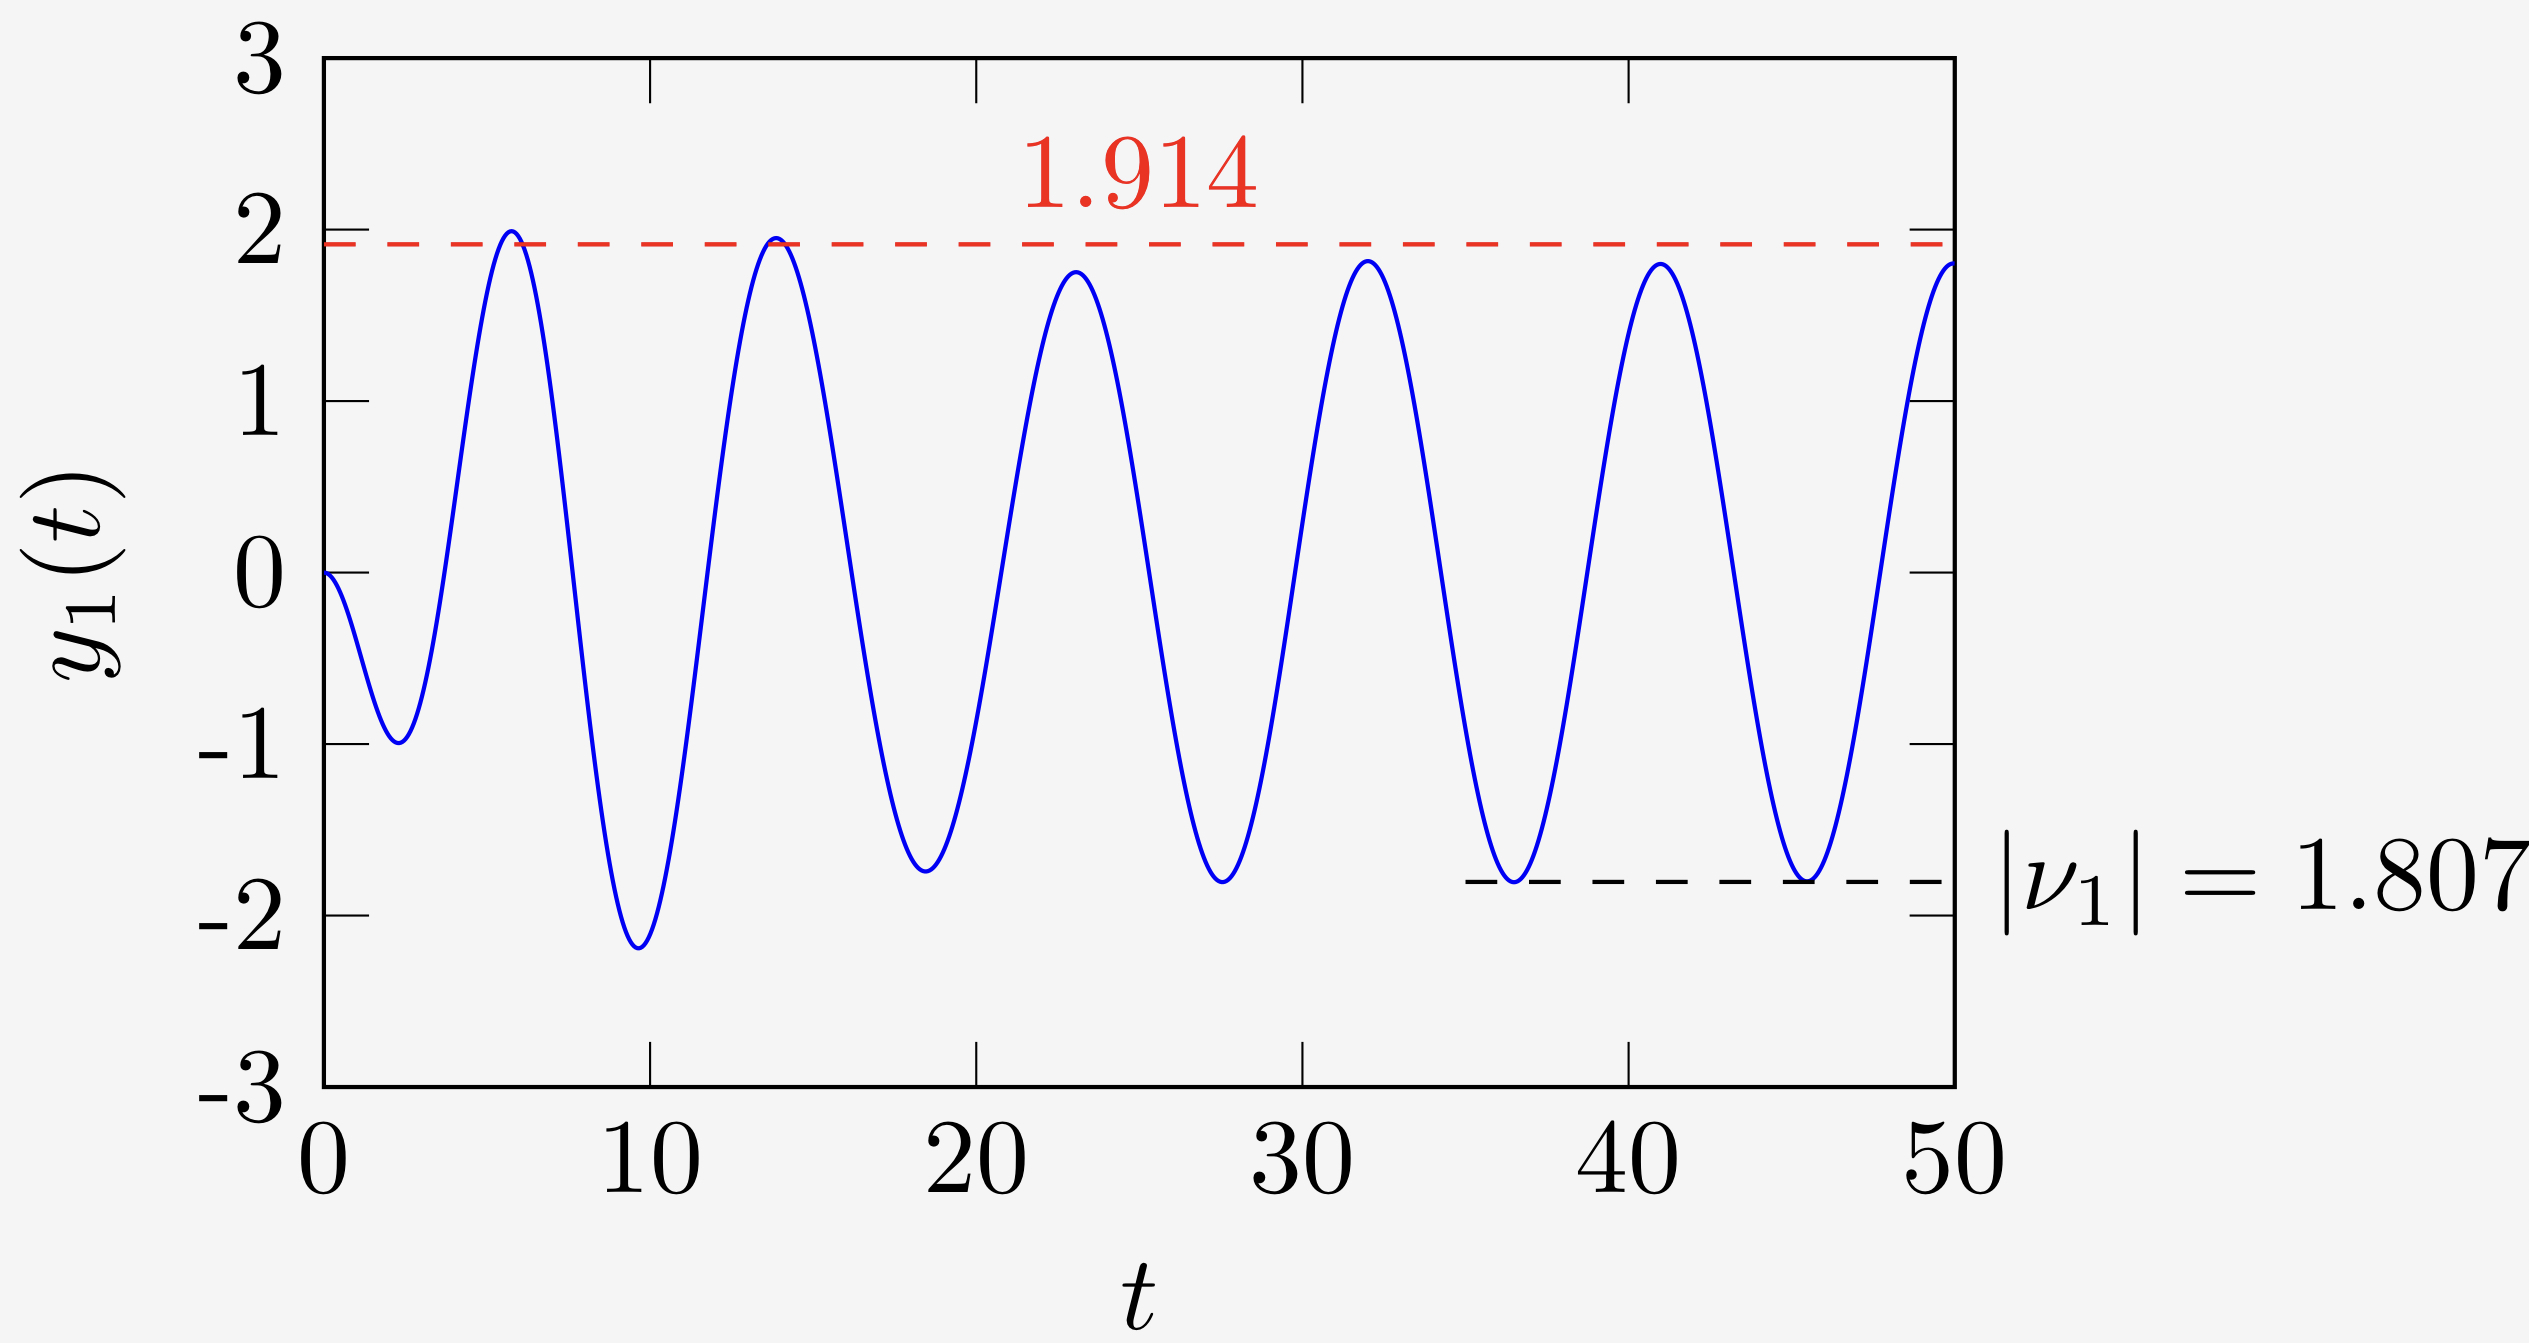
\includegraphics[width = 0.45\linewidth]{images/07/freq_resp_bsp_1.jpeg}
            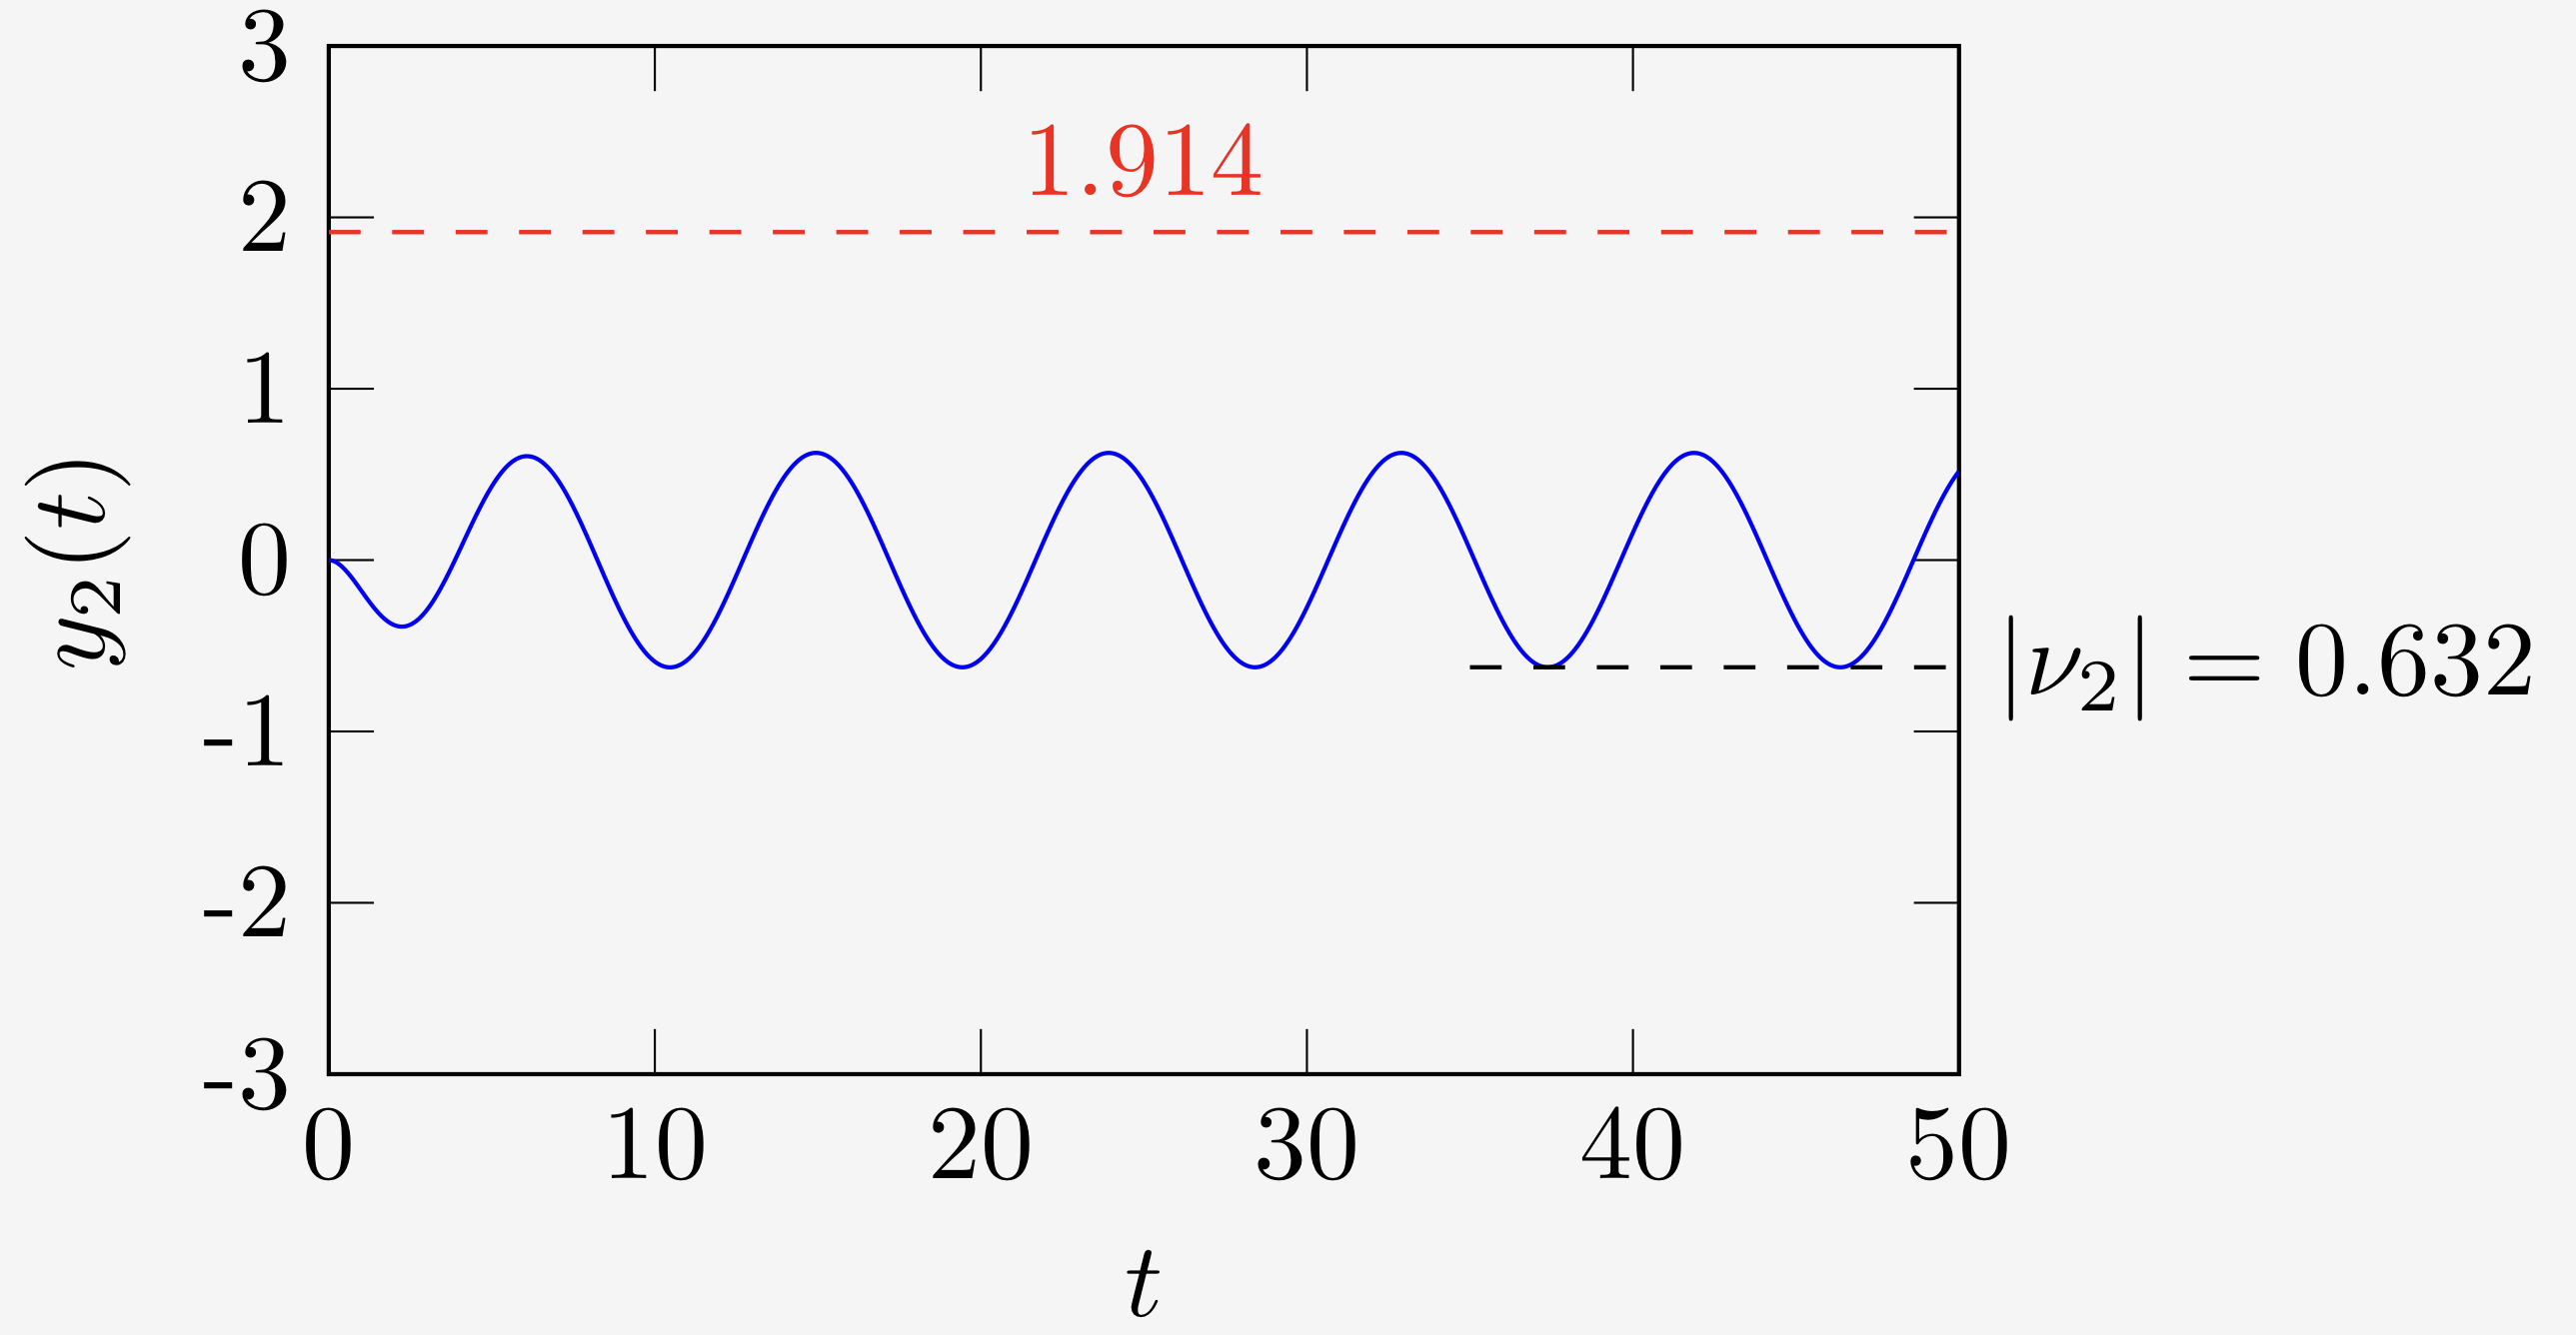
\includegraphics[width = 0.45\linewidth]{images/07/freq_resp_bsp_2.jpeg}
            \caption{Simulation des Systems mit Eingangssignal der Maximalen Verstärkung}
        \end{figure}
        
        \textbf{Bemerkungen:}
        \begin{itemize}
            \item $|\nu_1| < \sigma_\textnormal{max} \quad\Rightarrow\quad y_{1,\infty} < \sigma_\textnormal{max}$
            \item $|\nu_2| < \sigma_\textnormal{max} \quad\Rightarrow\quad y_{2,\infty} < \sigma_\textnormal{max}$
            \item $\sqrt{|\nu_1|^2 + |\nu_2|^2} = 1.914 = \sigma_\textnormal{max}$ (Da maximale Richtung angeregt)
        \end{itemize}
    \subsection{Singulärwertverläufe als Werkzeug}
    Singulärwertverläufe sind das MIMO Analogon zu den SISO Bode-Plots. Der entscheidende Unterschied ist aber, dass man bei den SWV keine Information über die Phase hat und dass sie \textbf{worst-case Abschätzungen} sind im gegensatz zu effektiven Verstärkungen im Bode-Plot.
    
    Da bei Singulärwertverläufen die euklidische Norm des Eingans $= 1$ ist, \textbf{muss die euklidische Norm des Ausgangsvektors} $\mathbf{\in [\sigma_\textnormal{min},\sigma_\textnormal{max}]}$ \textbf{sein!}
    
    Die Singulärwertverläufe können für beliebige Übertragungsfunktionen ($S(s),\, T(s),\, L(s),\, Q(s)$) erstellt werden:
    \begin{align*}
        T(s) &= \big(I + P(s)\cdot C(s))\big)^{-1} \cdot P(s) \cdot C(s)\\
        S(s) &= \big(I + P(s)\cdot C(s))\big)^{-1}\\
        Q(s) &= I + P(s)\cdot C(s) \qquad\textnormal{(Return Difference)}
    \end{align*}
    
    Mit der Definition der Systemnorm
    \begin{equation*}
        \|G(s)\|_\infty = \max_\omega\bigg(\max_i \sigma_i\big(G(s)\big)\bigg),
    \end{equation*}
    hat dann z.B. die Sensitivität eine veranschulichende Interpretation: Die Systemnorm $\|S(s)\|_\infty$ ist die maximal zu erwartende/worst-case Verstärkung des Störsignals.
    
    \begin{figure}[H]
        \centering
        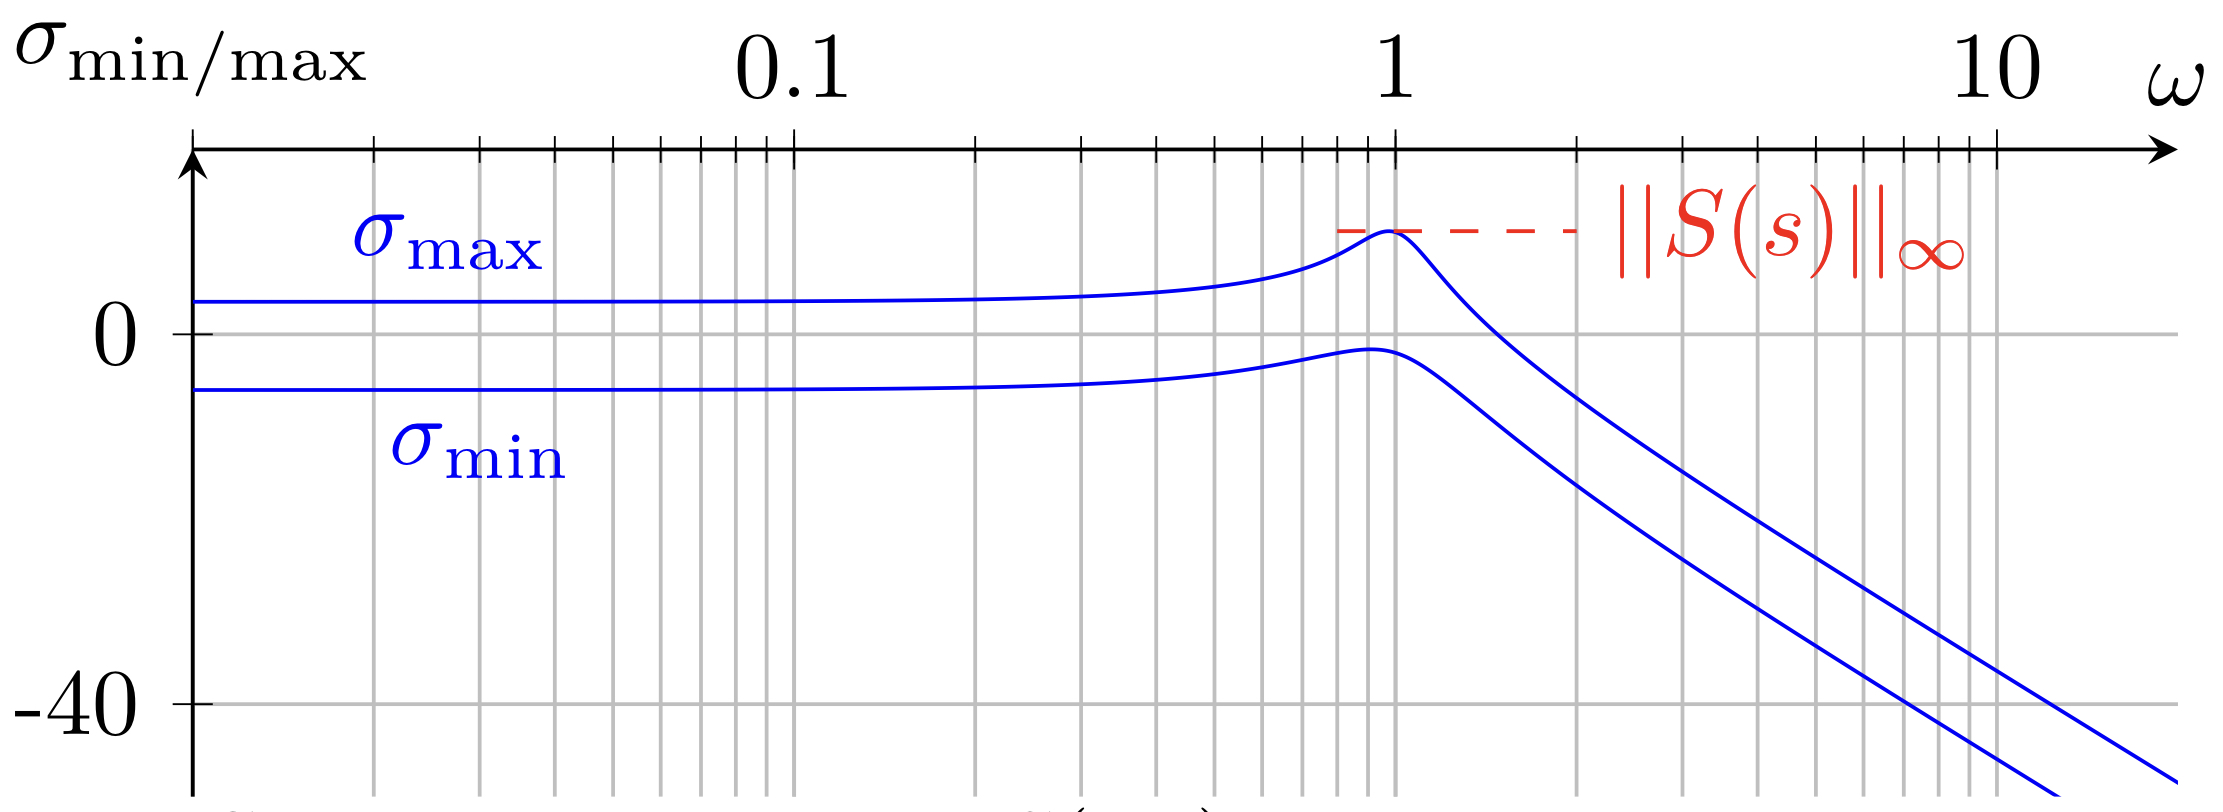
\includegraphics[width = 0.6\linewidth]{images/07/sysnorm.jpeg}
    \end{figure}
    Bei einer kleinen Systemnorm $\|S(s)\|_\infty$ weiss man, dass man eine gute Störungsunterdrückung hat.
    
    Die \textbf{Return Difference} gibt ein Mass für die Robustheit des Regelkreises:
    \begin{equation*}
        \colorboxed{red}{
        \mu_\textnormal{min} = \min_\omega \Big( \min_i\sigma_i\big\{I + L(\jw) \big\} \Big)
        }
    \end{equation*}
    
\vfill\null\columnbreak
\section{LQR}
    \subsection{Infinite Horizon LQR Formulierung}
    Der LQ-Regler beruht auf einem intuitiven Ansatz bei dem man beliebig einen Trade-off zwischen Regelfehler und Regelaufwand wählt. 
    
    LQR ist eine Abkürzung für \textit{linear quadratic regulator}. 
    
    \textbf{Linear:} da das System linear ist:
    \[\frac{d}{dt}x(t) = A\cdot x(t) + B\cdot u(t),\ x(t) \in \mathbb{R}^n,\ u(t) \in \mathbb{R}^m\]
    \textbf{Quadratic:} Definition einer  \textit{quadratischen} Kostenfunktion J:
    \[
    \colorboxed{red}{
    J(u(t)) = \int_0^\infty\Big(x(u(t))^T\cdot Q\cdot x(u(t)) + u(t)^T \cdot R \cdot u(t)\Big)dt
    }
    \]
    der optimale Eingnang $u^*(t)$ minimiert die Kostenfunktion J:
     \[u^*(t) = \arg\min J(u(t))\]
     Die Zustände $x(t)$ und Eingänge $u(t)$ werden in Optimierungsproblem mit $Q$ und $R$ gewichtet, wobei 
     \[Q=Q^T \in \mathbb{R}^{n\times n},\ Q \succeq 0,\ \textnormal{und}\ R = R^T \in \mathbb{R}^{m\times m},\ R\succ 0\]
     Die Definitheit der Matrizen $Q$ und $R$ ist notwendig, damit das Argument des Integrals quadratisch konvex ist.
     Somit ist das Minimum von $J(u)$ einzigartig, falls es existiert.
    
    \textbf{Regulator:}
    der Reglerlösst das \textit{regulator} Problem:
    \[\lim\limits_{t \to \infty}x(t)=0\]
    
    $\boxed{Q\uparrow \widehat{=}\, R \downarrow}$ \textbf{Cheap Control.} Je grösser $Q$ relativ zu $R$, desto teurer ist es wenn $x(t)$ nicht im Ursprung ist. Das System wird schnell an den Ursprung geregelt, um die Kosten tiefstmöglich zu halten. Dabei wird $u(t)$ jedoch betragsmässig gross sein.
    
    $\boxed{Q\downarrow \widehat{=}\, R \uparrow}$ Je grösser $R$ relativ zu $Q$, desto teurer ist es viel Energie mit den Ausgangsgrössen auszugeben. Das System wird langsam (mit betragsmässig kleinem Regelsignal $u(t)$) in den Ursprung geregelt.
    
    \textbf{Note:} eine Erhöhung der Eigenwerte von $Q$ hat den gleichen Effekt wie eine Reduzierung derer von $R$. Die relative Grösse ist von Relevanz.
    
    \subsubsection{Lösung der LQR-Formulierung}
        Die Lösung der LQR-Formulierung ist eine \textbf{lineare Zustandsrückführung} und lautet  
        \[
        \colorboxed{red}{
        u^*(t) = -K\cdot x(t),\ \textnormal{wobei}\ K = R^{-1}\cdot B^T\cdot\Phi
        }
        \]
        
        Note: Die Matrix $K$ ist \textbf{statisch}, sie muss für gegebene $\{A,B,Q,R\}$ nur einmal berechnet werden.
    
    \subsubsection{algebraische Riccati Gleichung}
        Dabei ist $\Phi$ die einzige positive Lösung der algebraischen Riccati Gleichung 
        \begin{equation*}
        \colorboxed{red}{
        \Phi\cdot B \cdot R^{-1}\cdot B^T \cdot \Phi-\Phi \cdot A - A^T \cdot \Phi - Q = 0
        }
        \end{equation*}
        
        Wählt man 
        \[Q = \overline{C}^T\cdot \overline{C},\quad \overline{C}\in\mathbb{R}^{p\times n}\ \textnormal{wobei}\ p = \operatorname{rank}(Q),\]
        dann ist $\Phi$ garantiert positiv definit, falls $\{A,B\}$ \textbf{steuerbar} und $\{A,\Bar{C}\}$ \textbf{beobachtbar} sind. Diese Bedingungen sind hinreichen aber nicht notwendig.
        
        Note:
        \begin{enumerate}
            \item  Die Matrix $\overline{C}$ hat nichts mit der Matrix C zu tun. Falls jedoch $\overline{C} = C$ gewählt wird, wird $||y(t)||_2$ in der Kostenfunktion berücksichtigt.
            \item Der open loop gain lautet $L_{LQR}(s) = K\cdot (sI-A)^{-1}\cdot B$ 
            \begin{figure}[H]
                \centering
                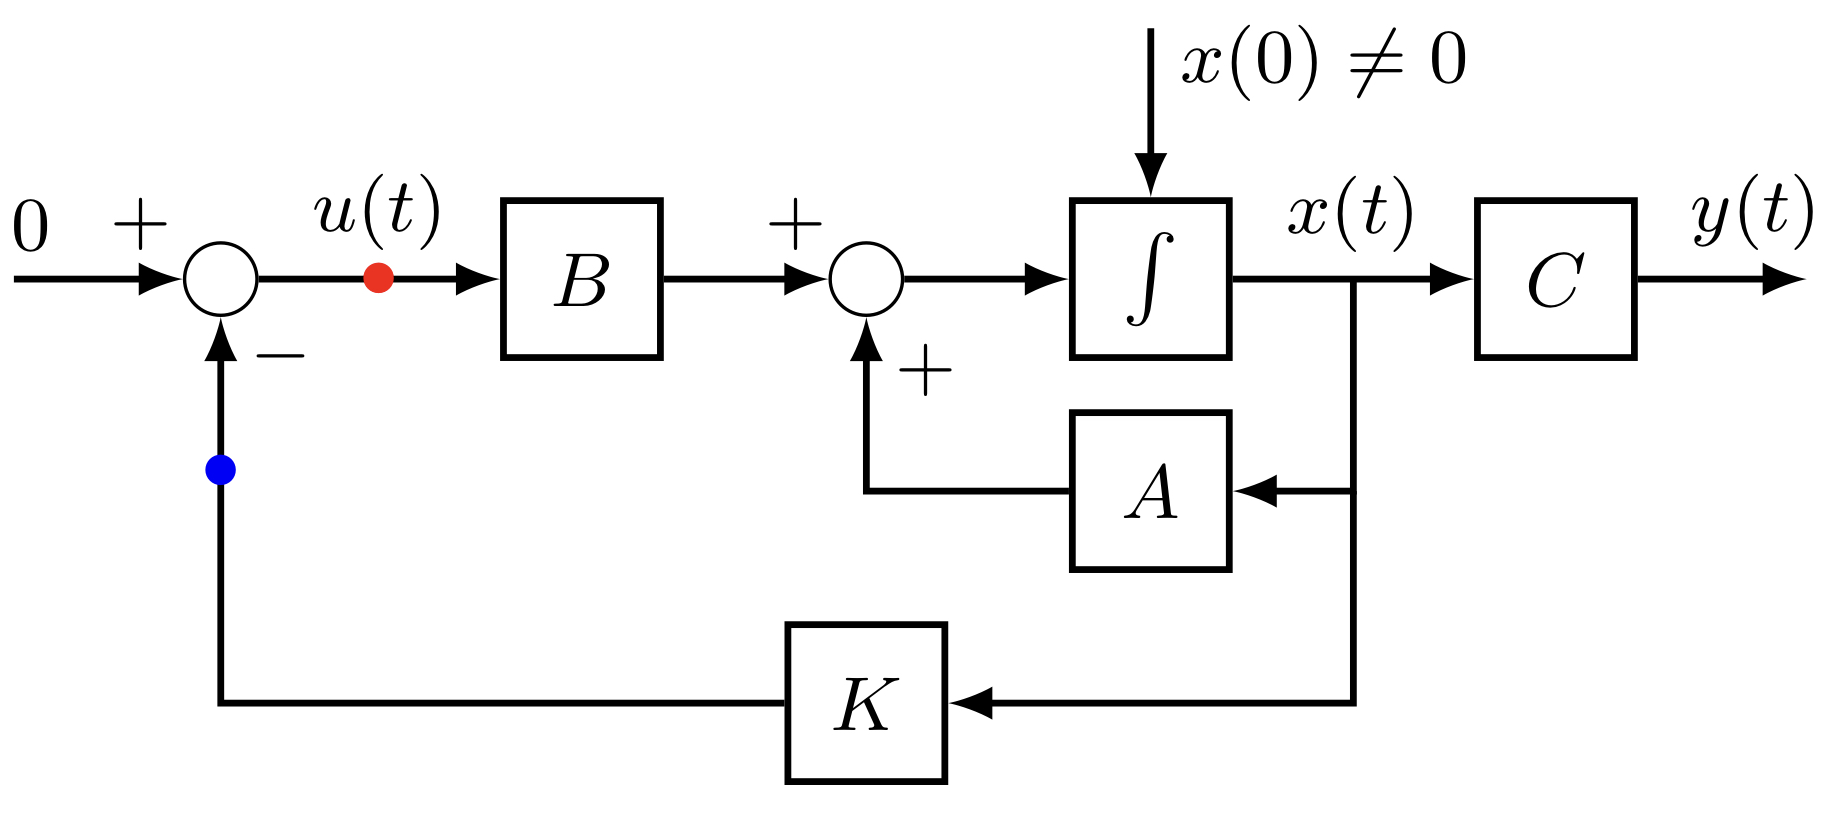
\includegraphics[width = 0.5\linewidth]{08/L_lqr.jpeg}
                \caption{$L_{\textnormal{LQR}}$ von $\textcolor{red}{\bullet}  \rightarrow \textcolor{blue}{\bullet}$}
            \end{figure}
            \item Robust Stability ist auch bei Modellunsicherheit gewährleistet.
        \end{enumerate}
    
    \subsubsection{Eigenschaften von Infinite Horizon Reglern}
        \textbf{Stabilität:}
        Die Matrix $A-B\cdot K$ des geschlossenen Regelkreises ist \textbf{garantiert Hurwitz} (stabil).
        \begin{equation*}
            \colorboxed{red}{\Dot{x}(t) = \big(A - B\cdot K\big) \cdot x(t)}
        \end{equation*}
    
        \textbf{Robustheit:}
        Für die Wahl $R=r\cdot I$ hat die minimum return difference $\mu_{min}$ folgende Eigenschaft:\[\mu_{min,LQR} = \min_{\omega}\Big(\min_{i}\ \sigma_i(I+L_{LQR}(j\omega))\Big) \geq 1 \]
        
        Im SISO-Fall lässt sich diese Eigenschaft folgendermassen darstellen.
        Dies garantiert eine Verstärkungsreserve von $\gamma \in [\,0.5, \infty)$ und eine Phasenreserve von $\varphi \geq 60^\circ$
        
        \begin{figure}[H]
            \centering
            \includegraphics[width=0.5\linewidth]{08/SISO_Robustheit.jpg}
            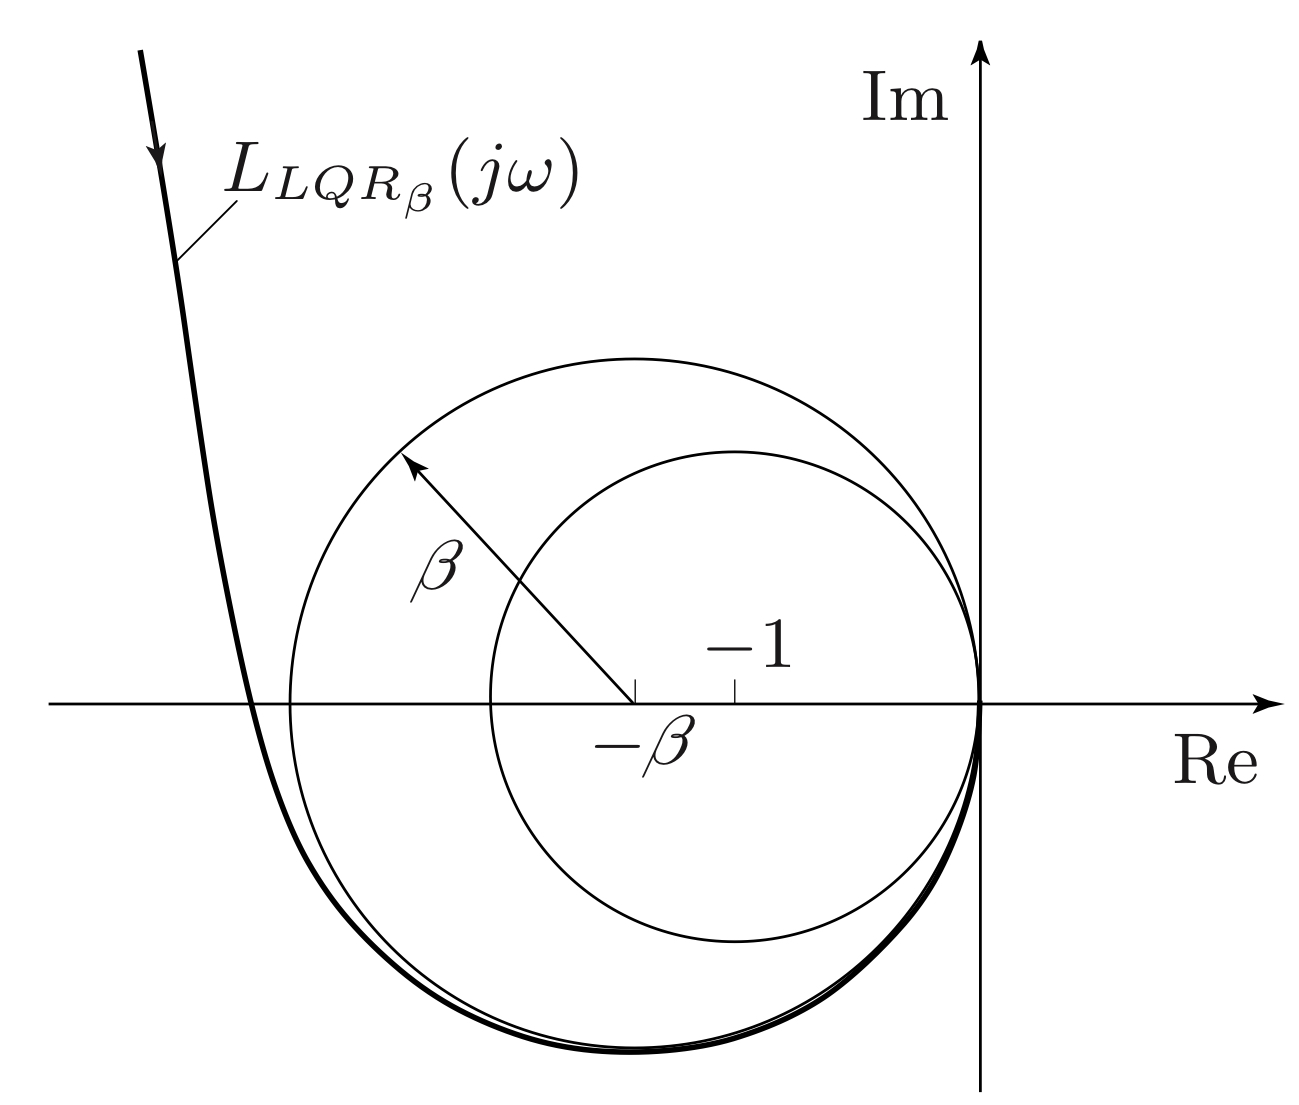
\includegraphics[width=0.4\linewidth]{08/beta_robust.jpeg} 
        \end{figure}
        % \begin{figure}[H]
        %     \centering
        %     \includegraphics[width = 0.6 \linewidth]{images/08/SISO_Robustheit.jpg}
        % \end{figure}
    
        Durch modifizieren der Riccati-Gleichung mit $\beta > 1$ wie folgt:
        \[\frac{1}{\beta}\cdot\Phi_\beta\cdot B\cdot R^{-1}\cdot B^T\cdot \Phi_\beta - \Phi_\beta \cdot A - A^T\cdot \Phi_\beta-Q = 0\]
        
        so resultiert die Lösung $\Phi_\beta$. Damit wird der Regelkreis noch robuster, da dann gilt: 
        
        \[\mu_{min,LQR}=\min_\omega\Big(\min_{i}\ \sigma_i(\beta I+L_{LQR}(j\omega))\Big) \geq \beta \]
        
        Das heisst, der Nyquist-Plot tritt nie in den um $-\beta +j\cdot0$ zentrierten Kreis mit Radius $\beta$ ein.
        
    \subsection{Lösung der LQR-Formulierung}
    Die Lösung der LQR-Formulierung ist eine lineare Zustandsrückführung und lautet  
    \[
    \colorboxed{red}{
    u^*(t) = -K\cdot x(t),\ \textnormal{wobei}\ K = R^{-1}\cdot B^T\cdot\Phi
    }
    \]
    
    Note: Die Matrix $K$ ist statisch, sie muss für gegebene $\{A,B,Q,R\}$ nur einmal berechnet werden.

    \subsubsection{algebraische Riccati Gleichung}
        Dabei ist $\Phi$ die einzige positive Lösung der algebraischen Riccati Gleichung 
        \[
        \colorboxed{red}{
        \Phi\cdot B \cdot R^{-1}\cdot B^T \cdot \Phi-\Phi \cdot A - A^T \cdot \Phi - Q = 0
        }
        \]
        Wählt man \[Q = \overline{C}^T\cdot \overline{C},\quad \overline{C}\in\mathbb{R}^{p\times n}\ \textnormal{wobei}\ p = \operatorname{rank}(Q),\]
        dann ist $\Phi$ garantiert positiv definit, falls $\{A,B\}$ steuerbar und $\{A,\Bar{C}\}$ beobachtbar sind. Diese Bedingungen sind hinreichen aber nicht notwendig.
        
        Note:\begin{enumerate}
                \item  Die Matrix $\overline{C}$ hat nichts mit der Matrix C zu tun. Falls jedoch $\overline{C} = C$ gewählt wird, wird $||y(t)||_2$ in der Kostenfunktion berücksichtigt.%, da:
                % \[ x^T\cdot Q \cdot x = x^T \cdot\overline{C}^T\cdot \overline{C} \cdot x = x^T \cdot C^T \cdot C \cdot x = y^T \cdot y = \|y\|_2.\]
                \item Die Dynamik des geregelten Systems lautet $\dot x = (A-BK)x$. Die Matrix $A-BK$ ist garantiert Hurwitz. D.h. der geschlossene Regelkreis ist asymptotisch stabil.
                \item Der open loop gain lautet $L_{LQR}(s) = K\cdot (sI-A)^{-1}\cdot B$ ``Der open loop gain betrachtet den offenen Pfad vom roten zum blauen Punkt, wobei beim blauen Punkt aufgeschnitten wir" \textbf{Bild hinzfügen?}
            \end{enumerate}
    
    \subsection{Folgeregelung}
        % Die LQR-Formulierung löst nur das Regulator Problem, wir können die Linearität des Systems ausnützen um einen gewünschten Zustand $x_{\infty}$ anzusteuern. 
        
        \textbf{Zur Erinnerung:} Ein lineares System beschreibt die Dynamik der Differenzen. Wir können den Ursprung des Systems demnach in einen neuen Punkt verschieben, mit den Definitionen $\Delta x = x -x_\infty$ und $\Delta u = u - u_\infty.$ Die Dynamik des Systems in den neuen Variablen lautet:
        \[\Delta\dot x = A \cdot \Delta x + B \cdot \Delta u,\]
        Wobei die Kostenfunktion nun auch angepasst werden muss:
        \[J(\Delta u) = \int^\infty_0(\Delta x^T(t) \cdot Q \cdot \Delta x(t) + \Delta u^T(t) \cdot R \cdot \Delta u(t)) dt \]
        das neue Regulator Problem lautet somit: 
        \[\lim\limits_{0 \to \infty} \Delta x(t) = 0 \]
        Somit linearisiert man das System um einen neuen Punkt $\{x_\infty,u_\infty\}$. Dies eintspricht bei einem linearen System ein Ursprungsverschiebung. Die Lösung des Regulatorsproblems der Dynamik der Differenz lautet nun
        \[\Delta u = u - u _\infty = -K \cdot \Delta x = -K \cdot ( x-x_\infty)\]
        Der Eingang auf das originale System $\dot x = A\cdot x + B \cdot u$ lautet somit:
        \[u = u_\infty - K \cdot (x-x_\infty),\]
        wobei $u_\infty$ ein statisches feedforward Signal ist, welches das System am gewünschten Punkt $x_\infty$ hält. 
        
        Im Gleichgewicht sind alle Ableitungen null: \[ 0 = A\cdot x_{\infty} + B \cdot u_\infty\]
        
        \begin{figure}[H]
            \centering
            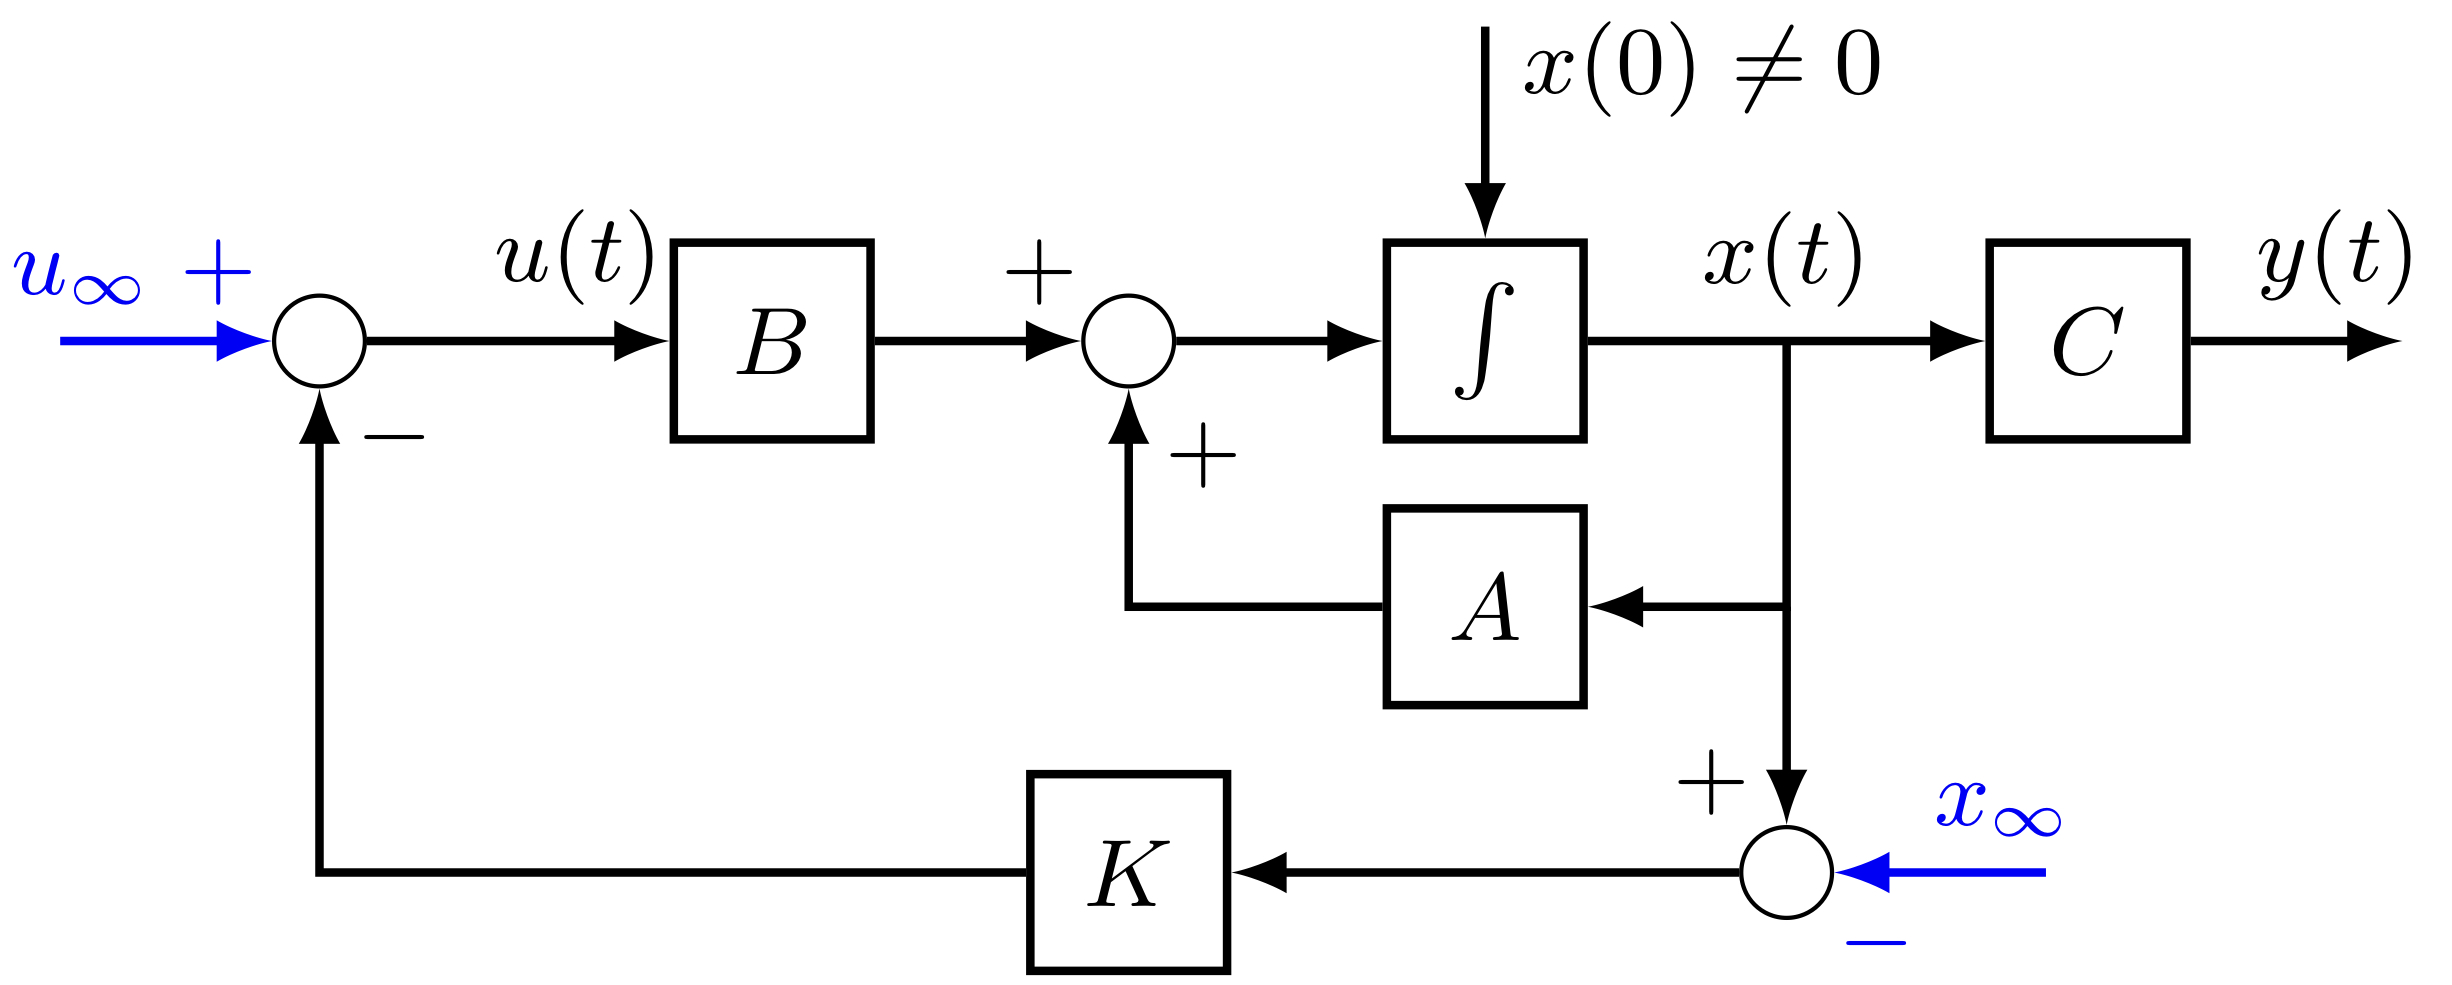
\includegraphics[width = 0.8\linewidth]{images/08/LQR_Folgeregelung.jpeg}
        \end{figure}
        
        \textbf{Bemerkungen}:
        \begin{itemize}
            \item Die Stellgrösse $u_\infty$ ist statisch für eine statische Referenz $x_\infty$. 
            \item Die Folgeregelung mit feedforward kann keine Störungen unterdrücken.
            \end{itemize}
    \subsection{Störungsunterdrückung - LQRI}
Um Störung ud Modelfehler zu unterdrücken greift man zum LQRI, welcher zusätzlich zum standard LQR-Regler noch ein integratives Verhalten eingeführt wird. Um Störungen zu unterdrücken wird das Integral des Fehlers als neuer Zustand definiert: \[ v(t) = \int^t_0 e(\tau)d\tau = \int^t_0 (0-<(\tau))d\tau.\]
der neue Gesamtzustand lautet somit: \[\Tilde{x}(t) =\begin{bmatrix}
x(t) \\ v(t)
\end{bmatrix}\in \mathbb{R}^{n+m}\]

Die Ableitung des Zustands lautet
\begin{align*}
    \frac{d}{dt}\Tilde{x}(t) = \begin{bmatrix}A\cdot x(t) + B \cdot ( u(t) + w(t))\\-y(t)\end{bmatrix}\\
    = \underbrace{\begin{bmatrix}A&0\\-C & 0\end{bmatrix}}_{\Tilde{A}}\cdot\begin{bmatrix}x(t) \\v(t)\end{bmatrix}+\underbrace{\begin{bmatrix}B \\ 0 \end{bmatrix}}_{\Tilde{B}} \cdot(u(t)+w(t))
\end{align*}
Das neue System erfüllt im Gelichgewicht $\dot v = y(t) = 0$

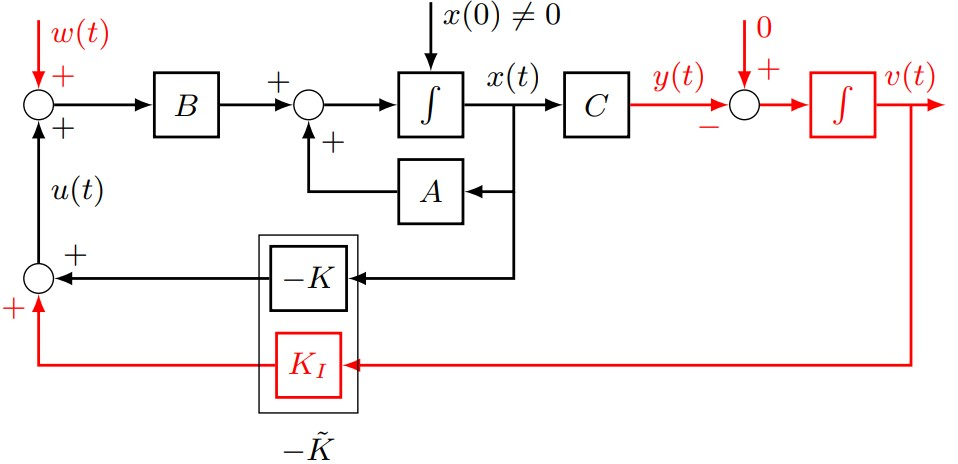
\includegraphics[width=0.8\linewidth]{images/08/LQRI.jpg}

Die Standard LQR Formulierung kann nun mit den Matrizen $\Tilde{A}$ und $\Tilde{B}$ gelöst werden, wobei die Dimension der $Q$ Matrix angepasst werden muss:
\[\Tilde{Q} =\begin{bmatrix} Q & 0 \\ 0 & Q_I\end{bmatrix},\ Q_I = \begin{bmatrix}
    \gamma_1 & 0 & \dots & 0 \\
    0 & \gamma_2 & \dots & 0\\
    \vdots & \vdots &\ddots &   \vdots\\
    0 & 0 & \dots &\gamma_m
\end{bmatrix}\]
Mit $Q_I$ kann man einstellen, wie stark die Integratoren wirken sollen. Die Lösung des LQRI-Problems lautet:
\begin{align*}
    \{\Tilde{A},\Tilde{B},\Tilde{Q},R\}\rightarrow \Tilde{K}=[\,K, - K_I]\, \in \mathbb{R}^{m\times(n+m)},\\
    u(t) = -\Tilde{K}\cdot\Tilde{x}(t) = u_K + u_{K_I} = -K\cdot x(t) + K_I\cdot v(t).
\end{align*}
note: \begin{itemize}
    \item Die Matrix $\Tilde{K}$ ist statisch, sie muss für gegebene $\{\Tilde{A},\Tilde{B},\Tilde{Q},R\}$ nur einmal berechnet werden.
    \item Mit $Q = C^T \cdot C$ kann wiederum direkt $y(t)$ in der Kostenfunktion berücksichtigt werden. 
\end{itemize}
    \subsection{Folgeregelung mit Störungsunterdrückung}
    Wenn man den LQRI-Ansatz um die feedforward Signale $u_\infty$ und $x_\infty$ erweitert, um auf eine Referenz mit Störungsunterdrückung zu regeln.
    
    Da nun auf eine Referenz geregelt wird, muss der Fehler im Zustand $ v(t)$ neu definiert werden: 
    \[v(t) = \int^t_0e(\tau)d\tau = \int^t_0(r(\tau)-y(\tau))d\tau\]
    Die Ableitung des Zustands lautet nun: 
    \begin{align*}
        \frac{d}{dt}\Tilde{x}(t) = \begin{bmatrix}A\cdot x(t) + B \cdot ( u(t) + w(t))\\r(t)-y(t)\end{bmatrix}\\
        = \underbrace{\begin{bmatrix}A&0\\-C & 0\end{bmatrix}}_{\Tilde{A}}\cdot\underbrace{\begin{bmatrix}x(t) \\v(t)\end{bmatrix}}_{\Tilde{B}}+\begin{bmatrix}B \\ 0 \end{bmatrix} \cdot(u(t)+w(t))+\begin{bmatrix}0 \\I\end{bmatrix}\cdot r(t).
    \end{align*}
    Die Lösung des Problems folgt:
    \begin{align*}
        \{\Tilde{A},\Tilde{B},\Tilde{Q},R\}\rightarrow \Tilde{K}=[\,K, - K_I]\, \in \mathbb{R}^{m\times(n+m)},\\
        u(t) = u_\infty-K\cdot(x(t)-x_\infty)+K_I\cdot v(t).
    \end{align*}
    
    \begin{figure}[H]
        \centering
        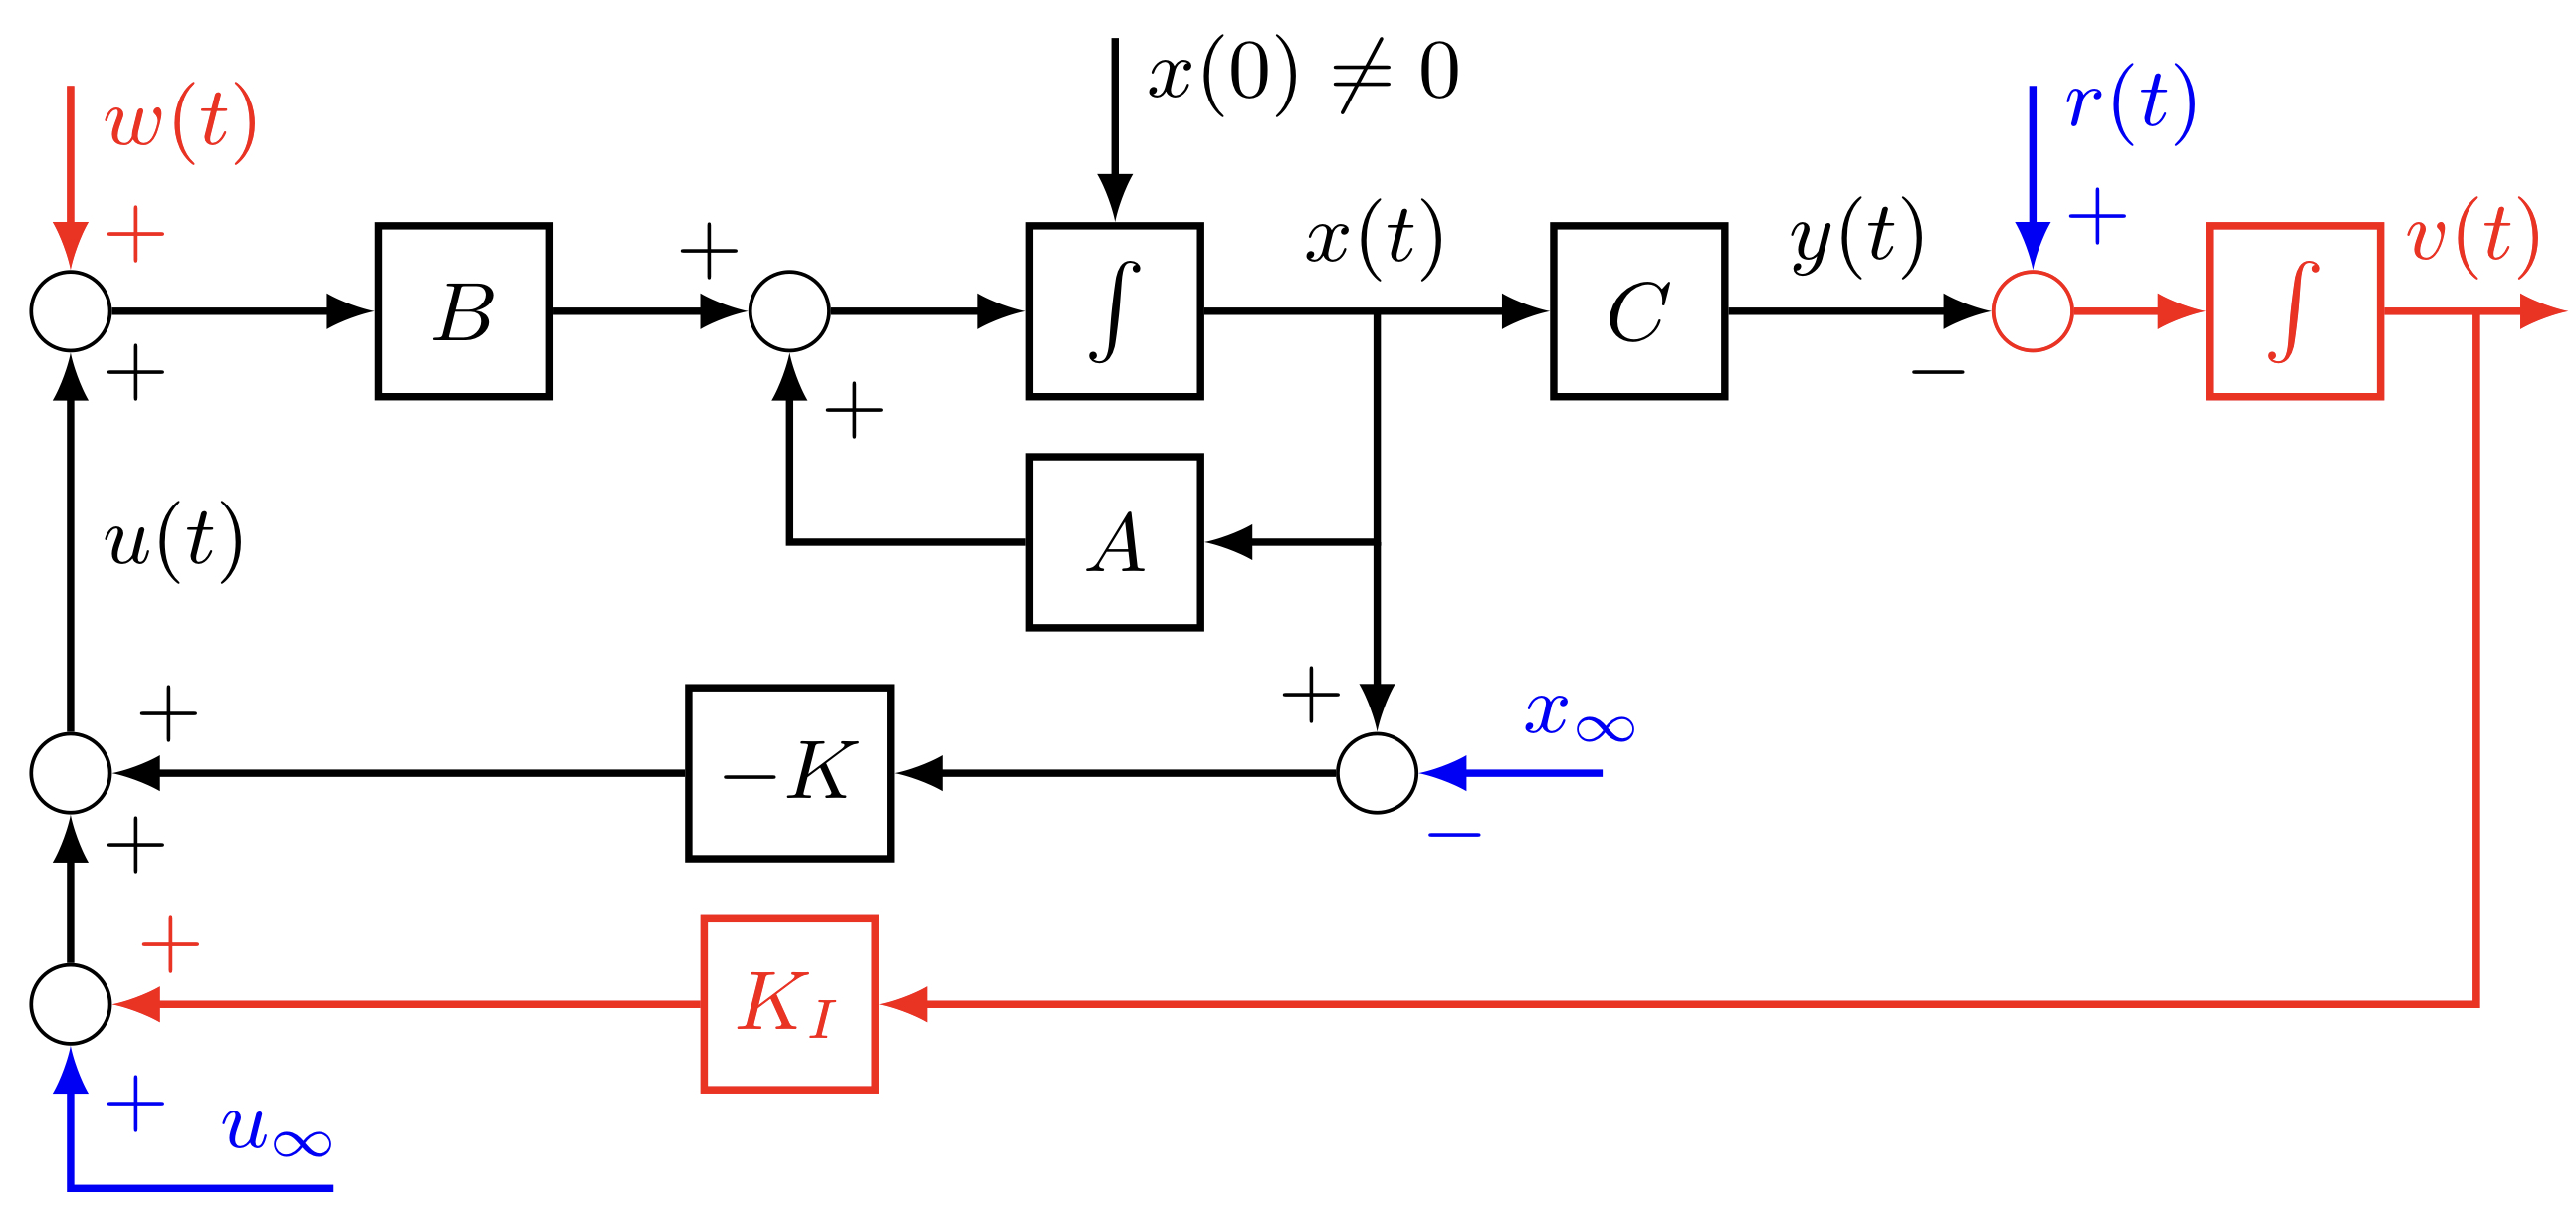
\includegraphics[width = 0.7\linewidth]{images/08/LQR_Folgereg_distreject.jpeg}
    \end{figure}
    Dieser Regler würde auch ohne Feedforward Teil $\{u_\infty(r(t)), x_\infty(r(t))\}$ funktionieren, wäre aber deutlich langsamer.


    \subsection{Finite Horizon LQR}
Das Integral der Kostenfunktion geht im Gegensatz zur Standardformulierung nur über ein Zeitintervall $t_a$ bis $t_b$. Dementsprechend lautet die Kostenfunktion:
\[J(u) = x^T(t_b)\cdot P \cdot x(t_b) + \int_{t_a}^{t_b}(x^T\cdot Q(t)\cdot x+u^T\cdot R(t)\cdot u) dt.\]
Mit der Kostenmatrix $ P \in \mathbb{R}^{n \times n}, P = P^T \succeq 0$ wird eine Abweichung des finalen Zustands $ x(t_b)$ vom Ursprung bestraft. Das System kann in diesem Fall zeitinvariant sein: \[\frac{d}{dt}x(t) = A(t)x(t)+B(t)u(t),\ x(t) \in \mathbb{R}^n,\ u(t) \in \mathbb{R}^m,\ x(t_a)=x_a\]
Die Lösung der finite Horizon Formulierung lautet:
\[u(t) = -K(t)x(t),\ \text{wobei } K(t)=R^{-1}(t)B^T(t)\Phi(t).\]
Die Matrix  $\Phi(t)$ ist die Lösung der differential matrix Riccati Gleichung:
\[\frac{d}{dt}\Phi(t)=\Phi(t)B(t)R^{-1}(t)B^T(t)\Phi(t) -\Phi(t)A(t)-A^T(t)\Phi(t)-Q(t)\]
wobei $\Phi(t)$ durch Rückwärtsintegration von $\Phi(t_b) = P$ gefunden werden kann.
\textbf{Bemerkungen:}
\begin{itemize}
    \item Die Matrix $K(t)$ ist zeitabhängig. Sie muss entsprechend der Zeitabhängigkeit der Matrizen $\{A(t),B(t),Q(t),R(t)\}$
    \item Die Matrix P ist eine neue Tuninggrösse.
    \item Die Matrix $K(t)$ ist nur für das Zeitintervall $ t in [\,t_a,t_b]\,$ gültig. Für Zeiten $t > t_b$ muss $K(t)$ neu evaluiert werden.
    \item asymptotische Stabilität kann nicht garantiert werden, da für $t>t_b$ nicht optimiert wird.
\end{itemize}
\subsubsection{Folgeregelung}
Zusätzlich zur zeitinvarianten Dynamik wird nun der zeitvariante Ausgang eingeführt: \[y(t) = C(t) \cdot x(t)\]
Die Kosten die über ein Zeitintervall $[\,t_a,t_b]\,$ integriert werden lauten: 

\begin{align*}J(u)&=(r(t_b)-y(t_b))^T\cdot P\cdot(r(t_b)-y(t_b))\\
&+\int_{t_a}^{t_b}((r(t)-y(t))^T \cdot Q(t)\cdot (r(t)-y(t))+u(t)^T\cdot R(t) \cdot u(t))dt
\end{align*}

Die Lösung der finiten horizon Folgeregelung lautet: \[u(t) = -K(t)\cdot x(t) + v(t)\]
\textbf{Bemerkungen:}

\begin{itemize}
    \item Die Referenztrajektorie $r(t)$ ist eine Wahl, die vor dem Lösen des Optimierungsproblems festgelegt wird.
    \item Die Matrix $K(t)$ ist zeitabhängig. Sie muss ensprechend der Zeitabhängigkeit der Matrizen $\{A(t),B(t),Q(t),R(t)\}$ berechnen werden. 
    \item Die Matrix K(t) ist nur für das Zeitintervall $t \in [\,t_a,t_b]\,$ gültig. Für Zeiten $t>t_b$ muss $K(t)$ neu evaluiert werden.
    \item $v(t)$ ist ein zeitabhängiges feedforward Signal, welches nur im Zeitintervall $t \in [\,t_a,t_b]\,$ für eine spezifische Referenz $r(t)$ gültig ist.
\end{itemize}
    
\vfill\null\columnbreak
\section{Zustandsbeobachter}
    \subsection{Zustandsbeobachter}
    Lineare Zustandsregler (wie z.B. LQR) basieren auf der Kenntnis von $x(t)$. Das ist praktisch aber nicht umsetzbar. Deshalb benutzt man \emph{Zustandsbeobachter} um durch $u(t)$ und $y(t)$ eine Schätzung $\widehat{x}(t)$ zu erhalten.
    
    \subsection{Luenberger Beobachter}
        Man will eine Beobachterdynamik $\frac{d}{dt}\widehat{x}(t)$ s.t. der Beobachtungsfehler $e(t) = x(t) - \widehat{x}(t)$ asymptotisch zu Null konvergiert $\displaystyle\lim_{t\to\infty}e(t) = 0$.
        
        \begin{align*}
            \frac{d}{dt}\widehat{x}(t) &= \widehat{A}\cdot\widehat{x}(t)+\widehat{B}\cdot u(t) + L\cdot\big(y(t)-\widehat{y}(t)\big)\\
            \widehat{y}(t) &= \widehat{C}\cdot\widehat{x}(t)
        \end{align*}
        
        \begin{figure}[H]
            \centering
            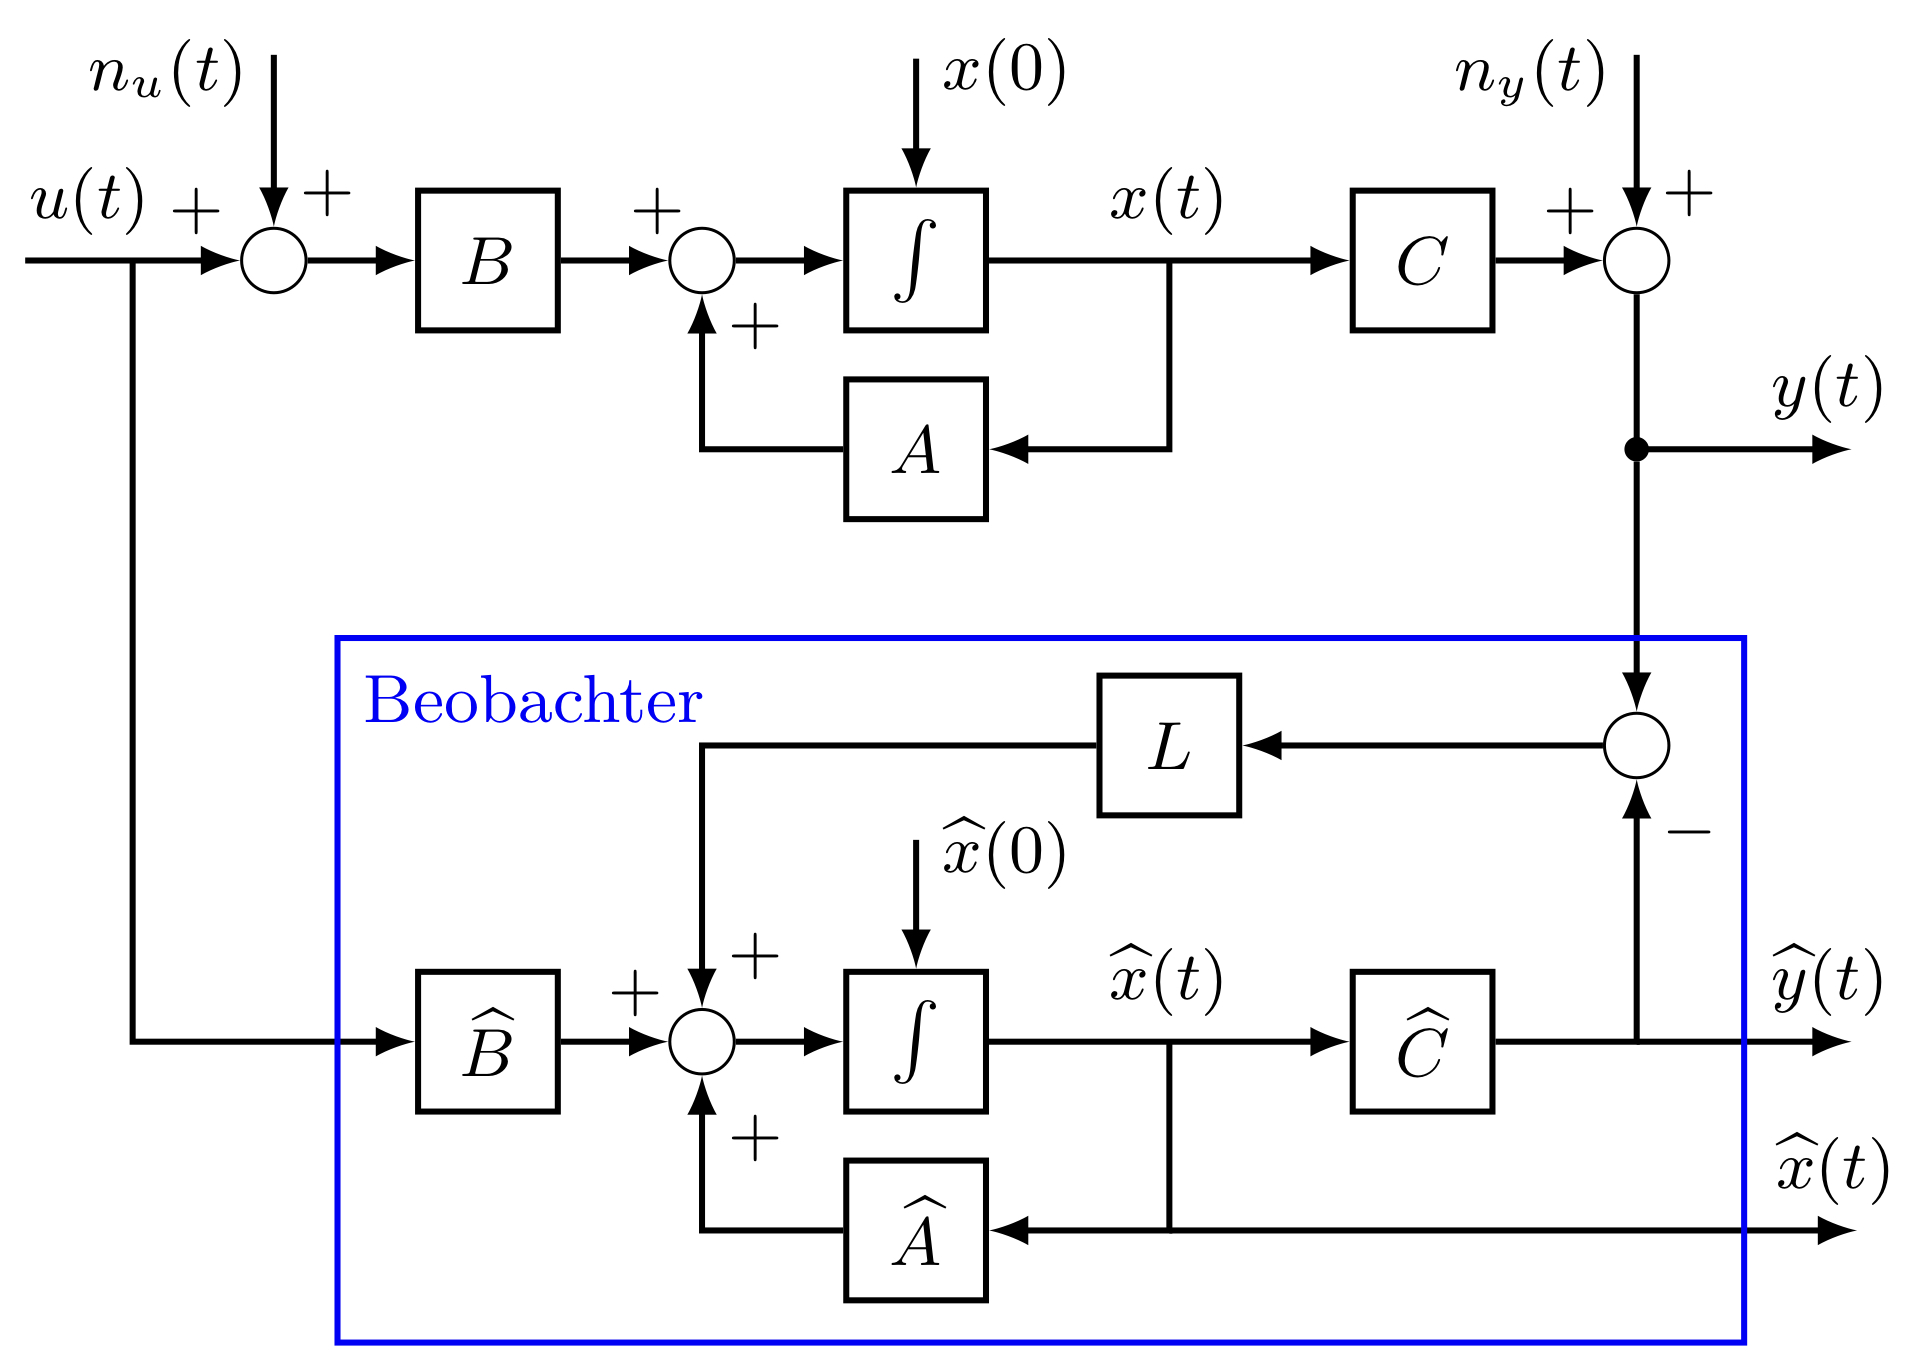
\includegraphics[width = 0.7\linewidth]{images/09/luenberger_obsv.jpeg}
            \caption{Blockdiagramm des Luenberger Observers}
        \end{figure}
        
        Unter der Annahme, dass ein perfektes Modell vorliegt \big(i.e. $\widehat{(\cdot)} = (\cdot)$\big) ergibt sich Folgende Fehlerdynamik:
        \begin{equation*}
            \colorboxed{red}{\frac{d}{dt}e(t) = \big(A- L\cdot C\big)\cdot e(t)},\quad e(0) = x(0)-\widehat{x}(0) \neq 0
        \end{equation*}
        Fehler konvergiert zu 0 falls $A- L\cdot C$ Hurwitz ist. Dies kann unter anderem durch zwei Arten erreichen:
             
        \subsubsection{Pole Placement}     
             Man platziert die gewünschten Polynome von Hand indem man $L$ durch folgende Gleichung bestimmt:
            \begin{equation*}
                \det\big(A-L\cdot C - \lambda I) \overset{!}{=} (\lambda_1 - \lambda)(\lambda_2 - \lambda)\dots(\lambda_n - \lambda) = 0
            \end{equation*}
            Dabei sind $\lambda_i$ die gewünschten EW. Die Einträge der Matrix $L$ folgen dann aus den Vergleichen mit den $\lambda_i$.
            
        \subsubsection{LQR Formulierung}
            Da die $L$ und $C$ Matrizen ``vertauscht'' sind für die LQR Formulierung und da gilt
            \begin{equation*}
                \operatorname{eig}(X) = \operatorname{eig}(X^\top),\quad X\in\mathbb{R}^{n\times n}
            \end{equation*}
            können wir mit LQR Formulierung für die Matrix $A^\top - C^\top\cdot L^\top$ die Matrix $L$ bestimmen, welche uns die Matrix $A-L\cdot C$ Hurwitz macht.
            
            Mit den Änderungen
            \begin{align*}
                A&\rightarrow A^\top, & B&\rightarrow C^\top\\
                Q = \Bar{C}^\top\cdot\Bar{C}&\rightarrow \Bar{B}\cdot\Bar{B}^\top & R= r\cdot I &\rightarrow q\cdot I\\
                K &\rightarrow L^\top & \Phi &\rightarrow \Psi
            \end{align*}
            foglt für die Lösung der LQR Formulierung:
            \begin{equation*}
            \colorboxed{red}{
            \begin{aligned}
                &L^\top = \frac{1}{q}\cdot C\cdot \Psi\\
                &\Psi \cdot C^\top\cdot\frac{1}{q}\cdot C\cdot \Psi-\Psi\cdot A^\top-A\cdot\Psi-\Bar{B}\cdot\Bar{B}^\top = 0
            \end{aligned}
            }
            \end{equation*}
            
            Falls die Matrizen $\{A,C\}$ beobachtbar und $\{A,\Bar{B}\}$ steuerbar sind, existiert eine eindeutige positiv definite Lösung $\Psi$.
            
            \textbf{Bemerkungen:}
            \begin{itemize}
                \item $L$ ist statisch (muss nur einmal berechnet werden)
                \item Matrizen $\Bar{B}$ und $q$ werden iterativ getunt bis Resultat zufriedenstellend ist.
                \item Falls $n_y\neq0$ ist $\frac{d}{dt}e(t)$ noch um $-L\cdot n_y(t)$ erweitert. $L$ kann nicht beliebig gross gewählt werden.
            \end{itemize}
            
            \begin{figure}[H]
                \centering
                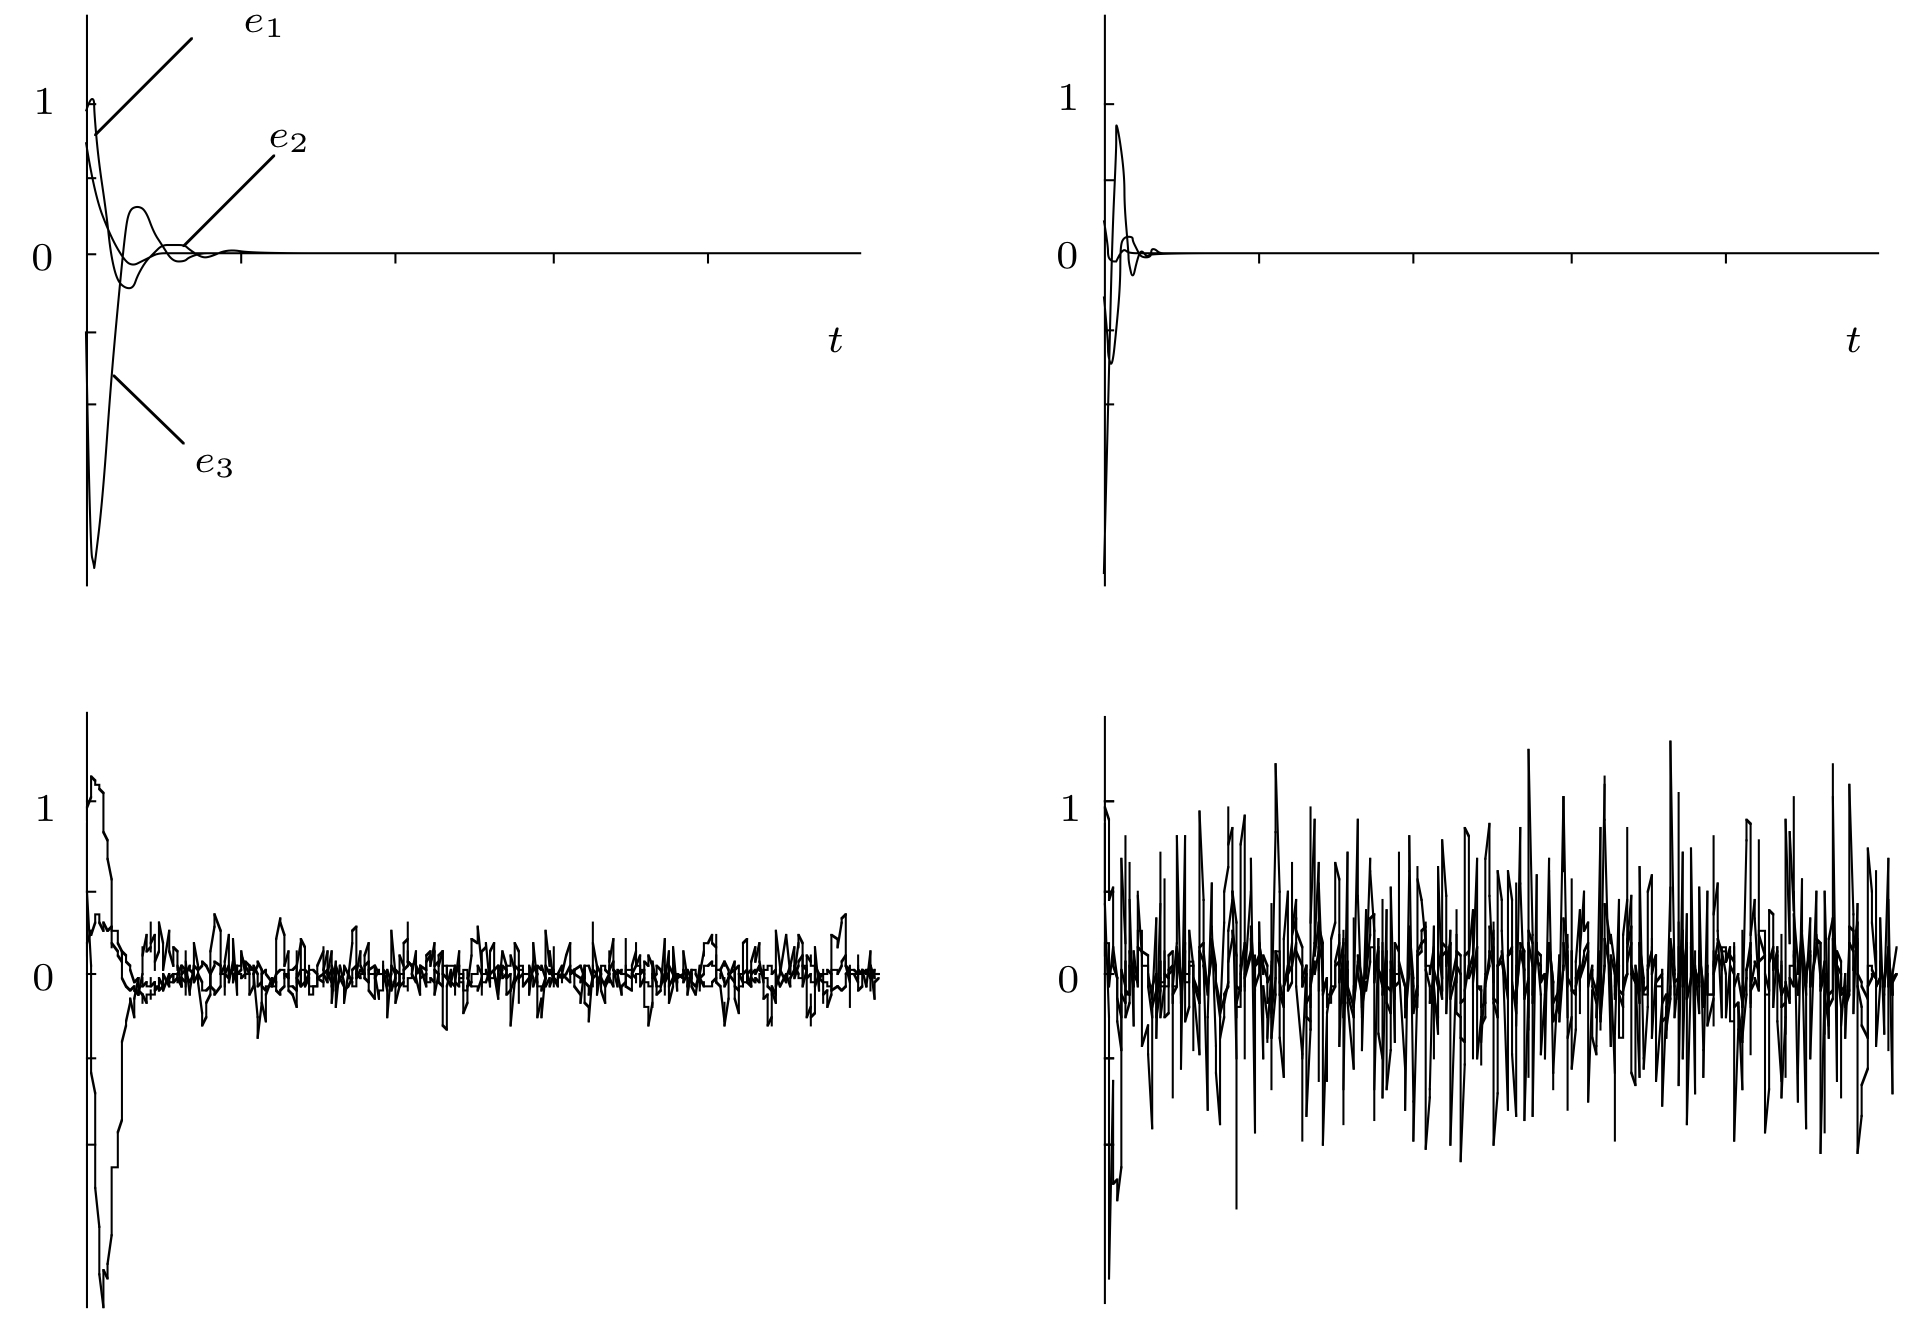
\includegraphics[width = 0.7\linewidth]{images/09/L_noise.jpeg}
                \caption{Links ``Langsames" $L$, Rechts ``schnelles" $L$}
            \end{figure}
    \subsection{Kalman Filter}
    Falls das Rauschen $n_u(t)$ und $n_y(t)$ \emph{Gausian zero mean white noise Signale} sind und die Varianz der Gaussverteilung bekannt ist, kann man ein ``optimales" $L$ finden, welches die Varianz des Beobachtungsfehlers $e(t)$ minimiert. Man änder dabei
    \begin{align*}
        \Bar{B}\cdot\Bar{B}^\top &\rightarrow B\cdot R_u \cdot B^\top\\
        q\cdot I &\rightarrow R_y
    \end{align*}
    
    \textbf{Bemerkungen:}
    \begin{itemize}
        \item $L_K$ ist statisch
        \item Kalman Filter hat keine tuning-Parameter mehr. $R_u,\, R_y$ werden durch statische Analyse bestimmt.
    \end{itemize}
    
    \subsection{Vergleich}
        Vergleich der LQR Formulierung der verschiedenen Methoden
        \begin{center}
            {\renewcommand{\arraystretch}{1.4}
            \begin{tabular}{c|c|c}
                LQR &   Luenberger  &   Kalman  \\
                \hline
                $K$ &   $L^\top$    &   $L^\top_K$\\
                \hline
                $A$ &   $A^\top$    &   $A^\top$\\
                $B$ &   $C^\top$    &   $C^\top$\\
                $Q = \Bar{C}^\top\cdot\Bar{C}$  &   $\Bar{B}\cdot\Bar{B}^\top$    &   $B\cdot R_u  \cdot B^\top$\\
                $R$ & $q\cdot I$    &   $R_y$\\
                $\Phi$ & $\Psi$     &   $P$
            \end{tabular}
            }
        \end{center}
    
\vfill\null\columnbreak
\section{LQG}
    \subsection{LQG-Regler}
    Die kombination eines LQR-Reglers und eines Luenberer-Observer nennt man \textit{LQG (Linear Quadratic Gaussian)}. Anstatt den realen Zustand $x(t)$ wird nun seine Schätzung $\widehat{x}(t)$ zurückgeführt.
    \begin{equation*}
        u(t) = -K\cdot\widehat{x}(t)
    \end{equation*}
    \begin{figure}[H]
        \centering
        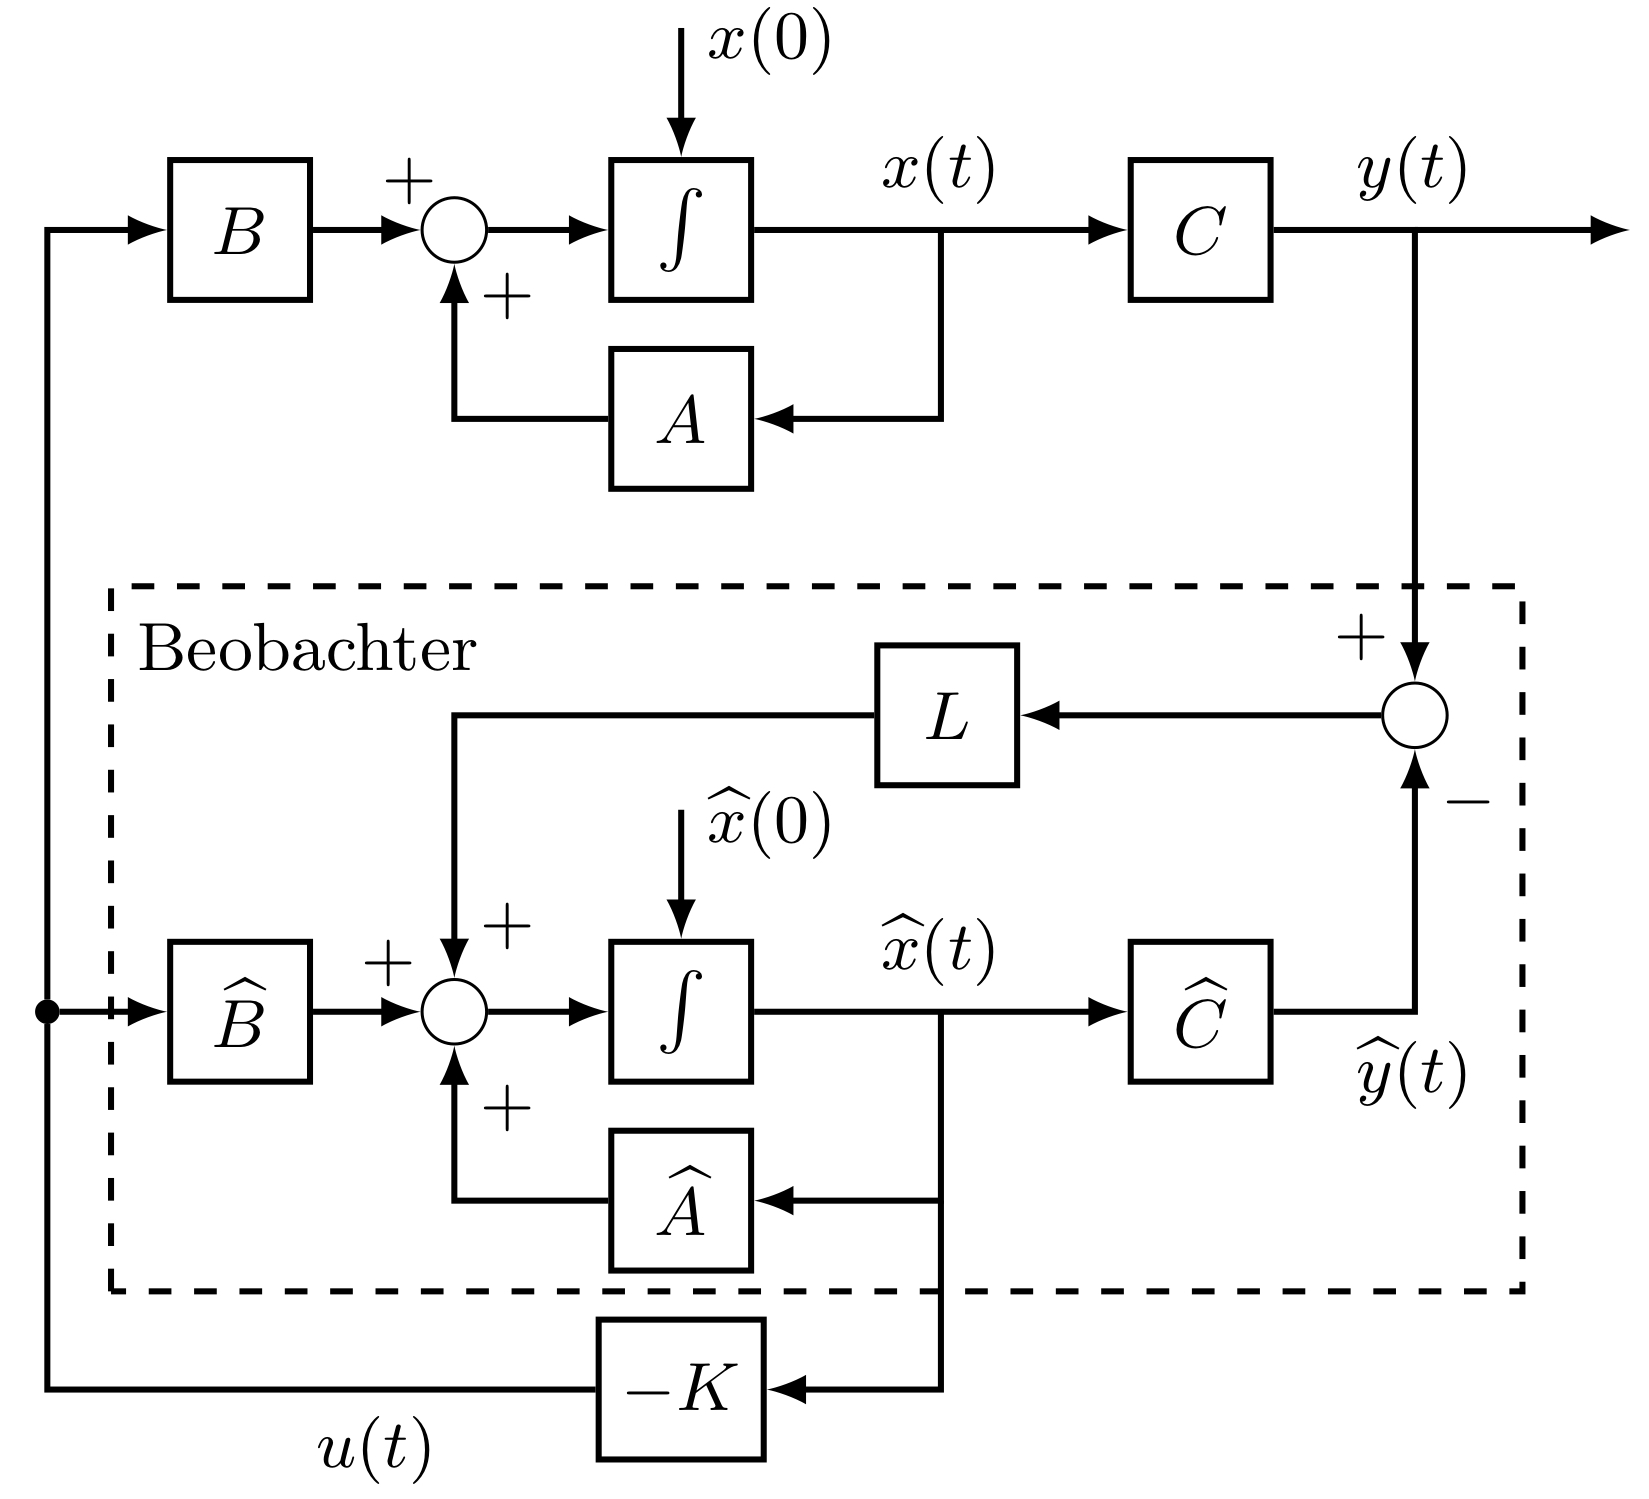
\includegraphics[width = 0.6\linewidth]{images/10/LQG_vanilla.jpeg}
        \caption{Blockdiagramm eines LQG-Reglers}
    \end{figure}
    
    \begin{figure}[H]
        \centering
        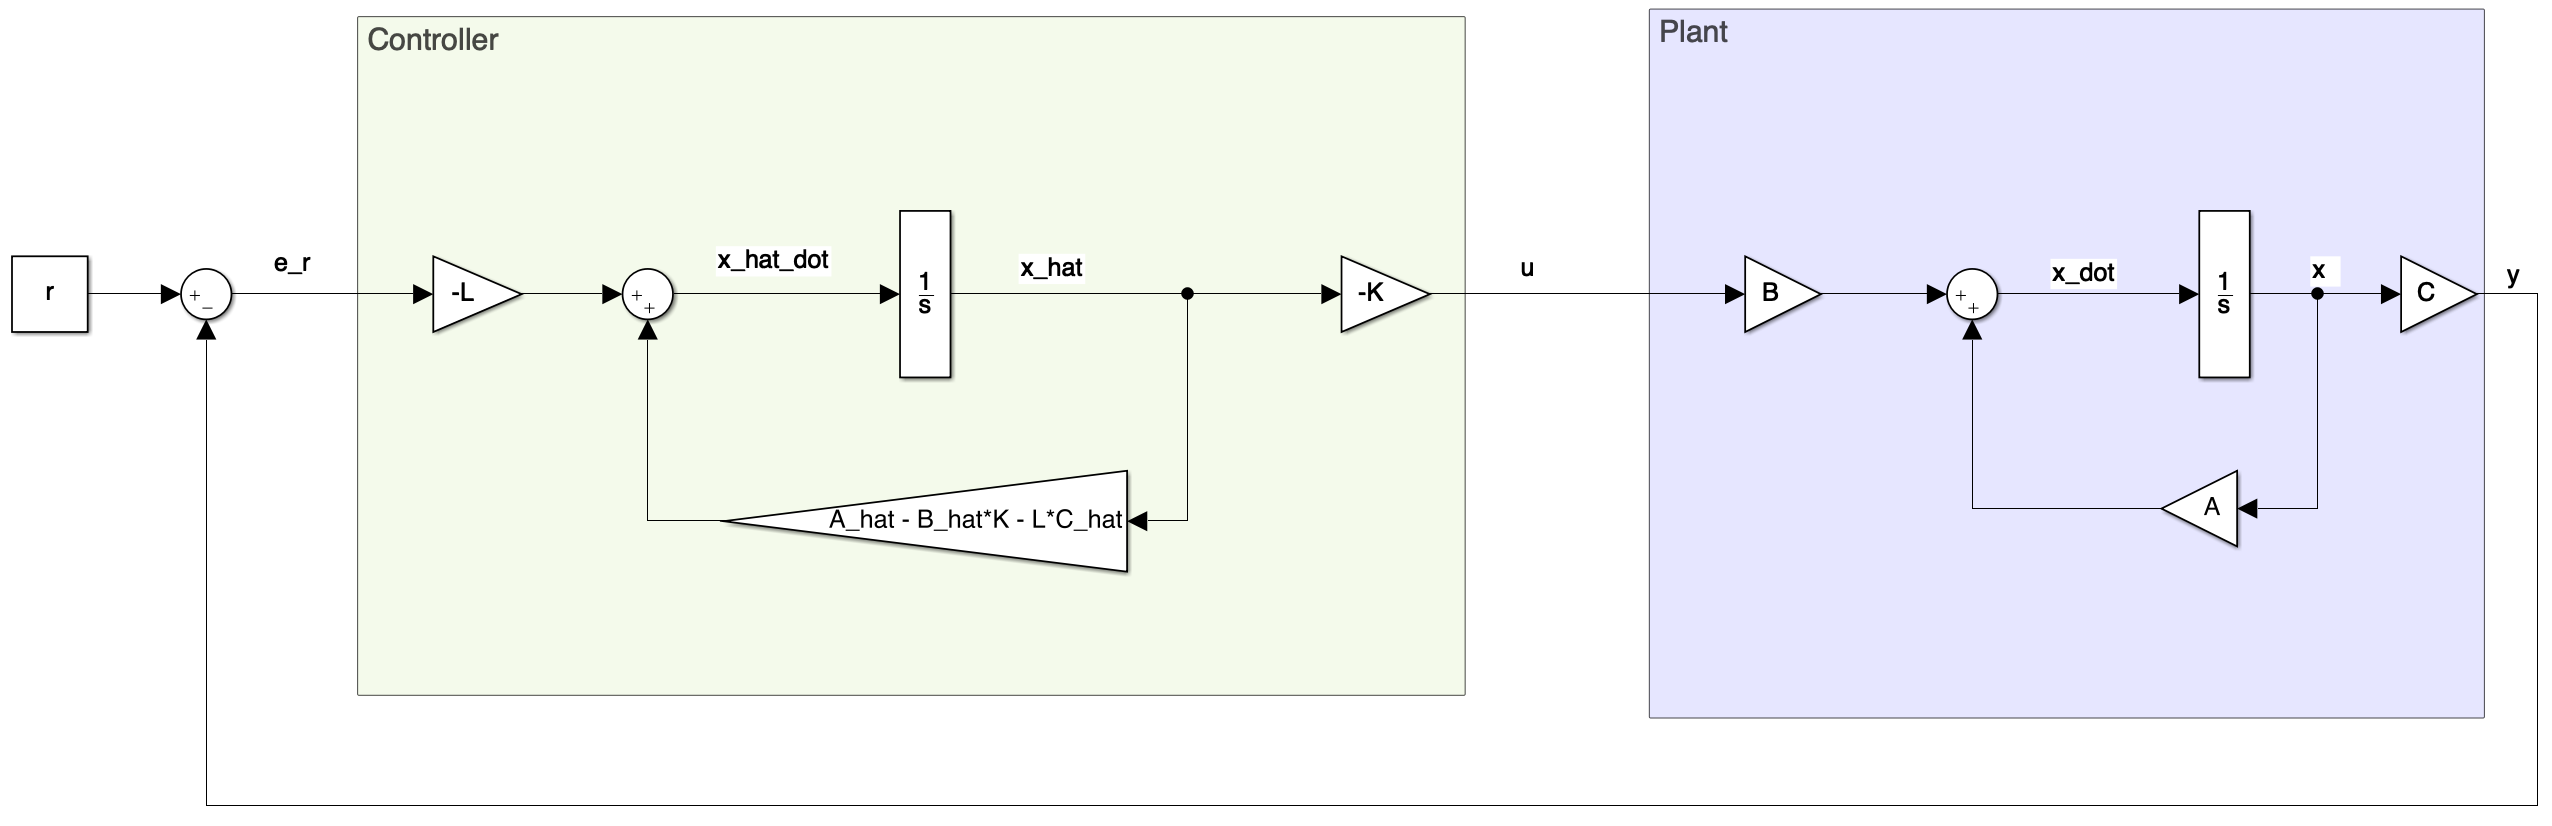
\includegraphics[width = \linewidth]{images/10/LQR_alt.png}
        \caption{Alternative Darstellung des LQR-Reglers}
    \end{figure}
    
\subsection{Stabilität des LQG}
    Unter der Annahme, dass die Matrizen $\{A, B, C\}$ exakt bekannt sind ergibt sich folgende Dynamik
    \begin{equation*}
        \Tilde{x}(t) = \begin{bmatrix}x(t)\\\widehat{x}(t)\end{bmatrix},\quad
        \frac{d}{dt}\Tilde{x}(t) = 
        \underbrace{\begin{bmatrix}
        A   &   -B\cdot K\\
        L\cdot C & A-B\cdot K-L\cdot C
        \end{bmatrix}}_{\Tilde{A}_{\textnormal{cl}}}
        \cdot \Tilde{x}(t)
    \end{equation*}
    Die Stabilität ist durch die Eigenwerte von $\Tilde{A}_{\textnormal{cl}}$ gegeben. Sind aber in dieser Form nicht einfach zu berechnen.
    
    \subsubsection{Separation Principle}
        Verwendet man die Koordinatentransformation
        \begin{equation*}
            \Tilde{z} = 
            \begin{bmatrix}
            x(t)\\e(t)
            \end{bmatrix}
            =
            \begin{bmatrix}
            x(t)\\x(t)-\widehat{x}(t)
            \end{bmatrix}
            =
            \begin{bmatrix}
            I_{n\times n} & 0\\I_{n\times n} & I_{n\times n}
            \end{bmatrix}
            = \underbrace{T^{-1}}_{=T}\cdot\widehat{x}(t)
        \end{equation*}
        Daraus ergib sich folgende Dynamik
        \begin{equation*} 
            \frac{d}{dt}\Tilde{z}(t) = 
            \underbrace{\begin{bmatrix}
            A-B\cdot K   &   B\cdot K\\
            0 & A-L\cdot C
            \end{bmatrix}}_{\textnormal{gleiche EW wie }\Tilde{A}_{\textnormal{cl}}}
            \cdot\Tilde{z}(t) = T^{-1}\cdot\Tilde{A}_\textnormal{cl}\cdot T\cdot\Tilde{z}(t)
        \end{equation*}
        Daraus folgt direkt
        \begin{align*}
            \operatorname{eig}(T^{-1}\cdot\Tilde{A}_\textnormal{cl}\cdot T) &= \operatorname{eig}(\Tilde{A}_\textnormal{cl}) = \operatorname{eig}(A-B\cdot K)\cup \operatorname{eig}(A-L\cdot C)\\ 
            &\therefore \Tilde{A}_\textnormal{cl}\,\textnormal{ist Hurwitz}
        \end{align*}
    \subsection{LQG mit Folgeregelung}
    Analog zum LQR-Regler können wir den Gleichgewichtspunkt nach $\{x_\infty,\, u_\infty\}$ verschieben.
    
    Das resultierende Stellsignal ist
    \begin{equation*}
        u(t) = u_\infty - K\cdot(\widehat{x}(t)-\widehat{x}_\infty) = u_\infty - K\cdot(\widehat{x}(t)-x_\infty)
    \end{equation*}
    Da der Fehler $e(t)= x(t)-\widehat{x}(t)$ asymptotisch zu null konvergiert gilt $x_\infty = \widehat{x}_\infty$.
    
    \begin{figure}[H]
        \centering
        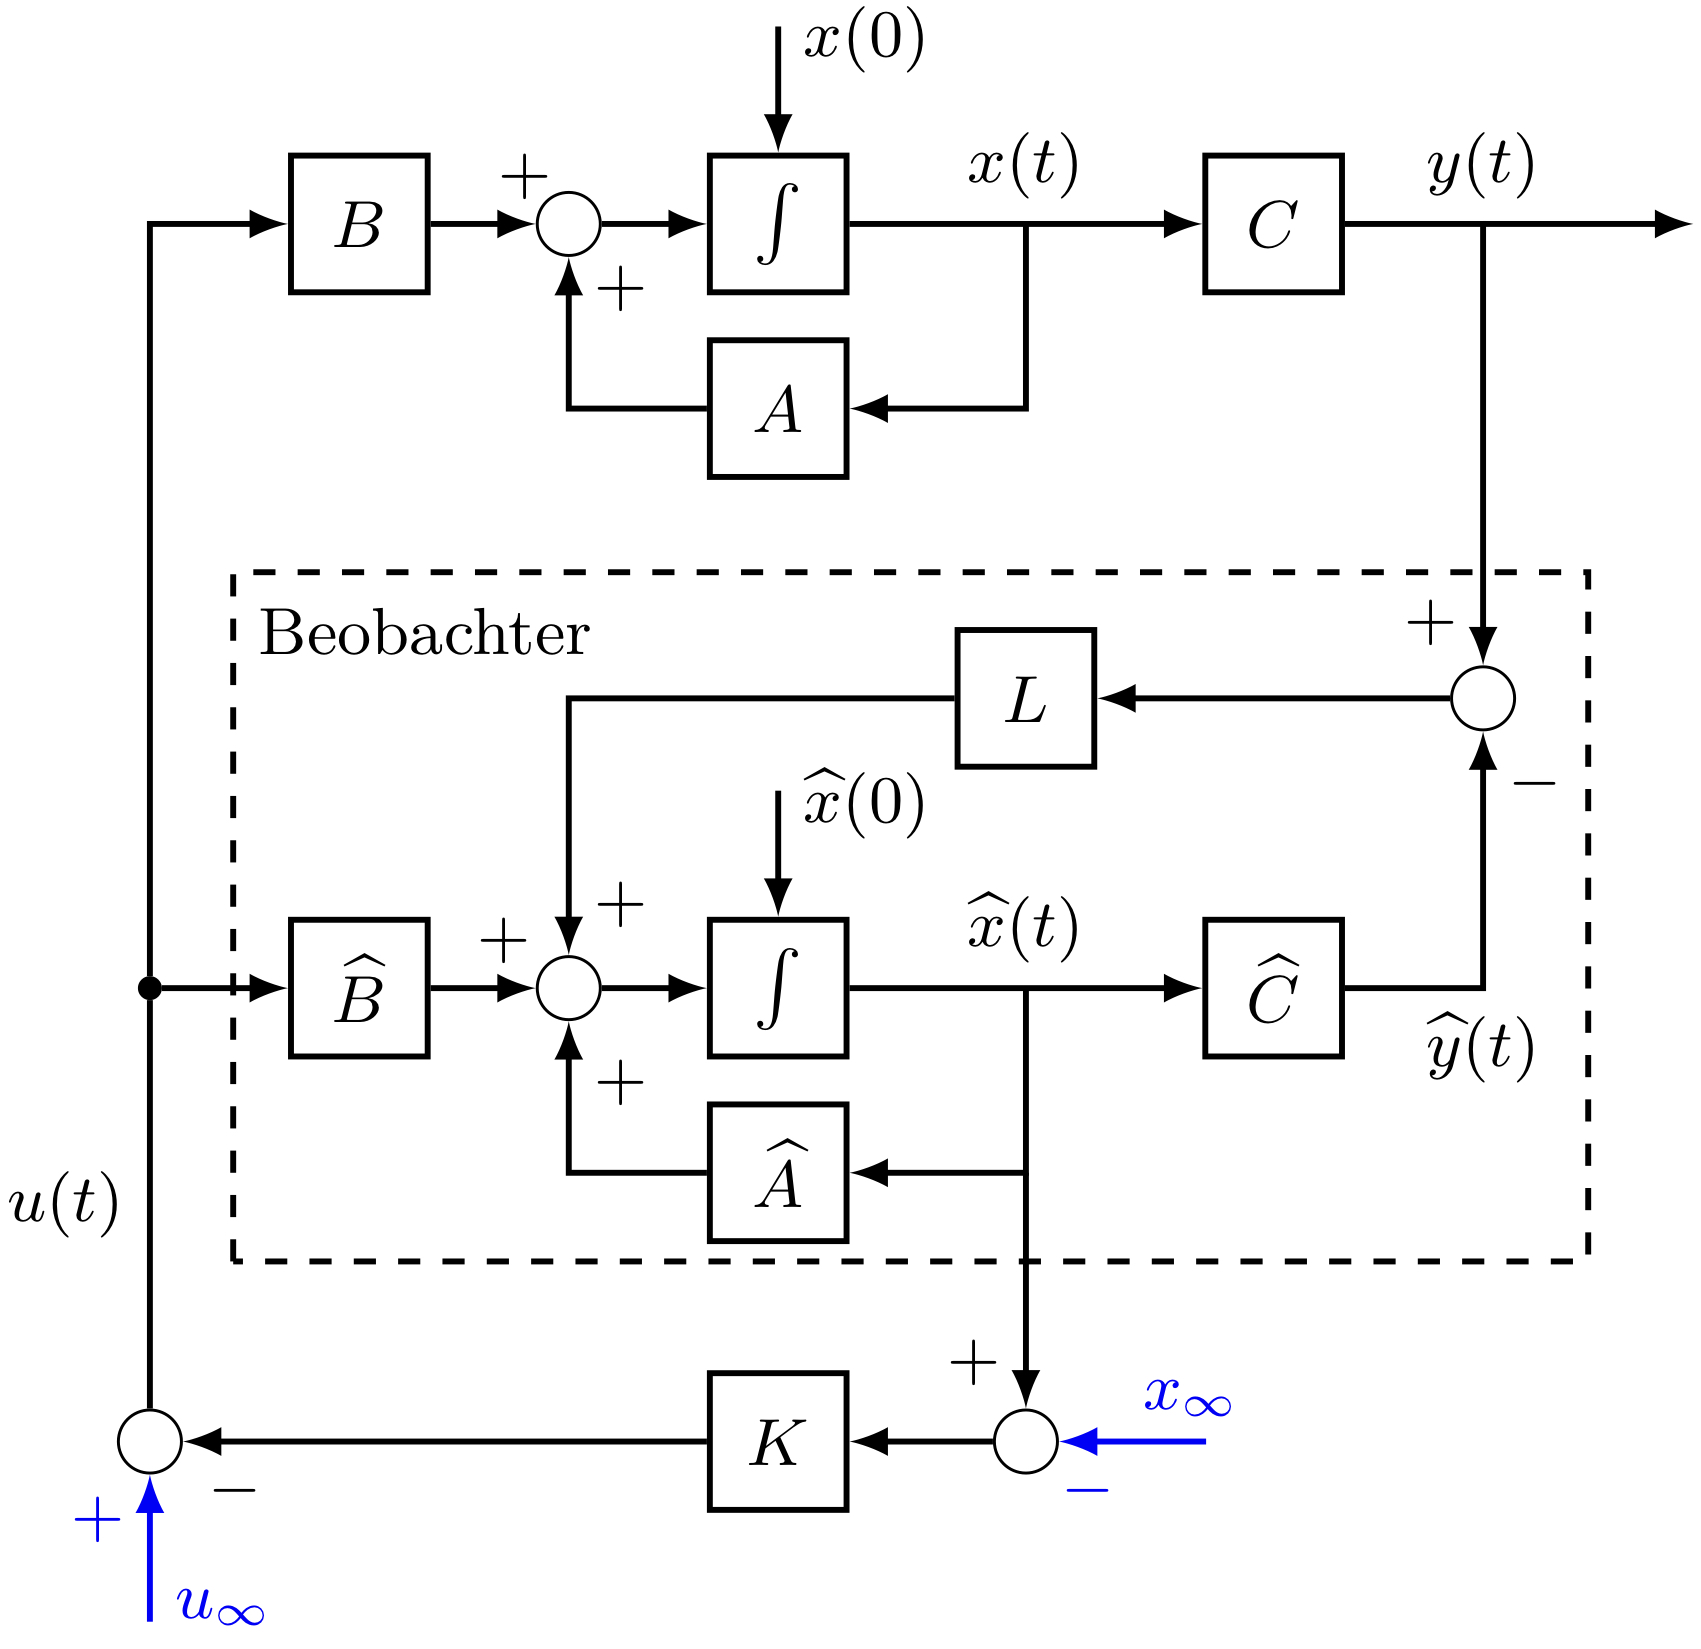
\includegraphics[width = 0.6\linewidth]{images/10/LQG_Folg.jpeg}
        \caption{LQG mit Folgeregelung durch $\{x_\infty,\, u_\infty\}$}
        \label{fig:lqgfolgeregelung}
    \end{figure}
    
    \subsubsection{Folgeregelung durch Vorsteuerung} \label{s:LQGIFolgeregelung}
        Die Struktur aus Abb. \ref{fig:lqgfolgeregelung} kann auch durch eine Folgeregelung auf die Referenz $r(t)$ umsetzen. 
        
        \begin{equation*}
            r(t) = \begin{bmatrix}r_1\\r_2\\\hdots\\r_m\end{bmatrix},\quad
            r(t) = \underbrace{y_\infty}_{= \textnormal{Const.}} = C\cdot x_\infty
        \end{equation*}
        \begin{figure}[H]
            \centering
            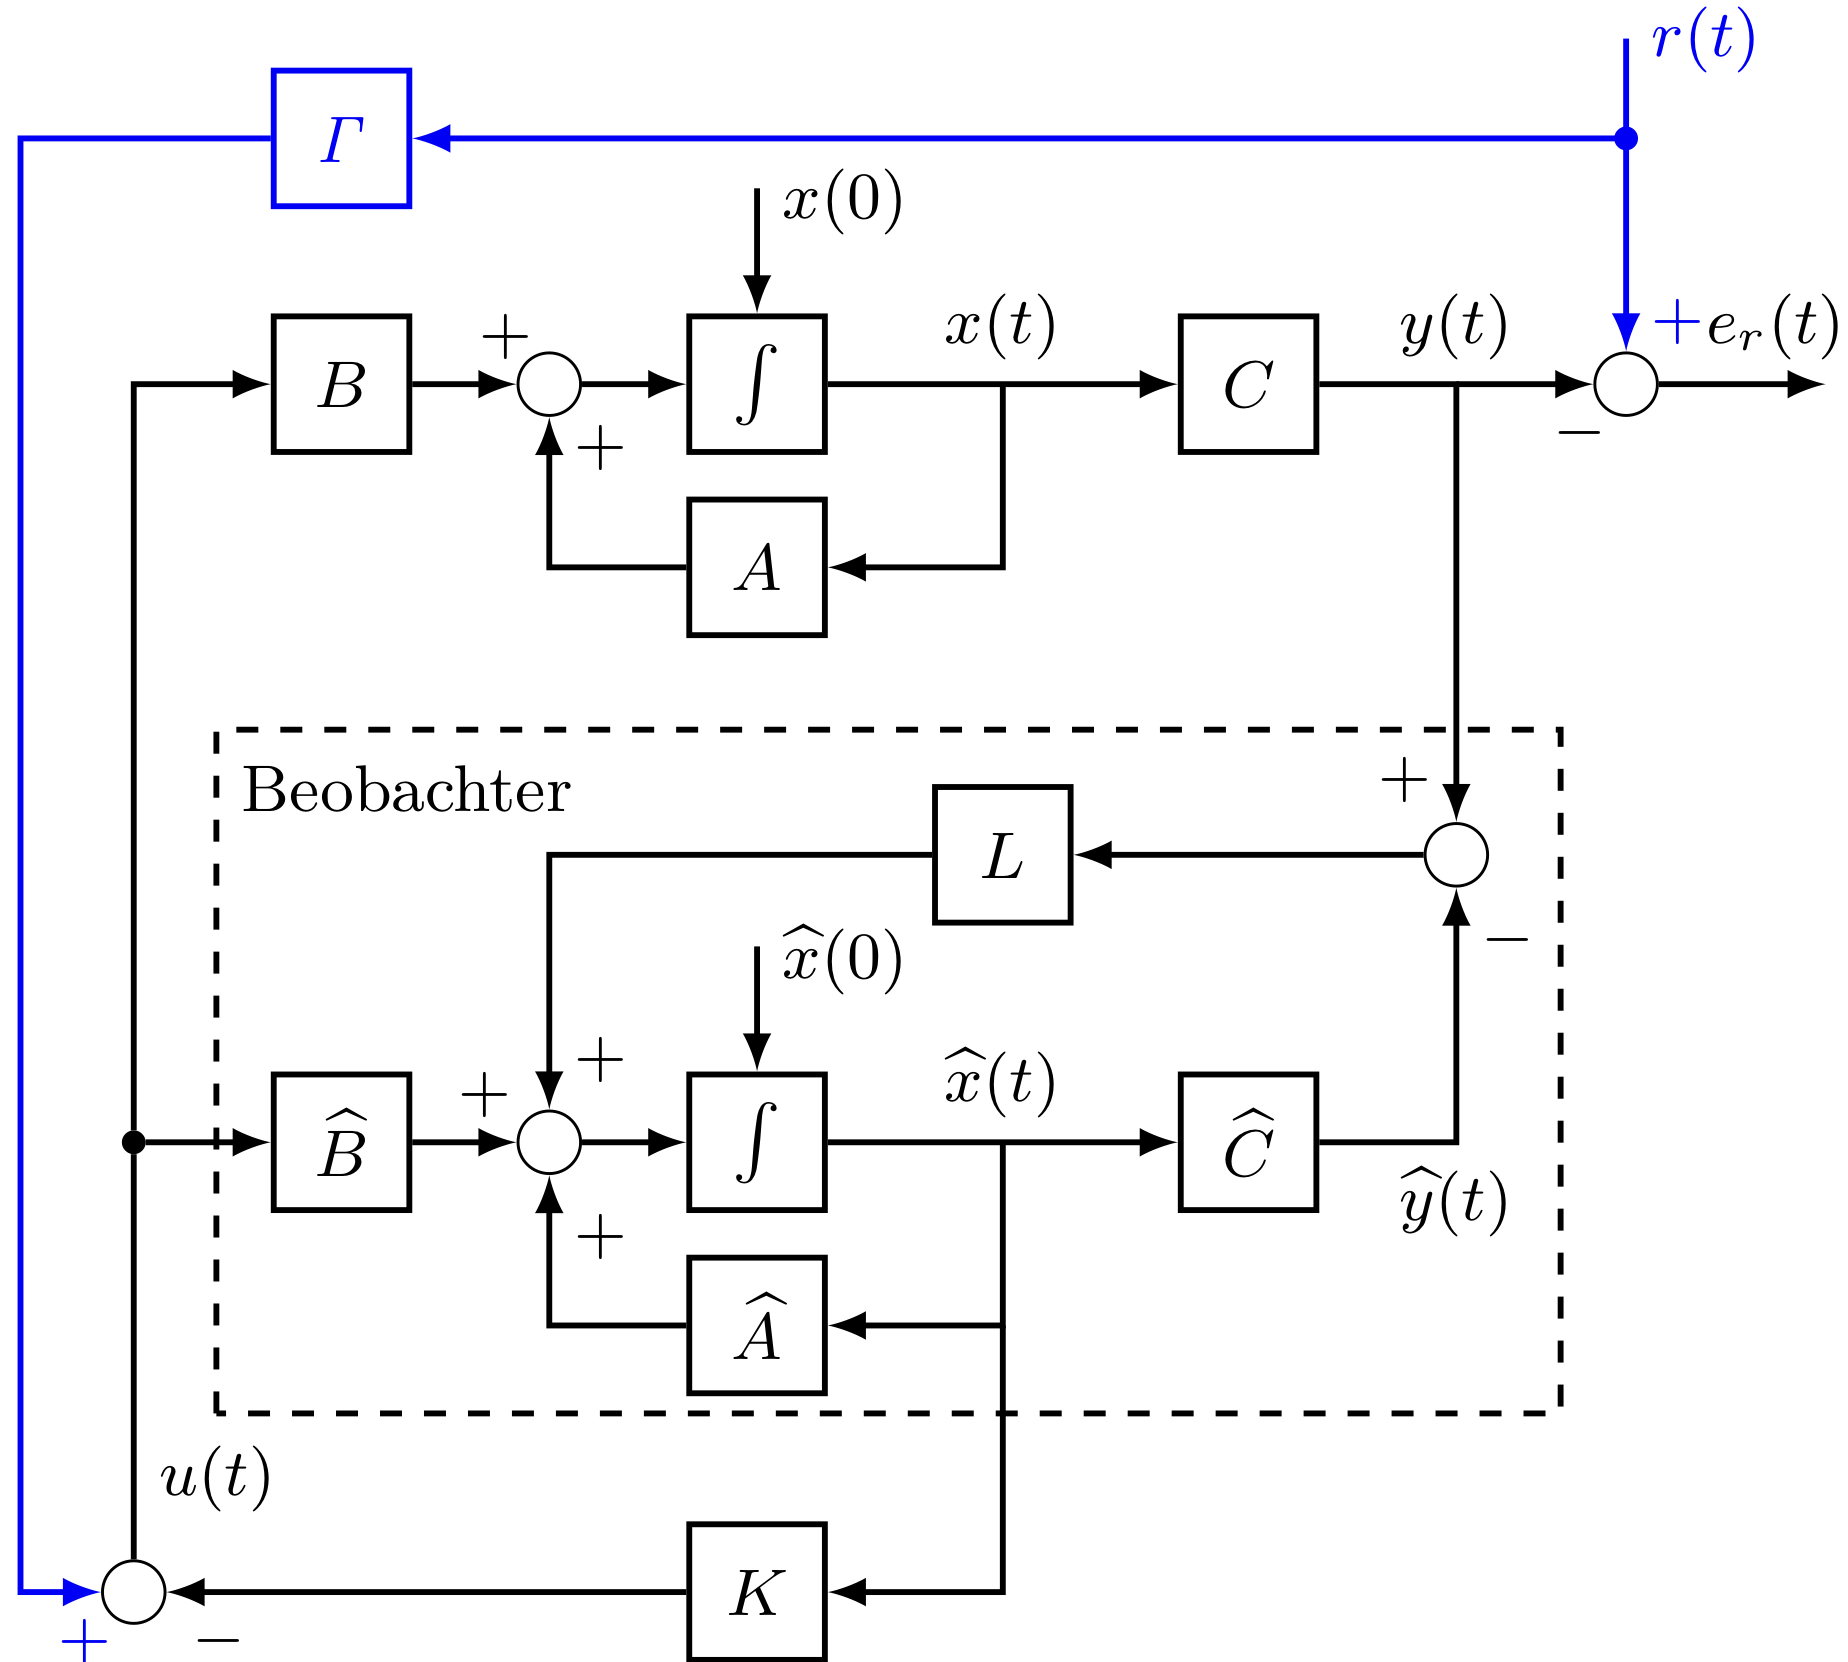
\includegraphics[width = 0.6\linewidth]{images/10/LQG_Folg_Vorst.jpeg}
            \caption{LQG Folgeregelung durh Vorsteuerung}
        \end{figure}
        Daraus ergeben sich folgende steady-state Gleichungen
        \begin{align*}
            0 &= A\cdot x_\infty + B\cdot u_\infty\\
            r(t) &= C\cdot x_\infty\\
            \Rightarrow \begin{bmatrix}0\\r(t)\end{bmatrix} &= 
            \underbrace{\begin{bmatrix}
            A & B\\
            C & 0
            \end{bmatrix}}_{F} \cdot
            \begin{bmatrix}x_\infty\\u_\infty\end{bmatrix}
        \end{align*}
        Falls $F$ vollen rang hat, kann man für $r(t)\rightarrow\{x_\infty,\, u_\infty\}$ folgende Beziehung herleiten.
        \begin{align*}
            u_\infty + K\cdot x_\infty &= \underbrace{-\Big(C\cdot\big(A-B\cdot K\big)^{-1}\cdot B\Big)^{-1}}_{\mathit{\Gamma}} \cdot r(t)\\
            &= \mathit{\Gamma}\cdot r(t)
        \end{align*}
    \subsection{LQGI zur Disturbance Rejection}
    Eine unbekannte Störung $w(t)$ wirkt additiv auf den Eingang $u(t)$ von $P(t)$ (kann auch an anderen Stellen angreifen. Ist für LQGI egal) aber nicht auf den Beobachter.
    
    Wir führen einen neuen Zustand für das System ein:
    \begin{align*}
        v(t) &= \int_0^t \big(0-y(\tau)\big)d\tau\\
        \Tilde{x}(t) &= \begin{bmatrix}x(t)\\\widehat{x}(t)\\v(t)\end{bmatrix},\quad \Tilde{x}(t)\in\mathbb{R}^{2n+m}
    \end{align*}
    Das Eingangssignal erweitert sich zu
    \begin{equation*}
        -K\cdot\widehat{x}(t) + K_I\cdot v(t),
    \end{equation*}
    wobei die Varibalen $K,\, K_I$ aus der LQRI-Formulierung stammen:
    \begin{gather*}
        \{\Tilde{A},\Tilde{B},\Tilde{Q},R\}\rightarrow \Tilde{K}= [K,-K_I]\\
        \Tilde{A}=\begin{bmatrix}A & 0\\ -C & 0\end{bmatrix},\quad \Tilde{B} = \begin{bmatrix}B\\0\end{bmatrix},\quad \Tilde{Q} = \begin{bmatrix} Q & 0\\ 0 & \gamma\cdot I\end{bmatrix}
    \end{gather*}
    Je Tiefer $\gamma$, desto langsamer das Integratorverhalten.
    
    \begin{figure}[H]
        \centering
        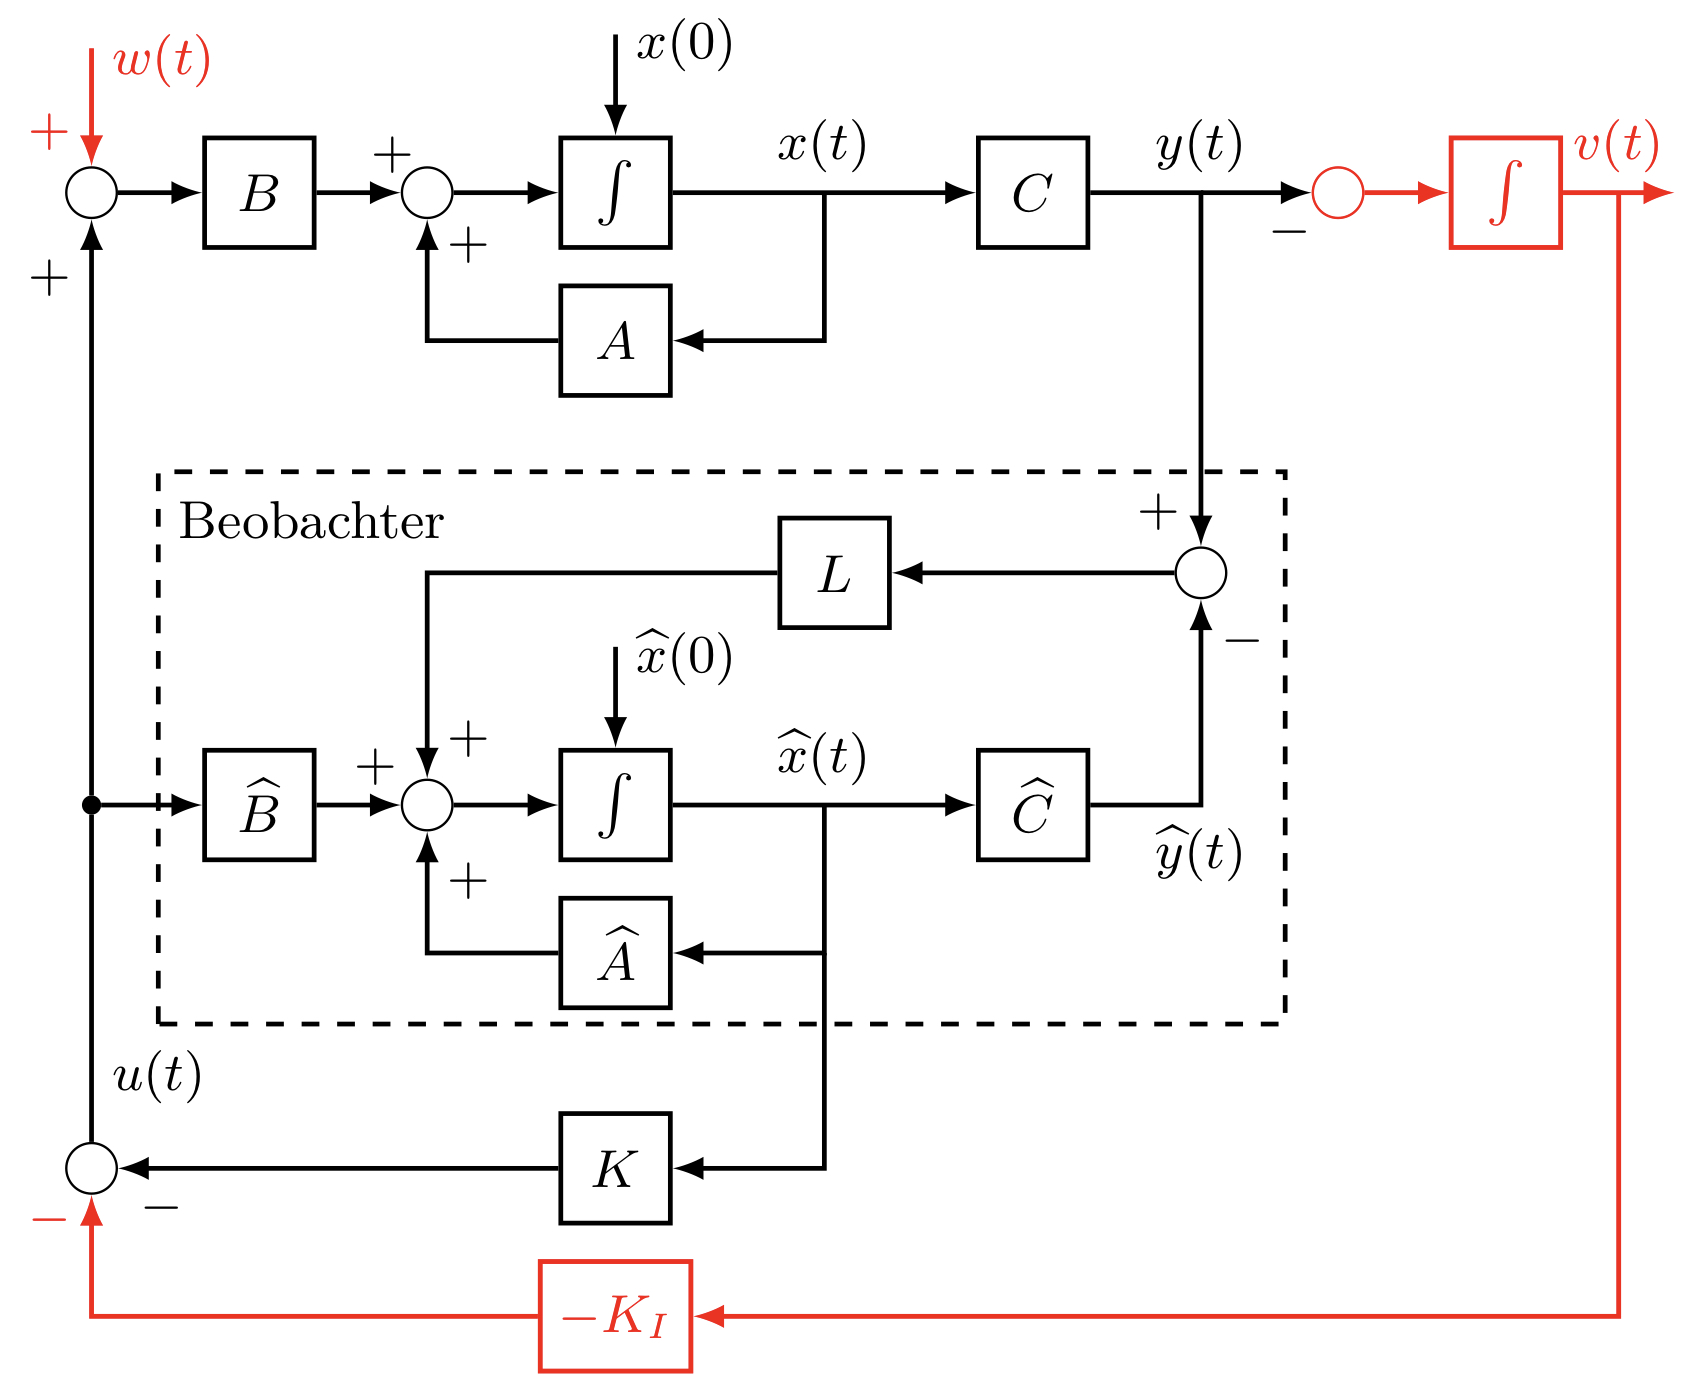
\includegraphics[width = 0.7\linewidth]{images/10/LQGI_distrejec.jpeg}
        \caption{Blockdiagramm für LQGI mit Störungsunterdrückung}
    \end{figure}
    
    \begin{figure}[H]
        \centering
        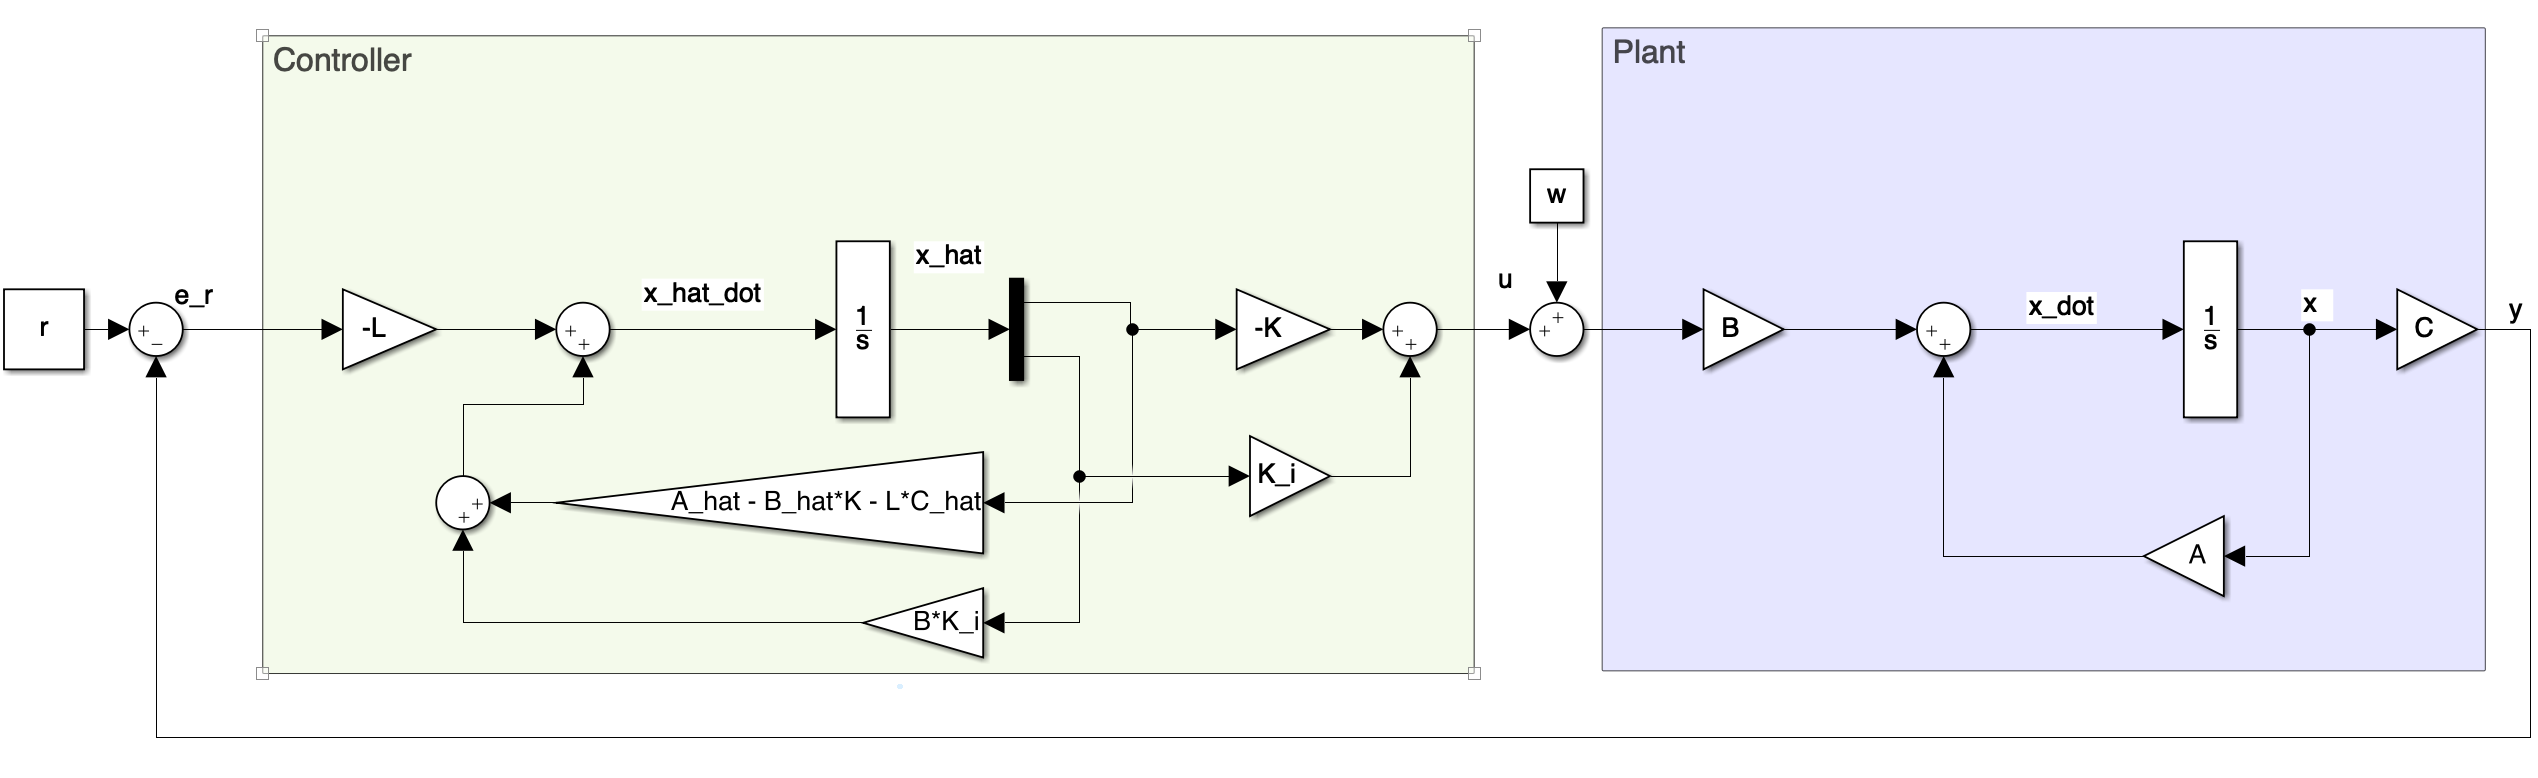
\includegraphics[width = \linewidth]{images/10/LQGI_alt.png}
        \caption{Alternative Dastellung des LQGI Reglers.}
        \label{fig:lqgialt}
    \end{figure}
    In dieser Darstellung von Abb. \ref{fig:lqgialt} enstpricht $\Tilde{x} = \begin{bmatrix}\widehat{x} \\ v\end{bmatrix}$ und $-L = \begin{bmatrix}-L\\ I \end{bmatrix}$. Die Dynamik des Observers ist dadurch gegeben als:
    \begin{align*}
        \Dot{\Tilde{x}}(t) &= \begin{bmatrix} \widehat{A}-\widehat{B}K - L\widehat{C} & BK_I\\
        0 & 0
        \end{bmatrix}\Tilde{x} + \begin{bmatrix} -L \\ I \end{bmatrix} e \quad (e = r-y = -y)\\
        u &= \begin{bmatrix} -K & K_I \end{bmatrix}\Tilde{x}
    \end{align*}
        
\subsection{LQGI mit Folgeregelung}
    LQGI mit Folgeregelung folgt aus der Kombination der beiden Ansätze. Dabei änder sich der Zustand $v(t)$ zu
    \begin{equation*}
        v(t) = \int_0^t \big(r(\tau)-y(\tau)\big)d\tau.
    \end{equation*}
    Das Eingangssignal resultiert als:
    \begin{equation*}
        u(t) = \mathit{\Gamma}\cdot r(t) - K \cdot\widehat{x}(t)+K_I\cdot v(t),
    \end{equation*}
    wobei $ \mathit{\Gamma}$ Gleich definiert ist wie in Abschnitt \ref{s:LQGIFolgeregelung}.
    
    \begin{figure}[H]
        \centering
        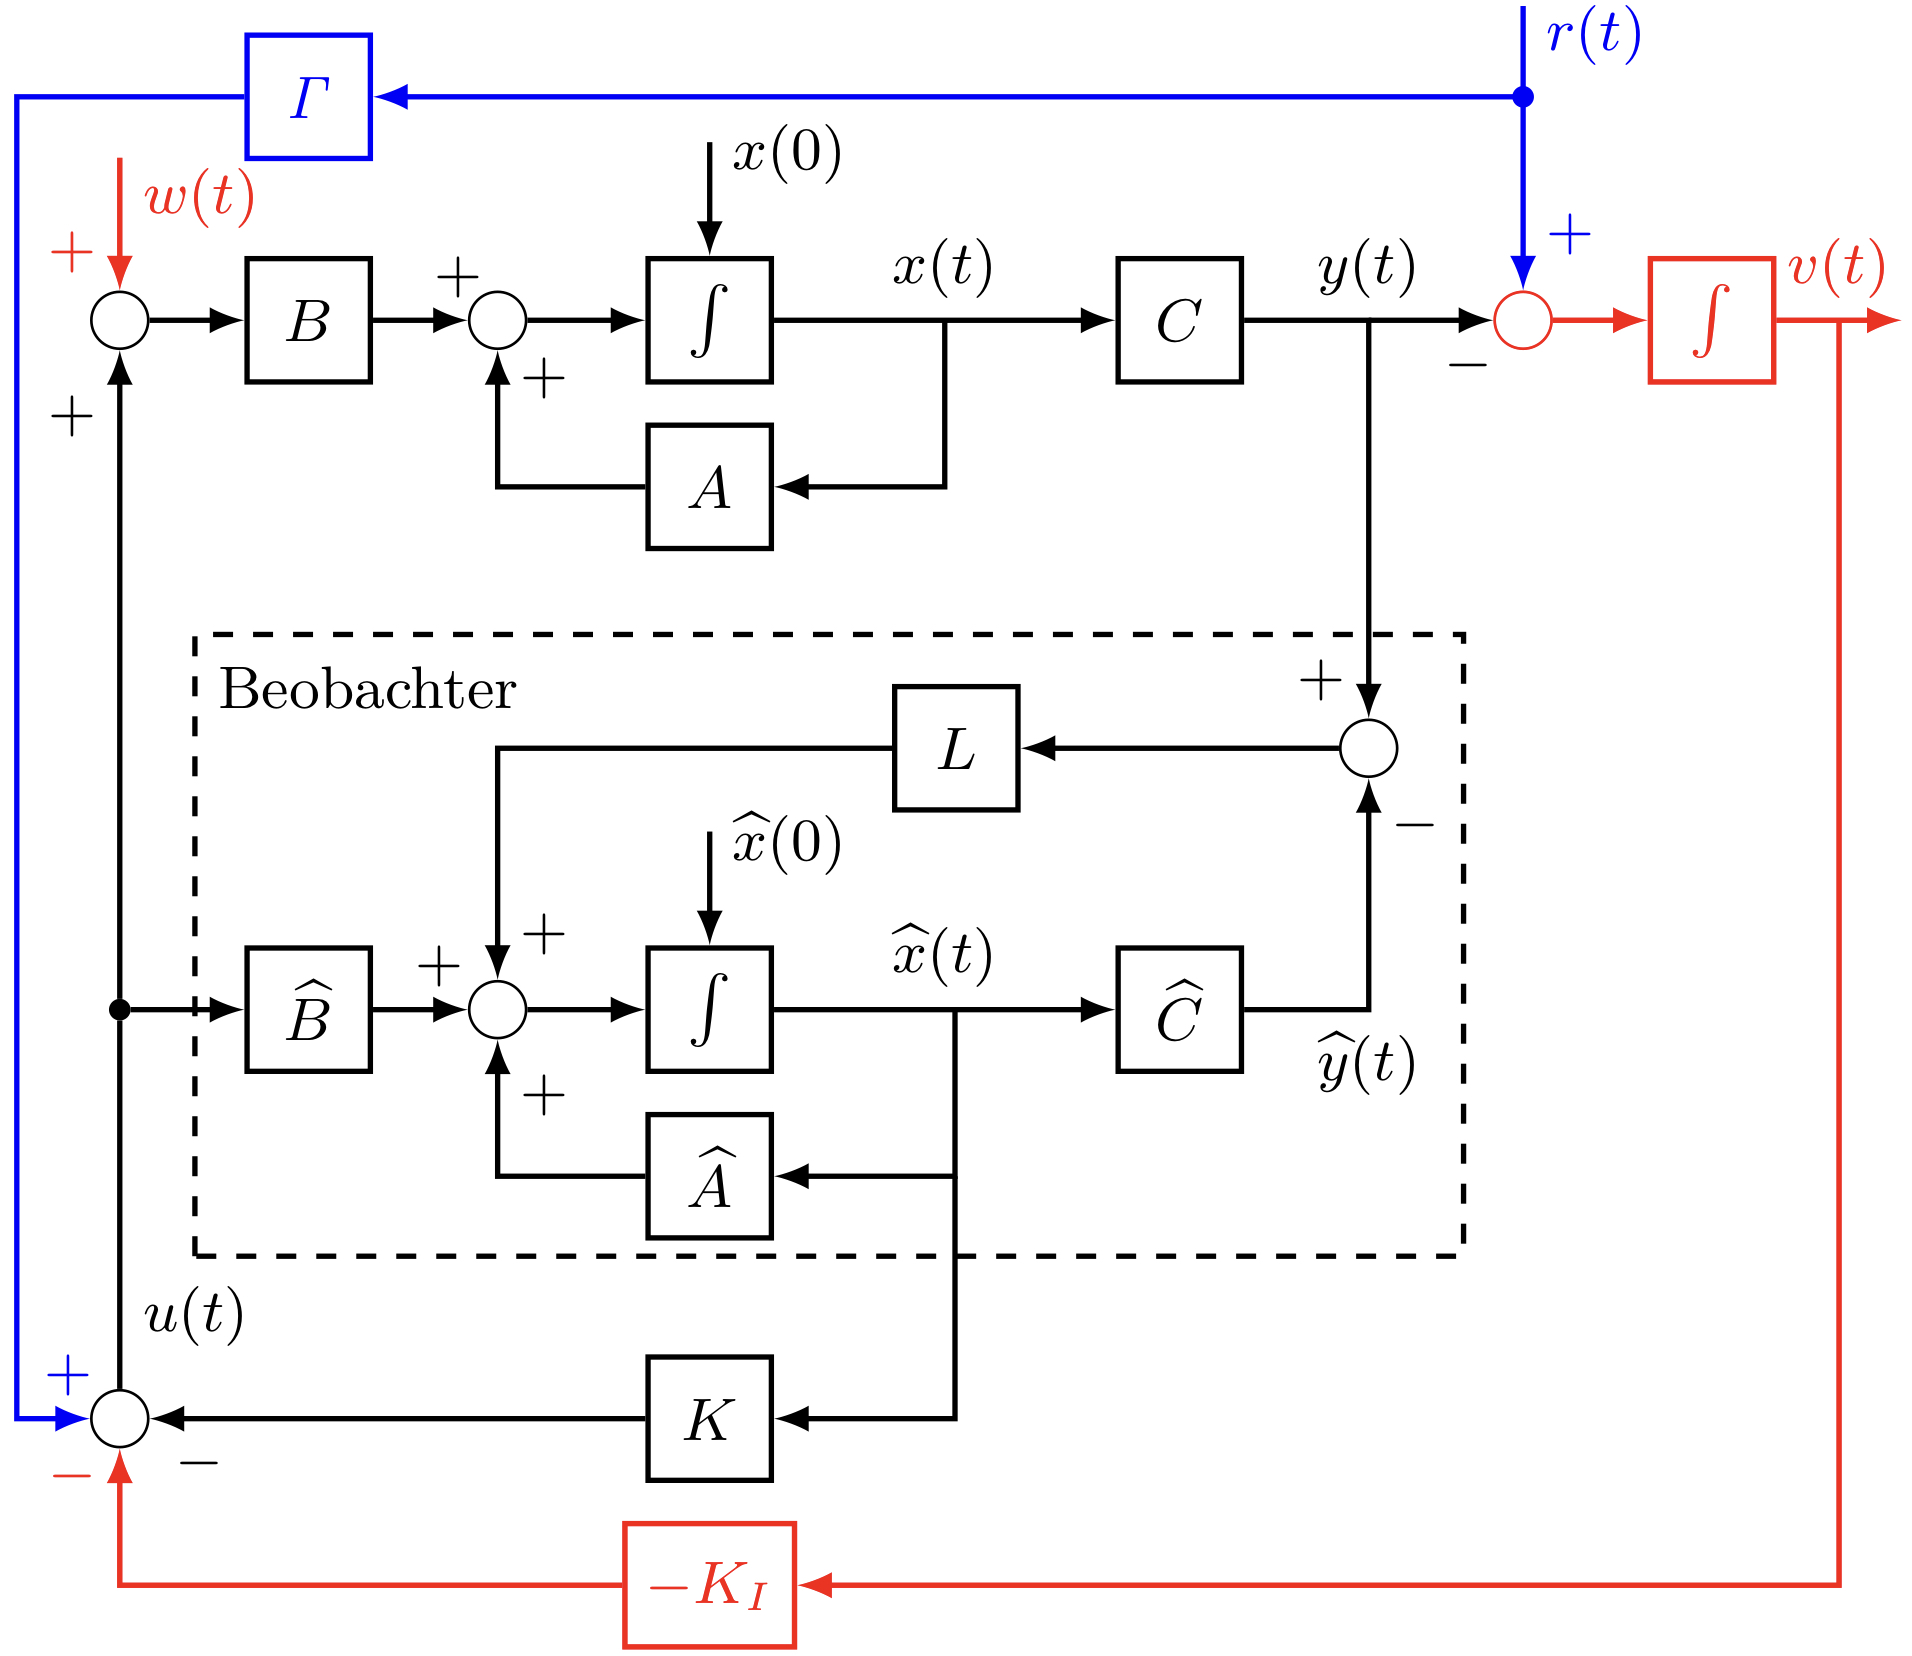
\includegraphics[width = 0.7\linewidth]{images/10/LQGI_Vorstr.jpeg}
        \caption{LQGI mit Vorsteuerung}
    \end{figure}
    
    \subsubsection{Auslegungsvorgehen}
        Die Auslegung eines LQGI-Reglers mit Folgeregelung verläuft nach diesem Rezept:
        
        \begin{enumerate}
            \item LQRI-Regler designen: $\{\Tilde{A},\Tilde{B},\Tilde{Q},\Tilde{R}\}\rightarrow \Tilde{K} = [K, -K_I]$, dabei werden $\Tilde{Q},\, R$ iterativ eingestellt
            
            \item Obersever designen: $\{A^\top, C^\top,\Bar{B}\cdot\Bar{B}^\top,q\cdot I\}\rightarrow L^\top$, dabei werden $\Bar{B},\, q$ iterativ eingestellt.
            
            \item Hinzufügen der Vorsteuerung für die Folgeregelung über die Matrix $\mathit{\Gamma}$.
        \end{enumerate}
    \subsection{Resultierende Regelkreise}
    Für alle betrachteten Regelkreise ist es möglich die resultierenden Systemgleichungen der offenen und geschlossenen Regelkreise darzustellen, wobei $e_r = r-y$:
    \begin{align*}
        \textnormal{Offener Regelkreis}\, L(s) &: e_r \rightarrow y\\
        \textnormal{Geschlossener Regelkreis}\, T(s) &: r \rightarrow y\\
    \end{align*}
    Betrachtung offener Regelkreis $\rightarrow$ Robustheitsbetrachtungen,
    
    Geschlossener Regelkreis $\rightarrow$ Stabilitätsverhalten, transientes Verhalten.
    
    \begin{align*}
        \frac{d}{dt}x(t) &= A\cdot x(t) + B\cdot u(t)\\
        \frac{d}{dt}\widehat{x}(t) &= A\cdot \widehat{x}(t) + B\cdot u(t) + L\big(y(t)-\widehat{y}(t)\big)\\
        \frac{d}{dt}v(t) &= r(t) - y(t),\quad\textnormal{(nur bei integrativen Strukturen)}\\
        y(t) &= C\cdot x(t),\,\textnormal{mit}\\
        \Tilde{x}(t) &=\begin{bmatrix}x(t)\\\widehat{x}(t)\end{bmatrix}\,\textnormal{oder}\, \Tilde{x}(t) =\begin{bmatrix}x(t)\\\widehat{x}(t)\\v(t)\end{bmatrix}
    \end{align*}
    
    \subsubsection{LQG-Regler}
        Regelgesetz:
        \begin{equation*}
            u(t) = -K\cdot\widehat{x}(t),\quad\textnormal{mit}\, r(t) = 0\,\textnormal{und}\, e_r = 0-y(t)
        \end{equation*}
        Offener Regelkreis:
        \begin{equation*}
            \frac{d}{dt}\Tilde{x}(t) = 
            \begin{bmatrix}
            A   & -BK\\
            0   &   A-BK-LC
            \end{bmatrix}\cdot\Tilde{x}(t) +
            \begin{bmatrix} 0\\ -L\end{bmatrix}\cdot e_r(t)
        \end{equation*}
        Geschlossener Regelkreis:
        \begin{equation*}
            \frac{d}{dt}\Tilde{x}(t) = 
            \begin{bmatrix}
            A   & -BK\\
            LC   &   A-BK-LC
            \end{bmatrix}\cdot\Tilde{x}(t) +
            \begin{bmatrix} 0\\ -L\end{bmatrix}\cdot r(t)
        \end{equation*}
        
     \subsubsection{LQG-Regler mit Folgeregelung}
        Regelgesetz:
        \begin{equation*}
            u(t) = \mathit{\Gamma}-K\cdot\widehat{x}(t)
        \end{equation*}
        Offener Regelkreis:
        \begin{equation*}
            \frac{d}{dt}\Tilde{x}(t) = 
            \begin{bmatrix}
            A +B\mathit{\Gamma}C   & -BK\\
            LC +B\mathit{\Gamma}C  &   A-BK-LC
            \end{bmatrix}\cdot\Tilde{x}(t) +
            \begin{bmatrix} B\\ B\end{bmatrix}\cdot \mathit{\Gamma}\cdot e_r(t)
        \end{equation*}
        Geschlossener Regelkreis:
        \begin{equation*}
            \frac{d}{dt}\Tilde{x}(t) = 
            \begin{bmatrix}
            A   & -BK\\
            LC &   A-BK-LC
            \end{bmatrix}\cdot\Tilde{x}(t) +
            \begin{bmatrix} B\\ B\end{bmatrix}\cdot \mathit{\Gamma}\cdot r(t)
        \end{equation*}
        
    \subsubsection{LQGI-Regler zur Störungsunterdrückung}
        Regelgesetz:
        \begin{equation*}
            u(t) = -K\cdot\widehat{x}(t) + K_I\cdot v(t),\quad\textnormal{mit}\, r(t) = 0
        \end{equation*}
        Offener Regelkreis:
        \begin{equation*}
            \frac{d}{dt}\Tilde{x}(t) = 
            \begin{bmatrix}
            A   & -BK &   BK_I\\
            0   &   A-BK-LC &   BK_I\\
            0   &   0   &   0
            \end{bmatrix}\cdot\Tilde{x}(t) +
            \begin{bmatrix} 0\\ -L\\ I\end{bmatrix}\cdot e_r(t)
        \end{equation*}
        Geschlossener Regelkreis:
        \begin{equation*}
            \frac{d}{dt}\Tilde{x}(t) = 
            \begin{bmatrix}
            A   & -BK &   BK_I\\
            LC   &   A-BK-LC &   BK_I\\
            -C  &   0   &   0
            \end{bmatrix}\cdot\Tilde{x}(t) +
            \begin{bmatrix} 0 & B\\ -L & 0\\ I & 0\end{bmatrix}\cdot \begin{bmatrix}r(t)\\w(t)\end{bmatrix}
        \end{equation*}
        
    \subsubsection{LQGI-Regler mit Folgeregelung}
        Regelgesetz:
        \begin{equation*}
            u(t) = \mathit{\Gamma} - K\cdot\widehat{x}(t) + K_I\cdot v(t),\quad\textnormal{mit}\, r(t) = 0
        \end{equation*}
        Offener Regelkreis:
        \begin{equation*}
            \frac{d}{dt}\Tilde{x}(t) = 
            \begin{bmatrix}
            A + B\mathit{\Gamma}C & -BK &   BK_I\\
            LC + B\mathit{\Gamma}C   &   A-BK-LC &   BK_I\\
            0   &   0   &   0
            \end{bmatrix}\cdot\Tilde{x}(t) +
            \begin{bmatrix} B\mathit{\Gamma}\\ B\mathit{\Gamma}\\ I\end{bmatrix}\cdot e_r(t)
        \end{equation*}
        Geschlossener Regelkreis:
        \begin{equation*}
            \frac{d}{dt}\Tilde{x}(t) = 
            \begin{bmatrix}
            A   & -BK &   BK_I\\
            LC   &   A-BK-LC &   BK_I\\
            -C  &   0   &   0
            \end{bmatrix}\cdot\Tilde{x}(t) +
            \begin{bmatrix} B\mathit{\Gamma} & B\\ B\mathit{\Gamma} & 0\\ I & 0\end{bmatrix}\cdot \begin{bmatrix}r(t)\\w(t)\end{bmatrix}
        \end{equation*}
        
\subsection{Berechnung der Übertragungsfunktionen}
    Die offenen Regelkreise haben die Struktur
    \begin{equation*}
    \colorboxed{red}{
    \begin{aligned}
        \frac{d}{dt}\tilde{x}(t) &= \Tilde{A}_\textnormal{ol}\cdot\tilde{x}(t) + \tilde{B}_\textnormal{ol}\cdot e_r(t)\\
        y(t) &= \underbrace{\big[C\ 0\big]}_{\tilde{C}_\textnormal{ol}}\cdot \tilde{x}(t)
    \end{aligned}
    }
    \end{equation*}
    Für die gescchlossenen Regelkreise folgen die Systemmatrizen $\{\tilde{A}_\textnormal{cl},\, \tilde{B}_\textnormal{cl},\, \tilde{C}_\textnormal{cl}\}$ anolg.
    
    Die Übertragungsfunktion der offenen Regelkreise $L(s)$ von $e_r\rightarrow y$ lautet somit:
    \begin{equation*}
    \colorboxed{red}{
        L_{\textnormal{LQG}}(s) = \tilde{C}_\textnormal{ol}\cdot\big(s\cdot I - \tilde{A}_\textnormal{ol}\big)^{-1}\cdot \tilde{B}_\textnormal{ol}
    }
    \end{equation*}
    
    Identisch kann man mit $(\cdot)_{\textnormal{cl}}$ die komplementäre Sensitivität $T(s)$ von $r\rightarrow y$ berechnen:
    \begin{equation*}
    \colorboxed{red}{
        T_{\textnormal{LQG}}(s) = \tilde{C}_\textnormal{cl}\cdot\big(s\cdot I - \tilde{A}_\textnormal{cl}\big)^{-1}\cdot \tilde{B}_\textnormal{cl}
    }
    \end{equation*}
    
    \subsubsection{Bsp}
        Der open-loop gain für den Standart LQG-Regler ergibt sich also aus
        \begin{align*}
            L_{\textnormal{LQG}}(s) &= 
            \underbrace{\begin{bmatrix}
            C & 0
            \end{bmatrix}}_{\tilde{C}_\textnormal{ol}}\cdot
            \underbrace{\begin{bmatrix}
            s\cdot I - A    &   BK\\
            0               &   s\cdot I - (A - BK - LC)
            \end{bmatrix}^{-1}}_{(sI-\tilde{A}_\textnormal{ol})^{-1}}\cdot
            \underbrace{\begin{bmatrix}
            0\\-L
            \end{bmatrix}}_{\tilde{B}_\textnormal{ol}}\\
            &=\underbrace{C\cdot(s\cdot I - A)^{-1}\cdot B}_{\textnormal{Plant}} \cdot \underbrace{K\cdot\big(s\cdot I - (A - BK - LC)\big)^{-1}\cdot L}_{\textnormal{Controller}}
        \end{align*}
        Aufgrund der Struktur von $\tilde{C}_\textnormal{ol}$ und $\tilde{B}_\textnormal{ol}$ muss in diesem Fall nur der Eintrag oben rechts der Inversen berechnet werden.
    
% \vfill\null\columnbreak
\section{Wiederherstellung der Robustheit}
    \subsection{Minimum Return difference LQR/LQG}
Der offene LQR-Regelkreis 
\begin{equation*}
    L_{\textnormal{LQR}} = K\cdot \big(s\cdot I - A\big)^{-1}
\end{equation*}
besitzt hervorragende Robustheitseigenschaften:
\begin{equation*}
    \mu_{\textnormal{min,\textbf{LQR}}} = \min_\omega\bigg( \min_i\sigma_i\Big(I + L_{\textnormal{\textbf{LQR}}}(\jw)\Big)\bigg) \geq 1
\end{equation*}
Jedoch kann keine Aussage zur minimum return difference des LQG-Reglers gemacht werden.
\begin{equation*}
    \mu_{\textnormal{min,\textbf{LQG}}} = \min_\omega\bigg( \min_i\sigma_i\Big(I + L_{\textnormal{\textbf{LQG}}}(\jw)\Big)\bigg) \geq \ ?
\end{equation*}
Man muss nach der Reglerauslegung deshalb zwingend die Robustheit des Reglers überprüfen.

\subsection{Loop-Transfer Recovery LTR}
    Man kann die Robustheit des ursprünglichen LQR-Reglers mit einem LQG Regler approximieren. Dafür muss der Observer sehr schnell gewählt werden. Dadurch konvergiert der Fehler $e(t) = x(t)- \widehat{x}(t)$ schnell zu Null (im Grenzfall unendlich schnell). Diese Wiederherstellung der Robustheit nennt man \textit{loop-transfer recovery (LTR)}.
    
    \textbf{Erinnerung:} Je kleiner man den tuning-Parameter $q$ wählt, desto schneller wird die Dynamik des Fehlers (Schneller $\widehat{=} \ \operatorname{eig}\big(A - L(q)\cdot C\big)$ sind weiter links in der kommplexen Ebene)
    
    \subsubsection{Dynamik des Fehlers in der Zustandsschätzung}
        Analyse des Fehlers für $\displaystyle\lim_{q\to0}(\cdot)$.
        \begin{equation*}
            \lim_{q\to0}e(t) = \lim_{q\to0}\big(A - L(q)\cdot C\big)^{-1}\cdot\Dot{e}(t) = 0
        \end{equation*}
        Da $\big(A - L(q)\cdot C\big)$ Hurwitz ist und $\operatorname{eig}(X^{-1}) = 1/\operatorname{eig}(X)$ gilt,  konvergieren die Eigenwerte von $\big(A - L(q)\cdot C\big)$ asymptotisch gegen null. Mit $e(t) = x(t) - \widehat{x}(t)$ folgt:
        \begin{equation*}
            \lim_{q\to0} \widehat{x}(t) = x(t), \quad \forall t
        \end{equation*}
        
        Das System verhält sich für kleine $q$ als ob keine Beobachterdynamik vorhanden wäre. Für $q\to 0$ Verhält sich ein LQG-Regler wie ein LQR-Regler und besitzt somit die gleichen Robustheitseigenschaften.
        
        \textbf{Bemerkungen:}
        \begin{itemize}
            \item $q$ kann in der Realität nicht beliebig klein gewählt werden, da ansonst hochfrequentes Rauschen massiv Verstärkt wird.
            
            \item Falls die Regelstrecke nicht-miniphasige NST hat, approximiert der LTR-Ansatz den LQR-Regler häufig so gut wie möglich. (Bei nicht-miniphasigen Systemen. ist die durchtrittsfrequenz nah oben beschränkt und dadurch ist eine perfekte Approximation der LQR-Regelung nicht möglich.)
        \end{itemize}
        
        \begin{figure}[H]
            \centering
            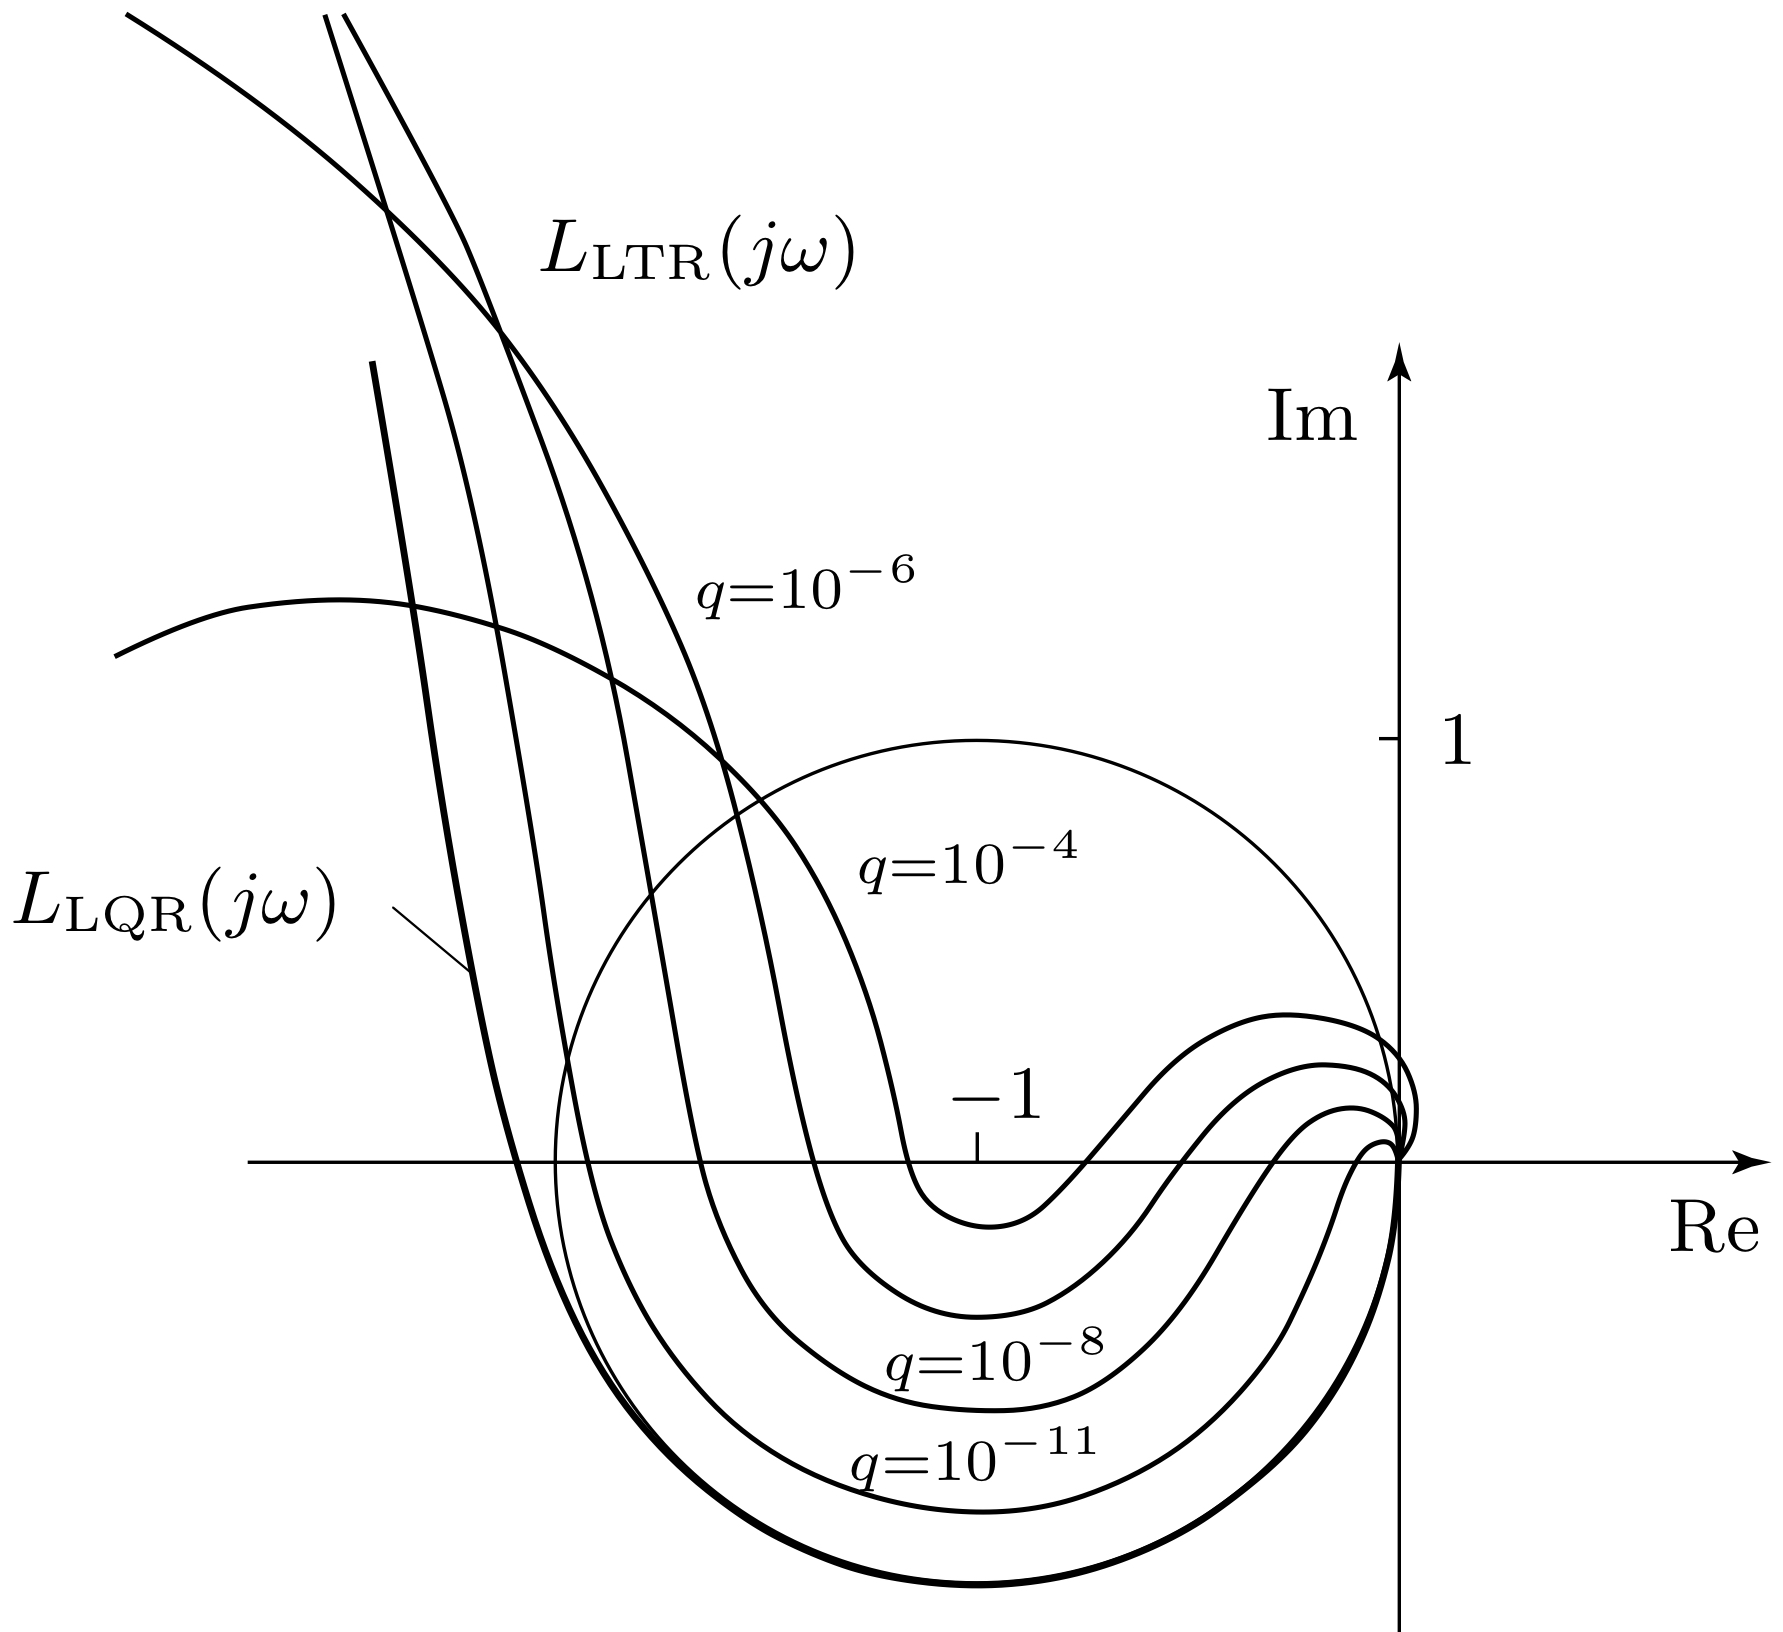
\includegraphics[width = 0.6\linewidth]{images/11/L_LTR.jpeg}
            \caption{$L_{\textnormal{LTR}}$ für verschiedene $q$.}
        \end{figure}
        
    
\end{multicols*}     

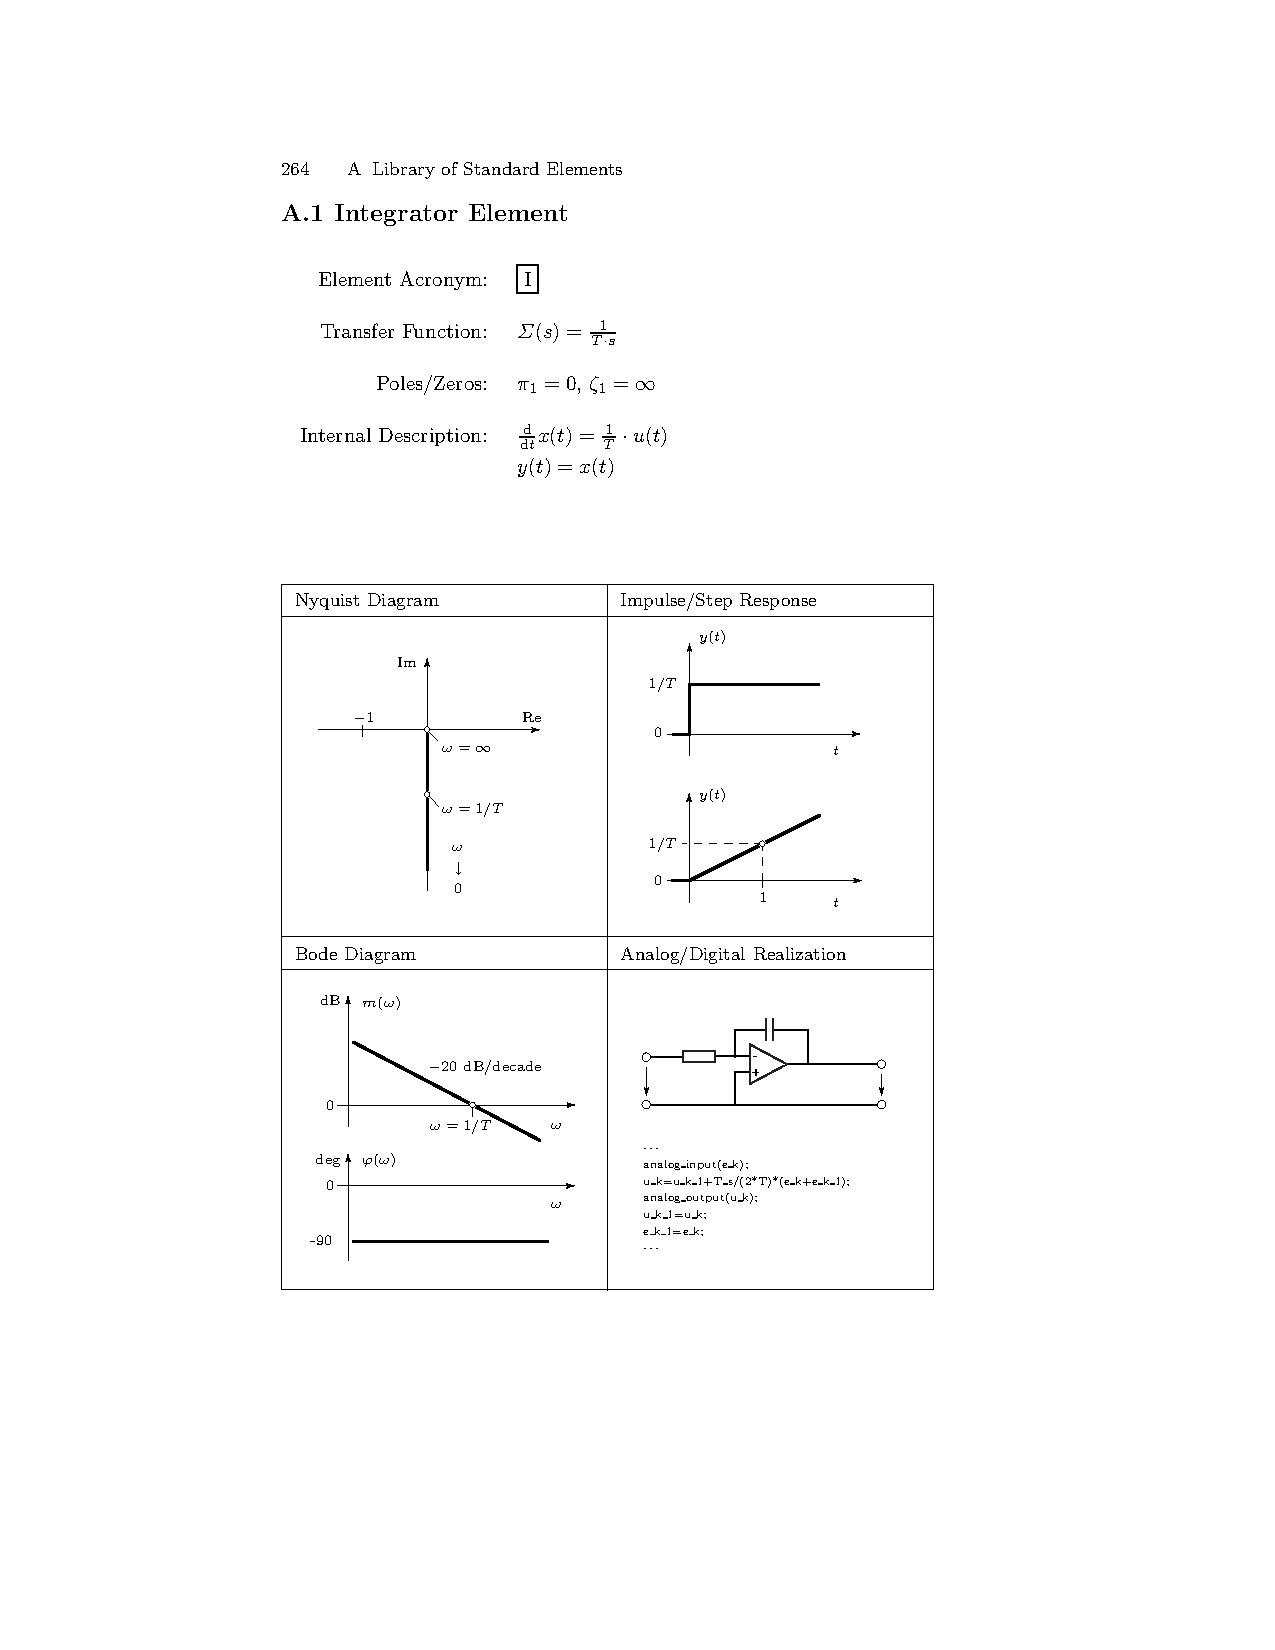
\includepdf[pages=-, nup=2x1, delta= -10mm -10mm, addtotoc={1, section, 1, {Appendix A}, appendix}]{resources/Guzzella_RT1_Appendix_A.pdf}

\end{document}